\chapter{Cubed-sphere finite-volume methods}
\label{chp-cs-fv}
Now that we have described in Chapter \ref{chp-cs-grids} how we can obtain the ghost cell values of each panel on the cubed-sphere using Lagrange interpolation, we are ready to apply the dimension-splitting methods presented in Chapter \ref{chp-2d-fv} to solve the advection equation on the cubed-sphere.
One significant difference is that we have the metric term, which is not present in the plane simulations.
Additionally, when employing ghost cell layers using the duo-grid, the flux at the cube edges is computed twice, 
requiring the averaging of fluxes at the edges to ensure a unique value in order to achieve mass conservation.


This Chapter is organized as follows: Section \ref{chp-cs-adv} introduces the advection equation on the cubed-sphere.
Section \ref{chp-cs-fvcs} presents its finite-volume discretization with a focus on the extension of dimension splitting (Section \ref{sec-csdsplit}) 
as presented in Section \ref{sec-dsplit}.
Numerical experiments are presented in Section \ref{chp-cs-numexpadv}, where we use dimension splitting to assess its
accuracy in computing the divergence of a given vector field to check its numerical consistency, as well as to solve the advection equation.
In particular, we explore different treatments for the cube edges. Section \ref{chp-cs-conc} presents the final thoughts.

\section{Cubed-sphere advection equation in integral form}
\label{chp-cs-adv}
Given a tangent velocity field $\boldsymbol{u}$ on the sphere, we denote its
contravariant components by $\mathfrak{u}$ and $\mathfrak{v}$.
We shall use all the notations introduced in Section \ref{cs-notation}.
The advection equation on panel the $p$ of the cubed-sphere with initial condition $q_0$ is given by:
\begin{equation}
	\begin{cases}
		\label{eq1-adv-cs}
		\bigg[{\partial}_t{q}+
		\frac{1}{\sqrt{\mathfrak{g}}}\bigg(
		{\partial}_x{(\mathfrak{u} q \sqrt{\mathfrak{g}})}+
		{\partial}_y{(\mathfrak{v} q \sqrt{\mathfrak{g}})}
		\bigg)\bigg](x,y,p,t)
		= 0,\\
		q(x,y,p,0) = q_0(x,y,p),
	\end{cases}
\end{equation}
$\forall (x,y) \in \Omega := [-\alpha,\alpha]^2$, $t\in[0,T]$.
We denote by $\nabla \cdot (q\boldsymbol{u})$ the divergence operator:
\begin{equation}
	\label{advcs:eqdiv}
	\nabla \cdot (q\boldsymbol{u})(x, y, p, t) =  \frac{1}{\sqrt{\mathfrak{g}}}
	[{\partial_x (\mathfrak{u}q\sqrt{\mathfrak{g}})} + {\partial_y (\mathfrak{v}q\sqrt{\mathfrak{g}})}](x, y, p, t).
\end{equation}
We recall that we say the $\boldsymbol{u}$ is \textbf{non-divergent} if $\nabla \cdot \boldsymbol{u}=0$.
We define the $\mathcal{CS}_N$ grid function $\delta^n$ as
the exact divergence of $q\boldsymbol{u}$ at the cell centers, namely
\begin{equation}
	\label{cs-discrete-div}
	\delta^n_{ijp} = \nabla \cdot (\boldsymbol{u}q)(x_i,y_j,p,t^n).
\end{equation}
In this Chapter, it shall be useful to define the average value of $q\sqrt{\mathfrak{g}}$ on the 2D coordinates as:
\begin{equation}
\label{cs-q-av}
\overline{(\sqrt{\mathfrak{g}}q)}_{ijp}(t) = \frac{1}{\Delta x \Delta y}
\int_{x_{i-\frac{1}{2}}}^{x_{i+\frac{1}{2}}}
\int_{y_{j-\frac{1}{2}}}^{y_{j+\frac{1}{2}}}  q(x,y,p,t) {\sqrt{\mathfrak{g}}(x,y)}\,dx \,dy.
\end{equation}
This average value simplifies the deduction of finite-volume method on the cubed-sphere instead of using the spherical average values (Equation \eqref{qav-sphere}).
Since the metric term does not depend on $t$, we may rewrite Equation \eqref{eq1-adv-cs} as
\begin{equation}
	\label{eq2-adv-cs}
	\bigg[{\partial}_t{(q \sqrt{\mathfrak{g}})}+
	{\partial}_x{(\mathfrak{u}q \sqrt{\mathfrak{g}})}+
	{\partial}_y{(\mathfrak{v}q \sqrt{\mathfrak{g}})}
	\bigg](x,y,p,t)
	= 0.
\end{equation}
Therefore, as in Problem \eqref{chp-adv2d-sec2-prob1}, the integral form of Equation \eqref{eq1-adv-cs}
is stated in Problem \eqref{chp5-prob1}.
\begin{prob}
	\label{chp5-prob1}
	Given an initial condition ${q}_0$ and
	a velocity on the sphere $\boldsymbol{u}$, with contravariant components $(\mathfrak{u},\mathfrak{v})$ on the cubed-sphere coordinate system,
	we would like to find a weak solution ${q}$
	of the cubed-sphere advection equation in its integral form:
	\begin{align*}
		\int_{x_1}^{x_2} \int_{y_1}^{y_2}
		{(q\sqrt{\mathfrak{g}})}(x, y, p, t) \,dx \,dy = &\int_{x_1}^{x_2} \int_{y_1}^{y_2}
		{(q\sqrt{\mathfrak{g}})}(x, y, p, t) \,dx \,dy \\ \nonumber
		&-\int_{t_1}^{t_2} \int_{y_1}^{y_2} \bigg({(\mathfrak{u}q\sqrt{\mathfrak{g}})}(x_2, y, t)
		-{(\mathfrak{u}q\sqrt{\mathfrak{g}})}(x_1, y, t) \bigg) \,dy \,dt\\ \nonumber
		&-\int_{t_1}^{t_2} \int_{x_1}^{x_2} \bigg({(\mathfrak{v}q\sqrt{\mathfrak{g}})}(x, y_2, t)
		-{(\mathfrak{v}q\sqrt{\mathfrak{g}})}(x, y_1, t) \bigg) \,dx \,dt.
	\end{align*}
	$\forall [x_1, x_2]\times [y_1, y_2] \times[t_1, t_2] \subset \Omega \times[0,T]$, and
	$q(x,y,p,0)=q_0(x,y,p)$.
\end{prob}
Similarly to Section \ref{chp-adv2d-sec1}, Equation \eqref{eq1-adv-cs} and Problem \eqref{chp5-prob1} are equivalent
when ${q}, \boldsymbol{u} \in \mathcal{C}^1(\mathbb{S}^2_R)$.
For Problem \ref{chp5-prob1}, the total mass in $\mathbb{S}^2_R$ is defined by: 
\begin{equation}
	{M}_{\mathbb{S}^2_R}(t) = \sum_{p=1}^6 \int_{\Omega} {(q\sqrt{\mathfrak{g}})}(x,y,p,t) \,dx \,dy , \quad \forall t \in [0,T],
\end{equation}
and is conserved within time: 
\begin{equation}
	{M}_{\mathbb{S}^2_R}(t) = {M}_{\mathbb{S}^2_R}(0), \quad \forall t \in [0,T].
\end{equation}
We define a discretized version of Problem \eqref{chp5-prob1} as Problem \eqref{chp5-prob2}.
\begin{prob}
	\label{chp5-prob2}
	Assume the framework of Problem \ref{chp5-prob1}
	and consider a $(\Delta x, \Delta y, \Delta t, \lambda)$-discretization of $\Omega\times [0,T]$, with $\Delta x= \Delta y$.
	Since we are in the framework of Problem \ref{chp5-prob1}, it follows that:
	\begin{align*}
		\overline{(\sqrt{\mathfrak{g}}q)}_{ijp}(t_{n+1})  = \overline{(\sqrt{\mathfrak{g}}q)}_{ijp}(t_{n})
		&- { \lambda}
		\delta _x \bigg( \frac{1}{\Delta t \Delta y}
		\int_{t^n}^{t^{n+1}} \int_{y_{j-\frac{1}{2}}}^{y_{j+\frac{1}{2}}} 
		{(\mathfrak{u}q\sqrt{\mathfrak{g}})}(x_{i}, y, p, t)
		\,dy \,dt \bigg) \\ \nonumber
		&- {\lambda}
		\delta _y \bigg( \frac{1}{\Delta t \Delta x}
		\int_{t^n}^{t^{n+1}} \int_{x_{i-\frac{1}{2}}}^{x_{i+\frac{1}{2}}} 
		{(\mathfrak{v}q\sqrt{\mathfrak{g}})}(x, y_{j}, p, t)
		\,dx \,dt \bigg),
	\end{align*}
	where
	\begin{equation}
		\overline{(\sqrt{\mathfrak{g}}q)}_{ijp}(t) = \frac{1}{\Delta x \Delta y}
		\int_{x_{i-\frac{1}{2}}}^{x_{i+\frac{1}{2}}} 
		\int_{y_{j-\frac{1}{2}}}^{y_{j+\frac{1}{2}}} {(q\sqrt{\mathfrak{g}})}(x,y,p,t) \,dx \,dy.
	\end{equation}
	Our problem now consists of finding the values ${Q}_{ijp}(t_{n})$, 
	$\forall i = 1, \ldots, N$, $\forall j = 1, \ldots, M$, $\forall n = 0, \ldots, N_T-1$,
	given the initial values ${(\sqrt{\mathfrak{g}}q)}_{ijp}(0)$, $\forall i = 1, \ldots N$, $\forall j = 1, \ldots, M$.
	In other words, we aim to find the average values of ${(\sqrt{\mathfrak{g}}q)}_{ijp}$ in each control volume $\Omega_{ijp}$ at the specified time instances.
\end{prob}
It is important to note that no approximations have been made in Problems \eqref{chp5-prob1} and \eqref{chp5-prob2}. 
%In practice, the term $\frac{\Delta x  \Delta y}{|\Omega_{ijp}|}$ is estimated using the second-order
%formula obtained by applying the midpoint rule in Equation \eqref{chp4-area}:
%\begin{equation}
%	\frac{\Delta x  \Delta y}{|\Omega_{ijp}|}= \frac{1}{\sqrt{\mathfrak{g}}_{ijp}} + O(\Delta x^2).
%\end{equation}
\section{Finite-volume on the cubed-sphere approach}
\label{chp-cs-fvcs}
We are ready to introduce the finite-volume scheme on the cubed-sphere (CS-FV).
A CS-FV scheme problem as follows in Problem \ref{chp5-prob3}.
Before that, we consider the following approximation, which follows from the midpoint rule (Theorem \ref{prop-bound-midpoint2d}):
\begin{equation}
	\label{midpoint-approx}
	\overline{(\sqrt{\mathfrak{g}}q)}_{ijp}(t)  = \sqrt{\mathfrak{g}_{ij}} {q}_{ijp}(t) +\mathcal{O}(\Delta x^2).
\end{equation}
We use this approximation in Problem{chp5-prob2} and we obtain the following CS-FV scheme:
\begin{prob}[CS-FV scheme]
	\label{chp5-prob3}
	Assume the framework defined in Problem \ref{chp5-prob2}.
	The finite-volume approach of Problem \ref{chp5-prob1}
	consists of a finding a scheme of the form:
	\begin{align}
		\label{chp5-csfv}
		{q}_{ijp}^{n+1} =  {q}_{ijp}^{n} - \frac{\lambda}{\sqrt{\mathfrak{g}}_{ij}} \delta_i {F}_{ijp}^{n}
		-  \frac{\lambda}{\sqrt{\mathfrak{g}}_{ij}}  \delta_j {G}_{ijp}^{n},
		\\ \nonumber \quad \forall i = 1, \ldots, N, \quad \forall j = 1, \ldots, M, \quad p =1, \ldots, 6,
		\quad \forall n = 0, \ldots, N_T-1,
	\end{align}
	where $ \delta_i F_{ijp}^n =
	{F}_{i+\frac{1}{2},j,p}^{n} 
	- {F}_{i-\frac{1}{2},j,p}^{n}$,
	$ \delta_j G_{ijp}^n =
	{G}_{i,j+\frac{1}{2},p}^{n} 
	- {G}_{i,j-\frac{1}{2},p}^{n}$ 
	and ${q}^{n}\in \mathcal{CS}_N$ is intended to be an approximation
	of ${q}(t_{n})\in \mathcal{CS}_N$ in some sense. We define
	${q}_{ijp}^{0} = {q}^0_{ijp}$.
	
	The term ${F}_{i+\frac{1}{2}, j, p}^{n}$ is known as numerical flux in the 
	$x$ direction and it approximates
	$\frac{1}{\Delta t \Delta y }\int_{t_n}^{t_{n+1}} 
	\int_{y_{j-\frac{1}{2}}}^{y_{j+\frac{1}{2}}} 
	(\mathfrak{u}q\sqrt{\mathfrak{g}})(x_{i+\frac{1}{2}}, y, p, t) \,dy \,dt $,
	$\forall i = 0, 1, \ldots, N$, and 
	${G}_{i, j+\frac{1}{2}, p}^{n}$ is known as numerical flux in the 
	$y$ direction and it approximates
	$\frac{1}{\Delta t\Delta x}\int_{t_n}^{t_{n+1}}  
	\int_{x_{i-\frac{1}{2}}}^{x_{i+\frac{1}{2}}}
	(\mathfrak{v}q\sqrt{\mathfrak{g}})(x, y_{j+\frac{1}{2}}, p, t) \,dx \,dt $,
	$\forall j = 0, 1, \ldots, M$,
	or, in other words, they estimate the time-averaged
	fluxes at the control volume $\Omega_{ijp}$ boundaries.
\end{prob}
\begin{remark}
	For Problem \ref{chp5-prob3}, we define the CFL number in the $x$ and $y$ direction
	by $\max \{{|\mathfrak{u}_{i+\frac{1}{2},j,p}^n}|\}\frac{\Delta t}{\Delta x}$ and 
	$\max \{ {|\mathfrak{v}_{i,j+\frac{1}{2},p}^n}|\}\frac{\Delta t}{\Delta y}$, respectively.
	The CFL number is maximum between these numbers and we say that the CFL condition is
	satisfied if the CFL number is less than one. 
\end{remark}
As we mentioned in Problem \ref{chp5-prob3}, the initial condition may be assumed as $q_{ijp}^0$ or $Q_{ijp}(0)$.
We are going to assume  $q_{ijp}^0$ as initial data to avoid the computation of integrals.
Furthermore, the errors will be calculated using the values $q_{ijp}^n$ instead of $Q_{ijp}(t_n)$.
As in Section \ref{sec:fv-2d} this approximation leads to a second-order error.


\section{Dimension splitting}
\label{sec-csdsplit}
In this Section, we will utilize the dimension splitting method described in Section \ref{sec-dsplit} to obtain a CS-FV scheme.
To facilitate notation, we shall omit the index $p$ whenever it may appear in this Section, as what is described here does not depend on $p$.
Also, the ghost cell values are assumed to be filled using the duo-grid interpolation.
\subsection{PPM and the metric term}
\label{sec-metricppm}
Recall that the dimension splitting technique requires the numerical solution of advection in the $x$ and $y$ directions for separability.
For instance, in the case of the advection equation on the cubed-sphere (Equation \eqref{eq2-adv-cs}), we need to solve the following equations in the $x$ direction:
\begin{equation}
	\label{1d-avd-eq}
		[{\partial_t (\sqrt{\mathfrak{g}} {q^x})} + {\partial_x (\mathfrak{u}\sqrt{\mathfrak{g}}{q^x}})](x, y_j, p, t),
\end{equation}
for $j=-\nu+1, \ldots, N+\nu$, at certain time levels $t^n$, $n=1, \ldots, N_T$ (Section \ref{lit-trotter-sp}).
We are particularly interested in approximating $q^{x,n+1}_{ij}$ for $i=1, \ldots, N$, which represents the values of $q^x$ at the cell centroids.
This involves providing an approximation of the solution to Equation \eqref{eq2-adv-cs}, 
denoted as $q^n_{ij}$, serving as initial data at time level $n$, specifically $q^{x,n}_{ij}=q^n_{ij}$.

Considering the midpoint approximation of the average value (Equation \eqref{midpoint-approx}), we approximate
the solution of the desired problem using an general 1D FV-SL scheme as discussed in Section \ref{chp-adv1d-sec2-fvsl}:
\begin{equation}
	\label{1d-qx}
	q^{x,n+1}_{ij} = q^{n}_{ij}  - \frac{\Delta t}{\sqrt{\mathfrak{g}_{ij}}\Delta x}
	\bigg[{F}_{i+\frac{1}{2},j}
	\big({q}^{n}; \tilde{c}^{x,n}\big) - 
	{F}_{i-\frac{1}{2},j}
	\big({q}^{n}; \tilde{c}^{x,n}\big)\bigg],
\end{equation}
for  $j=-\nu+1, \ldots, N+\nu$ and $i=1, \ldots, N$, where
\begin{equation}
	\label{mt0-flux}
	{F}_{i\pm\frac{1}{2},j} = \frac{1}{\Delta t}\int_{ \tilde{x}_{i\pm\frac{1}{2},j}^n}^{x_{i\pm\frac{1}{2}}}(\widetilde{\sqrt{\mathfrak{g}}{q}})_j(x, t^n) \,dx,
\end{equation}
$\tilde{x}_{i\pm\frac{1}{2},j}^n$ is an estimate of the departure point in $x$ direction using the time-averaged
CFL number $\tilde{c}^{x,n}_{i+\frac{1}{2},j}$ (Section \ref{chp-adv1d-sec-dp}),
and $\widetilde{\sqrt{\mathfrak{g}}{q}}_j$ is a PPM reconstruction (or any other reconstruction) of $\sqrt{\mathfrak{g}}{q}$ (Section \ref{chp-adv1d-sec-recon})
in the $x$ direction ($j$ is fixed).

It is also possible to compute the PPM reconstruction in terms only of $q$, ignoring the metric term $\sqrt{\mathfrak{g}}$.
In other words, we may assume that the metric is constant on each integration domain, which leads to the following first-order error:
\begin{equation}
\int_{ \tilde{x}_{i\pm\frac{1}{2},j}^n}^{x_{i\pm\frac{1}{2}}}(\widetilde{\sqrt{\mathfrak{g}}{q}})(x, t^n) \,dx
= \sqrt{\mathfrak{g}}_{i\pm\frac{1}{2},j}\int_{  \tilde{x}_{i\pm\frac{1}{2},j}^n}^{x_{i\pm\frac{1}{2}}}\widetilde{q}(x, t^n) \,dx + \mathcal{O}(\Delta x).
\end{equation}
In this case, the flux reads:
\begin{equation}
	\label{mt1-flux}
	{F}_{i\pm\frac{1}{2},j} =  \frac{\sqrt{\mathfrak{g}}_{i\pm\frac{1}{2},j}}{\Delta t}\int_{  \tilde{x}_{i\pm\frac{1}{2},j}^n}^{x_{i\pm\frac{1}{2}}}\widetilde{q}(x, t^n)  \,dx.
\end{equation}
Then, in this case, we perform the PPM flux for the grid function $q^n$.
When we compute the flux using Equation \eqref{mt0-flux}, we denote this by \textbf{mt0};
when using Equation \eqref{mt1-flux}, we denote this by \textbf{mt1}.

The works of \citet{lin:2004} and \citet{putman:2007} use the mt1 method, which is currently employed in FV3.
This process, although it introduces a first-order error, 
significantly simplifies the elimination of the splitting error that arises when $q_{ij} = \overline{q}$, for a constant $\overline{q}$, 
and when the wind is divergence-free.
This occurs because when we use mt1, we have
\begin{equation}
	\label{mt1-flux2}
	{F}_{i\pm\frac{1}{2},j} =  \overline{q}\frac{\sqrt{\mathfrak{g}}_{i\pm\frac{1}{2},j}}{\Delta t}
	\delta_i c^{x,n}_{ij},
\end{equation}
assuming that the departure point is computed using the DP1 method for the departure point calculation (as discussed in Section \ref{sp-error}).
The property from Equation \eqref{mt1-flux2} does not occur for mt0.

\subsection{The 2D scheme on each cube panel}
\label{sec-splittingcs}
For a CS-grid function $\psi \in \mathcal{CS}_N$
we introduce the following PPM flux in the $x$ direction (recall Equation \eqref{chp-sec-flux:numerical-flux8})
\begin{align}
	%	\label{chp3-flux-xdir}
	\mathfrak{F}_{i+\frac{1}{2},j}^{PPM,x} [{{\psi}^n;\tilde{c}^{x,n}}]= %\tilde{u}^{n}_{i+\frac{1}{2},j}\times
	\begin{cases}
		{\psi}_{i-1,j}^{n}+(1-\tilde{c}_{i+\frac{1}{2}}^{x,n})
		(b^L_{ij}-\tilde{c}_{i+\frac{1}{2},j}^{x,n})
		(b^L_{ij}+b^R_{ij}),
		\quad &\text{if} \quad \tilde{c}_{i+\frac{1}{2},j}^{x,n}>0,\\
		{\psi}_{ij}^{n}+(1+\tilde{c}_{i+\frac{1}{2},j}^{x,n})
		(b^L_{i+1,j}+\tilde{c}_{i+\frac{1}{2},j}^{x,n})
		(b^L_{i+1,j}+b^R_{i+1,j}),
		\quad &\text{if} \quad \tilde{c}_{i+\frac{1}{2},j}^{x,n}\leq0.
	\end{cases}
\end{align}
for each $j=-\nu+1, \ldots, N+\nu$ and $i=1, \ldots, N$, and
where the PPM perturbation values $b^L$ and $b^R$ values are computed using hord0 (Section \ref{chp-adv1d-sec-hord0}) or hord8 (Section \ref{chp-adv1d-sec-hord8})

Therefore, we may rewrite Equation \eqref{1d-qx} as
\begin{equation}
q^{x,n+1}_{ij} = q^{n}_{ij} + \mathbf{F}_{ij}[{q^n,\tilde{c}^{x,n}}],
\end{equation}
for $i=1, \ldots, N$, $j=-\nu+1, \ldots, M + \nu$, and where
\begin{align*}
	\mathbf{F}_{ij}[{q^n,\tilde{c}^{x,n}}] = 
	-\frac{1}{|\hat{\Omega}_{ij}|}
	\bigg(\mathcal{A}_{i+\frac{1}{2},j}^{x} \mathfrak{F}_{i+\frac{1}{2},j}^{x}[q^n_{\times,j},\tilde{c}^{x,n}]-
	\mathcal{A}_{i-\frac{1}{2},j}^{x} \mathfrak{F}_{i-\frac{1}{2},j}^{x}[q^n_{\times,j},\tilde{c}^{x,n}] \bigg),
\end{align*}
recalling the term $|\hat{\Omega}_{ij}|$ from defined Equation \eqref{chp4-area},
and following the discussion on the metric term, we have the coefficients
\begin{align}
	\mathcal{A}_{i+\frac{1}{2},j}^x= 
	\begin{cases}
		\hat{\delta} x_{i+\frac{1}{2},j}  \hat{\delta} y_{i+\frac{1}{2},j} 
		\sin{\alpha_{i+\frac{1}{2},j}}
		{\tilde{c}}_{i+\frac{1}{2},j}^{x,n},
		\quad &\text{for mt0},\\
		{\Delta x}{\Delta y}{\tilde{c}}_{i+\frac{1}{2},j}^{x,n}
		\quad &\text{for mt1},
	\end{cases}
\end{align}
where we have made use of Equation \eqref{distcube2} and Equation \eqref{mt-sina}, 
and the PPM fluxes are
\begin{align}
	\mathfrak{F}_{i+\frac{1}{2},j}^x [{{q}^n;\tilde{c}^{x,n}}] = 
	\begin{cases}
		\mathfrak{F}_{i+\frac{1}{2},j}^{PPM,x}[{{\sqrt{\mathfrak{g}}q}^n;\tilde{c}^{x,n}}]
		\quad &\text{for mt0},\\
		\mathfrak{F}_{i+\frac{1}{2},j}^{PPM,x}[{{q}^n;\tilde{c}^{x,n}}]
		\quad &\text{for mt1}.
	\end{cases}
\end{align}
Similarly, we may derive a scheme to solve Equation \eqref{eq2-adv-cs} in the $y$ direction as
\begin{equation}
	q^{y,n+1}_{ij} = q^{n}_{ij} + \mathbf{G}_{ij}[{q^n,\tilde{c}^{x,n}}],
\end{equation}
for $i=-\nu+1, \ldots, N + \nu$  $j=1, \ldots, N$.
\begin{align*}
	\mathbf{G}_{ij}[{q^n,\tilde{c}^{y,n}}] = 
	-\frac{1}{|\hat{\Omega}_{ij}|}
	\bigg(\mathcal{A}_{i,j+\frac{1}{2}}^{y} \mathfrak{F}_{i,j+\frac{1}{2}}^{y}[q^n_{i,\times},\tilde{c}^{y,n}]-
	\mathcal{A}_{i,j-\frac{1}{2}}^{y} \mathfrak{F}_{i,j-\frac{1}{2}}^{y}[q^n_{i,\times},\tilde{c}^{y,n}] \bigg),
\end{align*}
and
\begin{align}
	\mathcal{A}_{i,j+\frac{1}{2}}^y= 
	\begin{cases}
		\hat{\delta} x_{i,j+\frac{1}{2}}  \hat{\delta} y_{i,j+\frac{1}{2}} 
		\sin{\alpha_{i,j+\frac{1}{2}}}
		{\tilde{c}}_{i,j+\frac{1}{2}}^{y,n},
		\quad &\text{for mt0},\\
		{\Delta x}{\Delta y}{\tilde{c}}_{i,j+\frac{1}{2}}^{y,n},
		\quad &\text{for mt1},
	\end{cases}
\end{align}
and the PPM fluxes are
\begin{align}
	\mathfrak{F}_{i,j+\frac{1}{2}} [{{q}^n;\tilde{c}^{y,n}}]= 
	\begin{cases}
		\mathfrak{F}_{i,j+\frac{1}{2}}^{PPM,y}[{{\sqrt{\mathfrak{g}}q}^n;\tilde{c}^{y,n}}]
		\quad &\text{for mt0},\\
		\mathfrak{F}_{i+\frac{1}{2},j}^{PPM,y}[{{q}^n;\tilde{c}^{y,n}}]
		\quad &\text{for mt1}.
	\end{cases}
\end{align}
In FV3, the terms ${\hat{\delta} x_{ij}}$ and ${\hat{\delta} y_{ij}}$ and $|\hat{\Omega}_{ij}|$ (for integers or half integers $i$ and $j$)
are replaced by ${{\delta} x_{ij}}$, ${{\delta} y_{ij}}$ and $|\hat{\Omega}_{ij}|$,
which represent the geodesic distances and areas (Section \ref{cs-geo}).
\begin{table}[!h]
	\begin{tabular}{|c|l|l|}
		\hline
		Scheme & \multicolumn{1}{c|}{$\mathbf{f}_{ij}(q^n, \tilde{c}^{x,n})$}
		& \multicolumn{1}{c|}{$\mathbf{g}_{ij}(q^n, \tilde{c}^{y,n})$} \\ \hline
		LT   & $\mathbf{F}_{ij}(q^n,\tilde{c}^{x,n})$ 
		& $\mathbf{G}_{ij}(q^n,\tilde{c}^{y,n})$ \\ \hline
		PL   & $-q_{ij}^n +
		\frac{q_{ij}^n  + \mathbf{F}_{ij}(q^n,\tilde{c}^{x,n})}
		{1 - \frac{1}{|\hat{\Omega}_{ij}|}\big(\mathcal{A}_{i+\frac{1}{2},j}^{x} - \mathcal{A}_{i-\frac{1}{2},j}^{x}\big)}$
		& $-q_{ij}^n +
		\frac{q_{ij}^n  + \mathbf{G}_{ij}(q^n,\tilde{c}^{y,n})}
		{1 - \frac{1}{|\hat{\Omega}_{ij}|}\ \big(\mathcal{A}_{i,j+\frac{1}{2}}^{y} - \mathcal{A}_{i,j-\frac{1}{2}}^{y}\big)}$
		\\ \hline
	\end{tabular}
	\caption{Expression of the inner advective operators considered in this work.
		LT stands for the average Lie-Trotter  scheme, while PL stands for the scheme from \citet{putman:2007}.}
	\label{chp-csfv-tab1}
\end{table}

Following the same discussion of Sections \ref{lit-trotter-sp} and  \ref{sp-error}, we may combine the operators $\mathbf{F}$ and $\mathbf{G}$ and
obtain the following scheme to update the cell centered values:
\begin{align}
	\label{q-split}
	q^{n+1} = q^n &+ \frac{1}{2}\mathbf{F}[q^n,\tilde{c}^{x,n}] + \frac{1}{2}\mathbf{G}[q^n,\tilde{c}^{y,n}]\nonumber \\
	&+\frac{1}{2}\mathbf{F}\bigg[q^n + \mathbf{g}[q^n, \tilde{c}^{y,n}], \tilde{c}^{x,n}\bigg]+
	\frac{1}{2}\mathbf{G}\bigg[q^n + \mathbf{f}[q^n, \tilde{c}^{x,n}], \tilde{c}^{y,n}\bigg],
\end{align}
where the inner advection operators $\mathbf{f}$ and $\mathbf{g}$ are given in Table \ref{chp-csfv-tab1}.

\subsection{The upwind CFL number}
\label{sec-cfl}
When using the DP2 scheme (Section \ref{chp-adv1d-sec-DP2}), we define the CFL number as (recall the wind formulation in Section \ref{anexo-sph-ll}):
\begin{align}
	\label{cfl_dp2-x}
	{c}_{i+\frac{1}{2},j}^{x,n} = {\mathfrak{u}}_{i+\frac{1}{2},j,p}^{x,n}\frac{\Delta t}{\Delta x}
	= {{u}}_{i+\frac{1}{2},j}^{x,n}\frac{\Delta t}{\hat{\delta} x_{i+\frac{1}{2},j}},\\
	\label{cfl_dp2-y}
	{c}_{i,j+\frac{1}{2}}^{y,n} = {\mathfrak{v}}_{i,j+\frac{1}{2},p}^{y,n}\frac{\Delta t}{\Delta y}
	= {{v}}_{i,j+\frac{1}{2}}^{y,n}\frac{\Delta t}{\hat{\delta} y_{i,j+\frac{1}{2}}}.
\end{align}
Therefore, the time-averaged CFL numbers may be computed using Equation \eqref{cfl-dp2}.
The current implementation of FV3 and the advection schemes from \citet{lin:2004} and \citet{putman:2007}
uses the DP1 scheme (Section \ref{chp-adv1d-sec-DP1}) and the following upwind CFL number introduced in \citet{lin:1994}:
\begin{align}
	\label{cfl_dp1-x}
{c}_{i+\frac{1}{2},j}^{x,n} =
	\begin{cases}
        {{u}}_{i+\frac{1}{2},j}^{x,n}\frac{\Delta t}{\hat{\delta} x_{ij}},
        \quad &\text{if }{{{u}}_{i+\frac{1}{2},j}^{x,n} < 0},\\
         {{u}}_{i+\frac{1}{2},j}^{x,n}\frac{\Delta t}{\hat{\delta} x_{i+1,j}},
	 	\quad &\text{if }{{{u}}_{i+\frac{1}{2},j}^{x,n} < 0},
	\end{cases}
\end{align}
\begin{align}
	\label{cfl_dp1-y}
	{c}_{i,j+\frac{1}{2}}^{y,n} =
	\begin{cases}
		{{v}}_{i,j+\frac{1}{2}}^{x,n}\frac{\Delta t}{\hat{\delta} y_{ij}},
		\quad &\text{if }{{{v}}_{i,j+\frac{1}{2}}^{y,n} < 0},\\
		{{v}}_{i,j+\frac{1}{2}}^{x,n}\frac{\Delta t}{\hat{\delta} y_{i,j+1}},
		\quad &\text{if }{{{v}}_{i,j+\frac{1}{2}}^{y,n} < 0},
	\end{cases}
\end{align}
We point out that Equation \eqref{cfl_dp2-x} to \eqref{cfl_dp2-y} and Equations \eqref{cfl_dp1-x} to \eqref{cfl_dp1-y} 
are equivalent when the metric term is constant and equal to one, as on the Cartesian grid on the plane.
dditionally, we could use Equations \eqref{cfl_dp1-x} to \eqref{cfl_dp1-y} for the DP2 scheme, 
but we observed that the results obtained on advection simulations using Equations \eqref{cfl_dp2-x} to \eqref{cfl_dp2-y} are much better, 
while Equations \eqref{cfl_dp1-x} to \eqref{cfl_dp1-y} limit schemes with DP2 to first-order. 
Finally, we stress that for DP1, both formulations of the CFL number yield very similar results, but we use the upwind CFL for DP1 since this is what is used in FV3.

\subsection{Flux at edges treatment}
As in Section \ref{sec:fv-2d}  we introduce the notion of discrete divergence,
which allow us to check the consistency of CS-FV schemes.
\begin{definition}[Discrete divergence]
	\label{chp5-def-div}
	For Problem \ref{chp5-prob3}, we define the discrete divergence as a 
	$\mathcal{CS}_N$-grid function $\mathbb{D}^n(q^n,\mathfrak{u}^n,\mathfrak{v}^n)$
	given by:
	\begin{equation}
		\label{chp5-def-div-eq}
		\mathbb{D}_{ijp}^n(q^n,\mathfrak{u}^n,\mathfrak{v}^n)=  \frac{1}{\Delta t \sqrt{\mathfrak{g}_{ij}}}
		\bigg(\frac{\delta_i {F}_{ijp}^{n}}{\Delta x} + \frac{\delta_j {G}_{ijp}^{n}}{\Delta y}\bigg), 
		\quad i = 1, \ldots, N, \quad j=1, \ldots,M.
	\end{equation}
\end{definition}
With the aid of the discrete divergence, Equation \eqref{chp5-csfv} becomes:
\begin{equation}
	\label{chp5-def-div-eq2}
	q^{n+1} = q^n - \Delta t \mathbb{D}^n(q^n,\mathfrak{u}^n,\mathfrak{v}^n).
\end{equation}
When using the dimension splitting technique, it follows from Equation \eqref{q-split} that 
the discrete divergence may be expressed as:
\begin{align}
	\label{eqdiv-split}
	\mathbb{D}^n = \frac{-1}{\Delta t}\bigg(
 \frac{1}{2}\mathbf{F}[q^n,\tilde{c}^{x,n}] +\frac{1}{2}\mathbf{G}[q^n,\tilde{c}^{y,n}]
+\frac{1}{2}\mathbf{F}\bigg[q^n + \mathbf{g}[q^n, \tilde{c}^{y,n}], \tilde{c}^{x,n}\bigg]
+\frac{1}{2}\mathbf{G}\bigg[q^n + \mathbf{f}[q^n, \tilde{c}^{x,n}], \tilde{c}^{y,n}\bigg]\bigg).
\end{align}
For a CS-FV scheme the discrete total mass at the time-step $n$ is given by:
\begin{equation*}
	M^n =\sum_{p=1}^6 \sum_{i,j=1}^N Q_{ijp}^n |\hat{\Omega}_{ij}|.
\end{equation*}
It follows from Equation \eqref{chp5-def-div-eq2} that:
\begin{align*}
	M^{n+1} &= M^n  - \sum_{p=1}^6 \sum_{i,j=1}^N \mathbb{D}_{ijp}^{n} |\hat{\Omega}_{ij}|.
\end{align*}
Hence, to ensure mass conservation, we must ensure that
\begin{align*}
	\sum_{p=1}^6 \sum_{i,j=1}^N   \mathbb{D}_{ijp}^{n} |\hat{\Omega}_{ij}| = 0.
\end{align*}
This property is discrete version of
\begin{align*}
	\int_{\mathbb{S}^2_R} \nabla \cdot (\boldsymbol{u}q) \,dS = 0,
\end{align*}
which follows from the divergence theorem and the fact of the sphere has no boundary, where $\,dS$ is the surface measure of the sphere.

When computing the flux, if we ignore the discontinuity in the cubed sphere coordinate system and use values from adjacent panels
(as in the kinked scheme from Chapter \ref{chp-cs-grids}) to compute stencils, we can ensure mass conservation because the
flux at points lying on the cube edge will be the same.
However, if we consider ghost cell layers by extending the gridlines (as in the duo-grid scheme from Chapter \ref{chp-cs-grids}),
the flux is computed twice at points lying on the cube edge.
Therefore, in this case, some modification is needed to ensure mass conservation (Figure \ref{chp5-fluxcube}).
\begin{figure}[!htb]
	\centering
	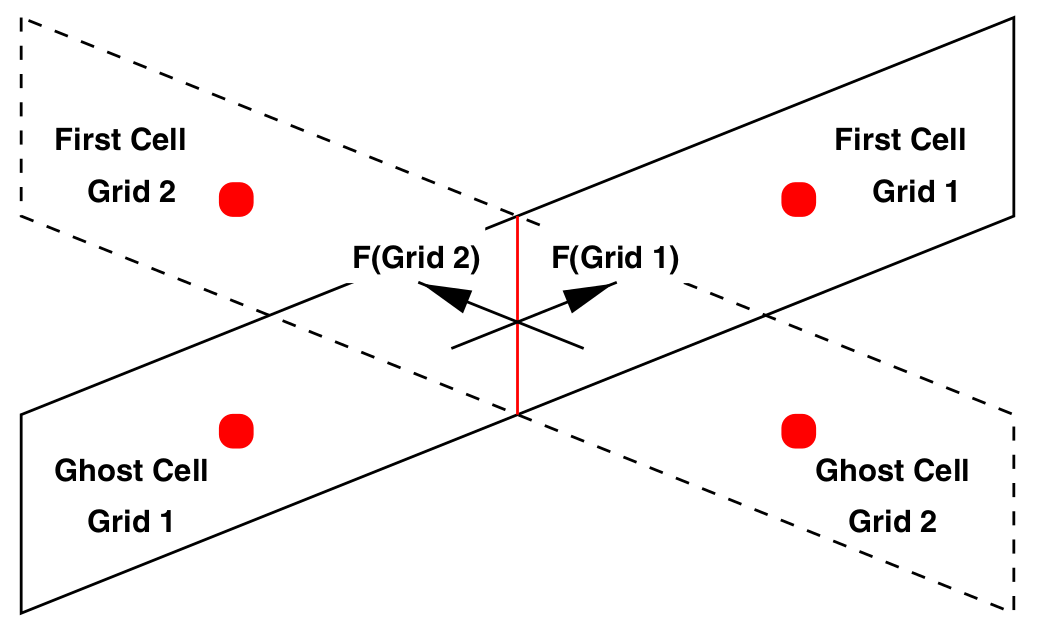
\includegraphics[width=0.5\linewidth]{flux_interface}
	\caption{Figure that illustrates the flux being computed twice on
		the cube edge, breaking the total mass conservation.
		Figure taken from \citet{ross:2006}.\label{chp5-fluxcube}}
\end{figure}
One common alternative used in the literature to handle the issue of values being defined twice at points on the
cube edges is to simply average the values (as seen in works such as \citet{ross:2006, chen:2008, chen:2021, mouallem:2023}).
When we are using flux averaging, we shall use the label \textbf{mf1}. When no mass fixer is used, we employ the label \textbf{mf0}.
 
\section{Numerical experiments}
\label{chp-cs-numexpadv}
This Section is dedicated to present the numerical experiments for the
advection equation on the sphere. In Table \ref{chp5-tab1} we present
the initial conditions (IC) and in Table \ref{chp5-tab2} we present
the velocity fields (VF) considered.
\begin{table}[!ht]
	\begin{tabular}{|c|l|l|}
		\hline
		IC name & \multicolumn{1}{c|}{$q_0$} \\ \hline
		IC1   & $\exp(b_0((X-X_0)^2+ (Y-Y_0)^2 + (Z-Z_0)^2))$ \\ \hline
		IC2   & $\exp(b_0[(X-X_1)^2+ (Y-Y_1)^2 + (Z-Z_1)^2] + \exp(b_0[(X-X_2)^2+ (Y-Y_2)^2 + (Z-Z_2)^2])$ \\ \hline
	\end{tabular}
	\caption{Initial conditions considered in the numerical experiments (Figure \ref{chp5-ic}).}
	\label{chp5-tab1} 
\end{table}

\begin{table}[!ht]
	\begin{tabular}{|c|l|l|l|}
		\hline
		VF name & \multicolumn{1}{c|}{$u_\lambda(\lambda,\phi,t) $} & \multicolumn{1}{c|}{$v_\phi(\lambda,\phi,t)$}  & \multicolumn{1}{c|}{$\Delta t^{(0)}$}\\ \hline
		VF1   & $u_0(\cos(\phi)\cos(\alpha) + \sin(\phi)\cos(\lambda)\sin(\alpha))$ 
		& $-u_0\sin(\lambda)\sin(\alpha)$ & 3600  \\ \hline
		VF2   & $u_0\sin^2(\lambda_p)\sin(2\phi)\cos(\frac{\pi t}{T})+u_0\cos\phi$ 
		& $u_0\sin(2\lambda_p)\cos(\phi)\cos(\frac{\pi t}{T})$& 1600  \\ \hline
		VF3   & $-u_0\sin^2(\frac{\lambda+\pi}{2})\sin(2\phi)\cos^2(\phi)\cos(\frac{\pi t}{T}),$ 
		& $\frac{u_0}{2}\sin(\lambda+\pi)\cos^3(\phi)\cos(\frac{\pi t}{T})$ & 7200 \\ \hline
	\end{tabular}
	\caption{Velocity fields considered in the numerical experiments and its initial time step $\Delta t^{(0)}$.}
	\label{chp5-tab2}
\end{table}
\begin{figure}[!htb]
	\centering
	\begin{subfigure}{0.45\textwidth}
		\centering
		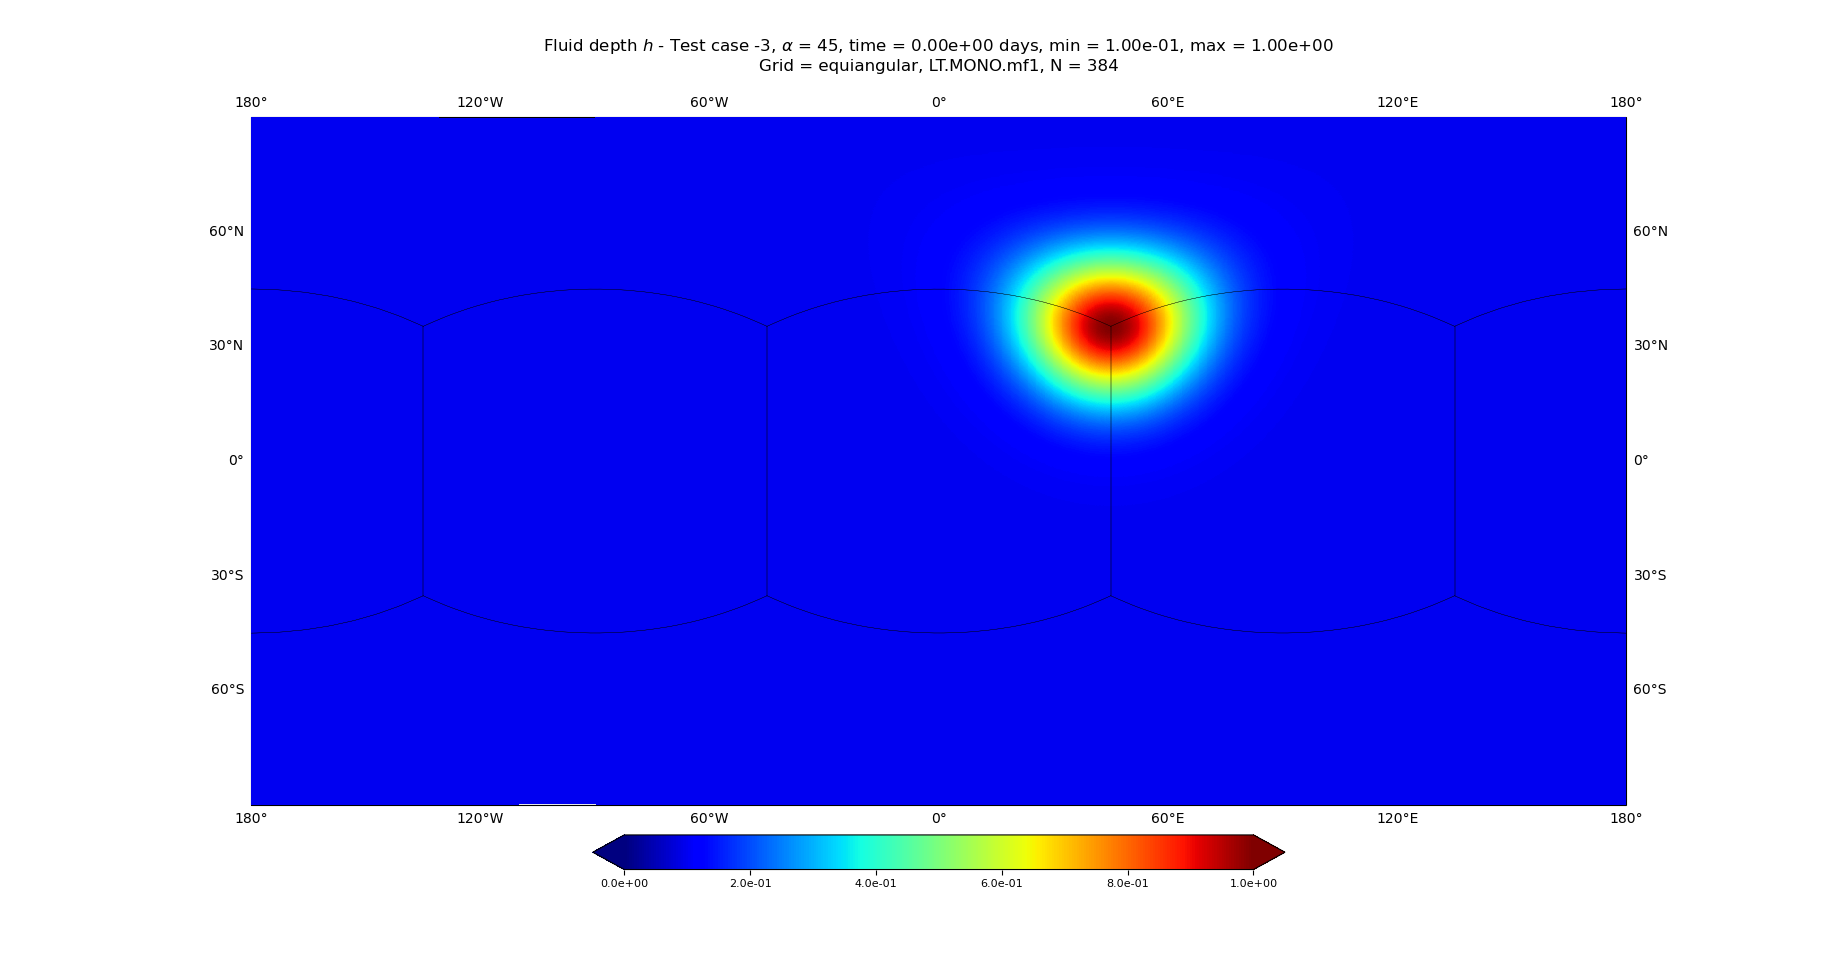
\includegraphics[width=1\linewidth]{h_tc-3_t0_alpha45_C384_g2_dg2_adv2_hord8_mf1_tf12}
		\caption{IC1. \label{chp5-ic1}}
	\end{subfigure}
	\begin{subfigure}{0.45\textwidth}
		\centering
		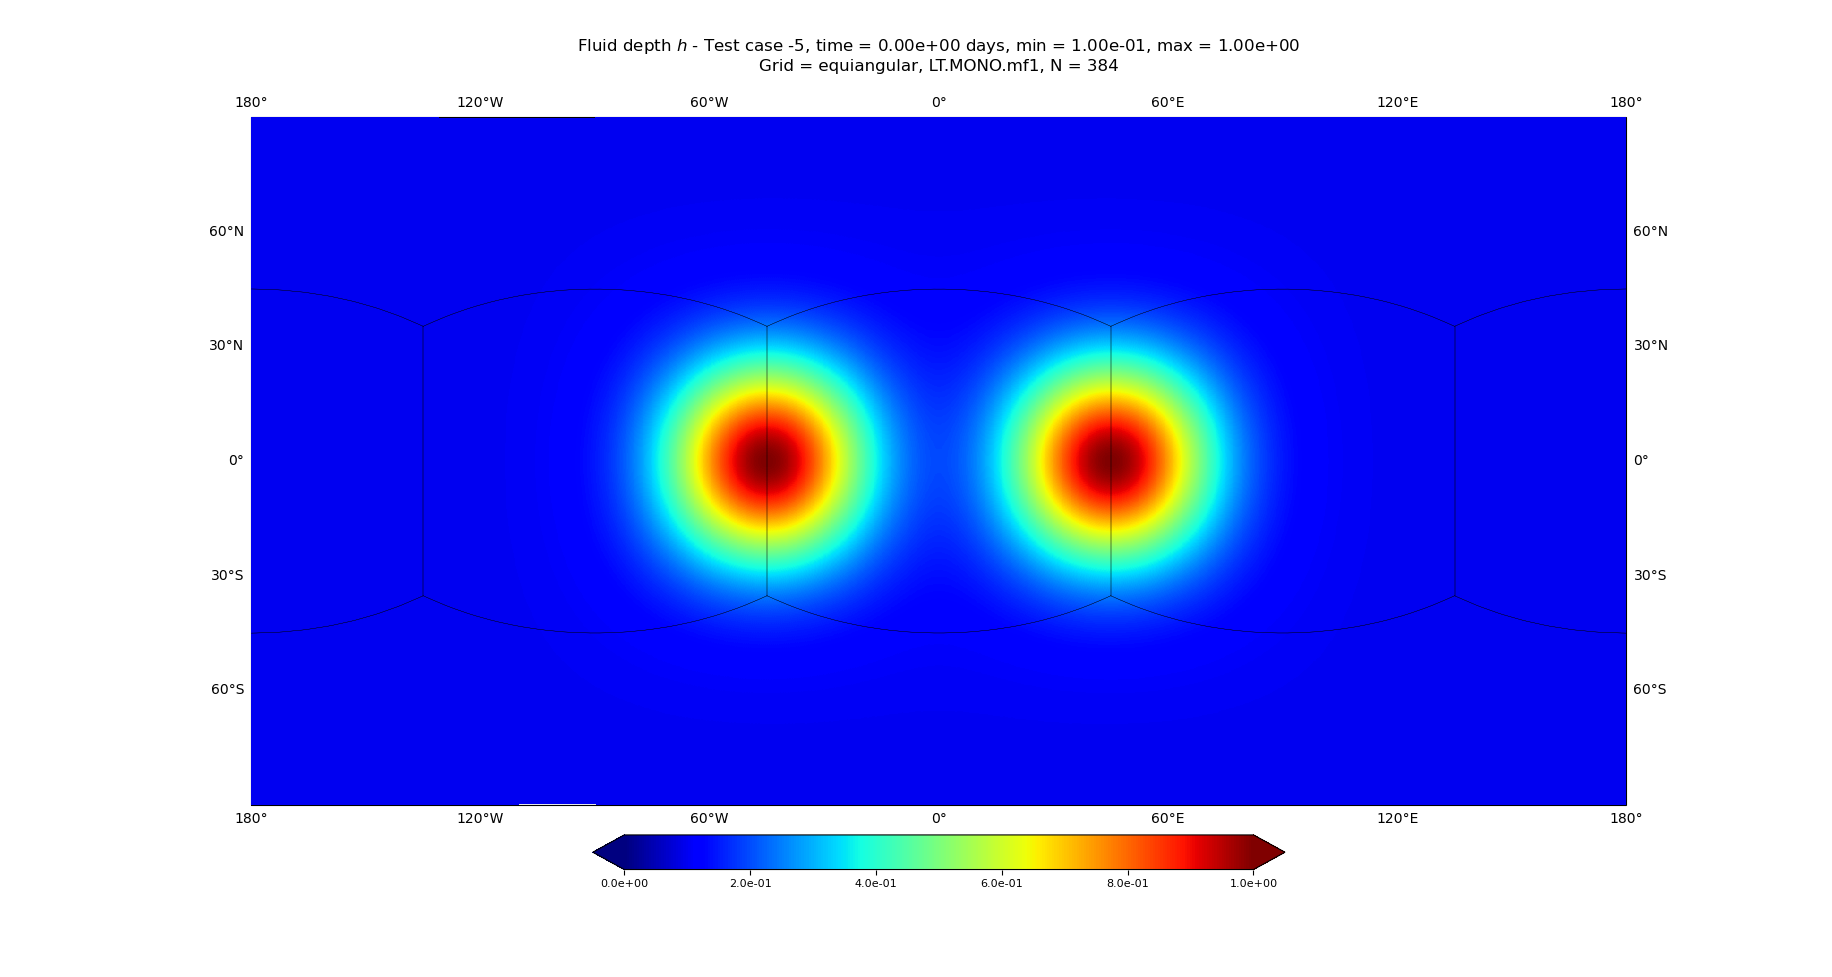
\includegraphics[width=1\linewidth]{h_tc-5_t0_alpha0_C384_g2_dg2_adv2_hord8_mf1_tf12}
		\caption{IC2. \label{chp5-ic2}}
	\end{subfigure}
	\caption{ Illustration of the initial conditions considered in this chapter (Table \ref{chp5-tab1}).\label{chp5-ic}}
\end{figure}


In Table \ref{chp5-tab1}, we have $(X_0,Y_0,Z_0)=(\frac{1}{\sqrt{3}},\frac{1}{\sqrt{3}},\frac{1}{\sqrt{3}})$, while 
$(X_1,Y_1,Z_1)$ and $(X_2,Y_2,Z_2)$ are the Cartesian coordinates of the latitude-longitude points
$(\lambda_1,\phi_1) = (-\frac{\pi}{4},0)$ and
$(\lambda_2,\phi_2) = ( \frac{\pi}{4},0)$, respectively.
IC1 represents a Gaussian hill centered at a cube corner and we set $b_0 = -10$.
IC2 represents two Gaussian hills as suggested by \citet{nair:2010} and we set $b_0 = -5$.
%IC3 is based on the steady flow presented in \citet{will:1992} and we adopt $\alpha=-\frac{45\pi}{180}$.
The initial conditions are shown in Figure \ref{chp5-ic}.

For the velocities provided in Table \ref{chp5-tab2}, we adopt the following parameter values: 
$\alpha=-\frac{45\pi}{180}$, $\lambda_p=\lambda-\frac{2\pi t}{T}$, $T=12$ days (12$\times$86400 seconds) and $R$ is the Earth radius.
For VF1 and VF2, we use $u_0 = \frac{2\pi R}{T}$, while for VF3, we use $u_0 = \frac{\pi R}{2T}$.
In this context, VF1 represents the non-divergent rotated zonal field introduced in \citet{will:1992}.
VF2 corresponds to the non-divergent deformational flow described in \citet{nair:2010},
and VF3 represents the divergent flow also presented in \citet{nair:2010}.
For all velocity fields presented here, the initial condition is equal to the final solution after 12 days.

We are going to consider the schemes LT-DP2 and PL-DP1 since these schemes yield better results on planar simulations (Section \ref{sec-ds-exp}).
For a shorter notation, we shall denote LT-DP2 and PL-DP1 by \textbf{LT} and \textbf{PL} advection schemes. 
These schemes will be tested using hord0 and hord8 1D PPM schemes.
As we mentioned in Section \ref{sec-metricppm}, the PL scheme needs the \textbf{mt1} 
metric term formulation for the 1D flux operators to eliminate the splitting error for a constant scalar field.
For the LT scheme, we shall use the \textbf{mt0} metric term formulation because for this scheme, 
we do not have the constraint of eliminating the splitting error for a constant scalar field. 
Furthermore, this formulation makes the LT scheme much more accurate, while \textbf{mt1} for LT makes it first-order.
We are also going to consider the simulations without mass fixer (\textbf{mf0}) and with flux averaging at
cube edges (\textbf{mf1}) to investigate the impact of flux averaging on accuracy.
Additionally, we are using the duo-grid to fill the ghost cell values.
The reader may refer to \citet{mouallem:2023} for a comparison between results on the duo-grid versus the kinked grid.
Both equi-edge (g0, Section \ref{cs-equiedge}) and equiangular grids (g2, Section \ref{cs-equiangular}) are going to be consider in this Section.

To compute the convergence, consider cubed-sphere grids with value of $N_k =  48\times2^{k}$,
and $\Delta t^{(k)} = \frac{\Delta t^{(k)}}{2^k}$, $k=0, \ldots, 4$, where
the value of $\Delta t^{(0)}$ in Table \ref{chp5-tab2} for each VF.
The relative error in the maximum norm is computed as
\begin{equation}
	E_k = \frac{\max |q^{N_T} - q^0|}{\max {|q^0|}},
\end{equation}
and the convergence rate is defined as
\begin{equation*}
	CR_k = \frac{\ln{\bigg(\frac{E_{k}}{E_{k-1}}}\bigg)}{\ln 2}, \quad \text{for} \quad k = 1, \ldots 4.
\end{equation*}

\newpage
\subsection{Advection of one Gaussian hill through the rotated zonal wind}
As a second test case, we consider the advection of the Gaussian hill given by IC1 using 
the rotated zonal wind VF1.
\begin{figure}[!htb]
	\centering
	\begin{subfigure}{0.45\textwidth}
		\centering
		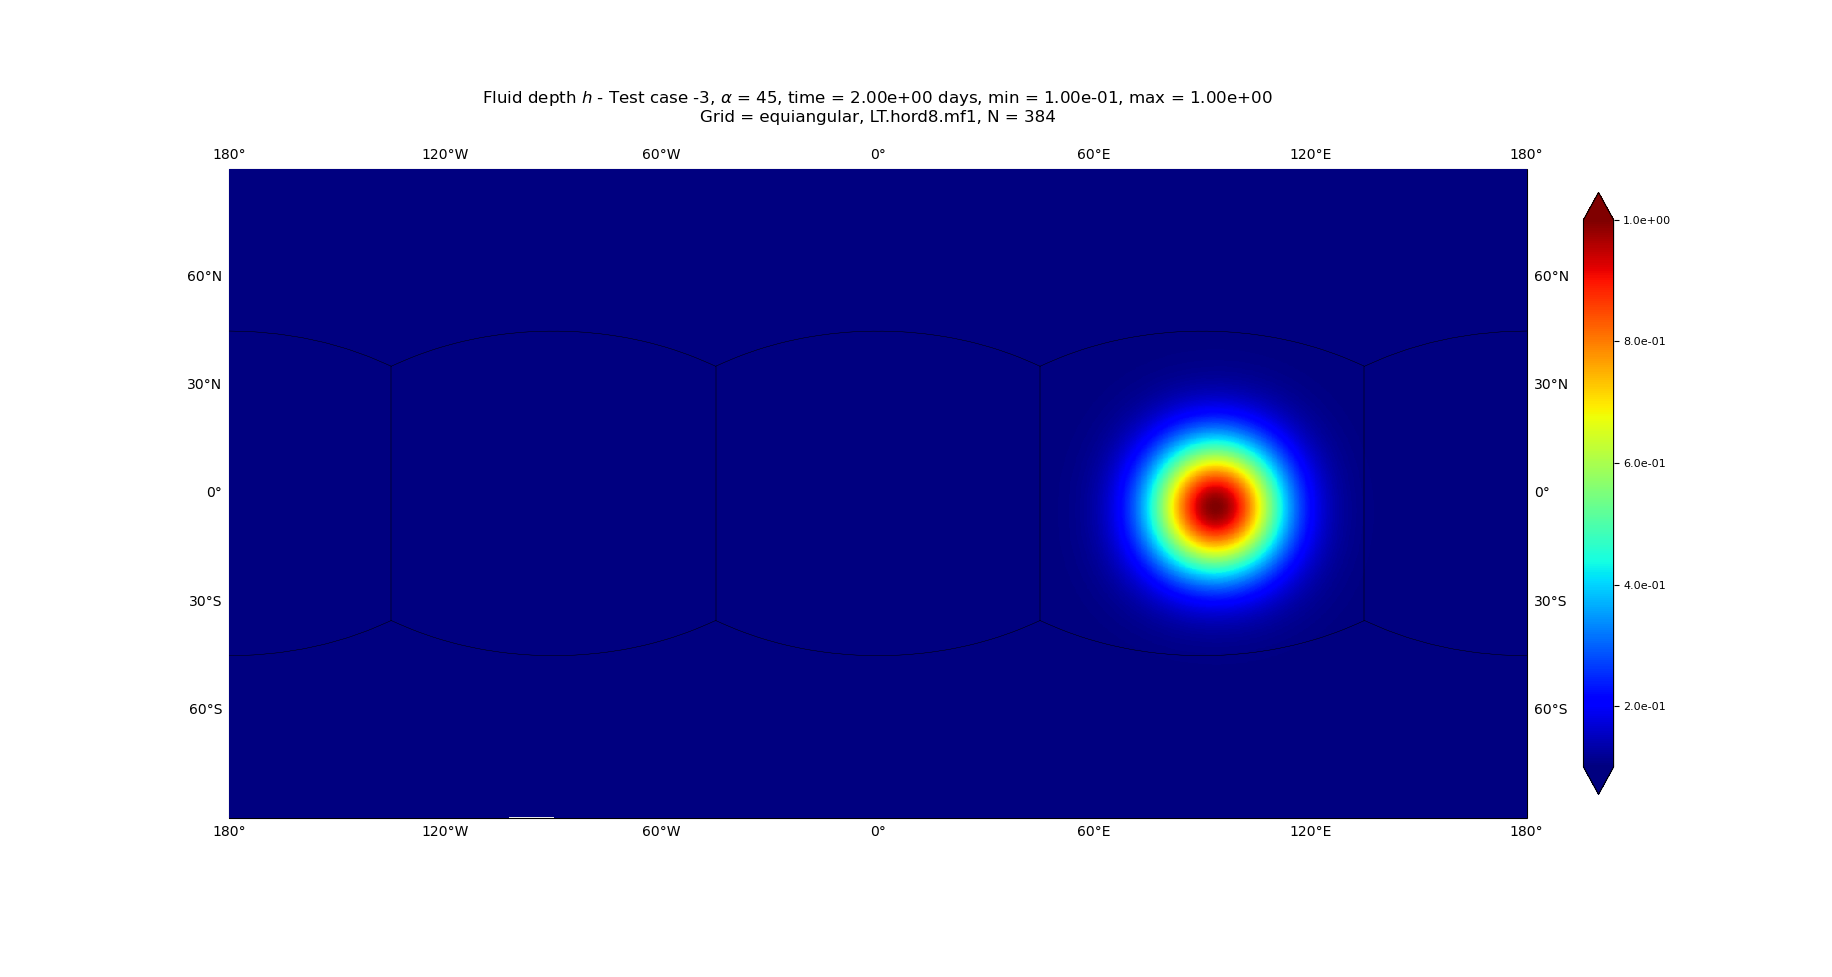
\includegraphics[width=1\linewidth]{h_tc-3_t2_alpha45_C384_g2_dg2_adv2_hord8_mf1_tf12}
		\caption{$t=2$ days.\label{chp-advcs-sec-exp-adv2-a}}
	\end{subfigure}
	\begin{subfigure}{0.45\textwidth}
		\centering
		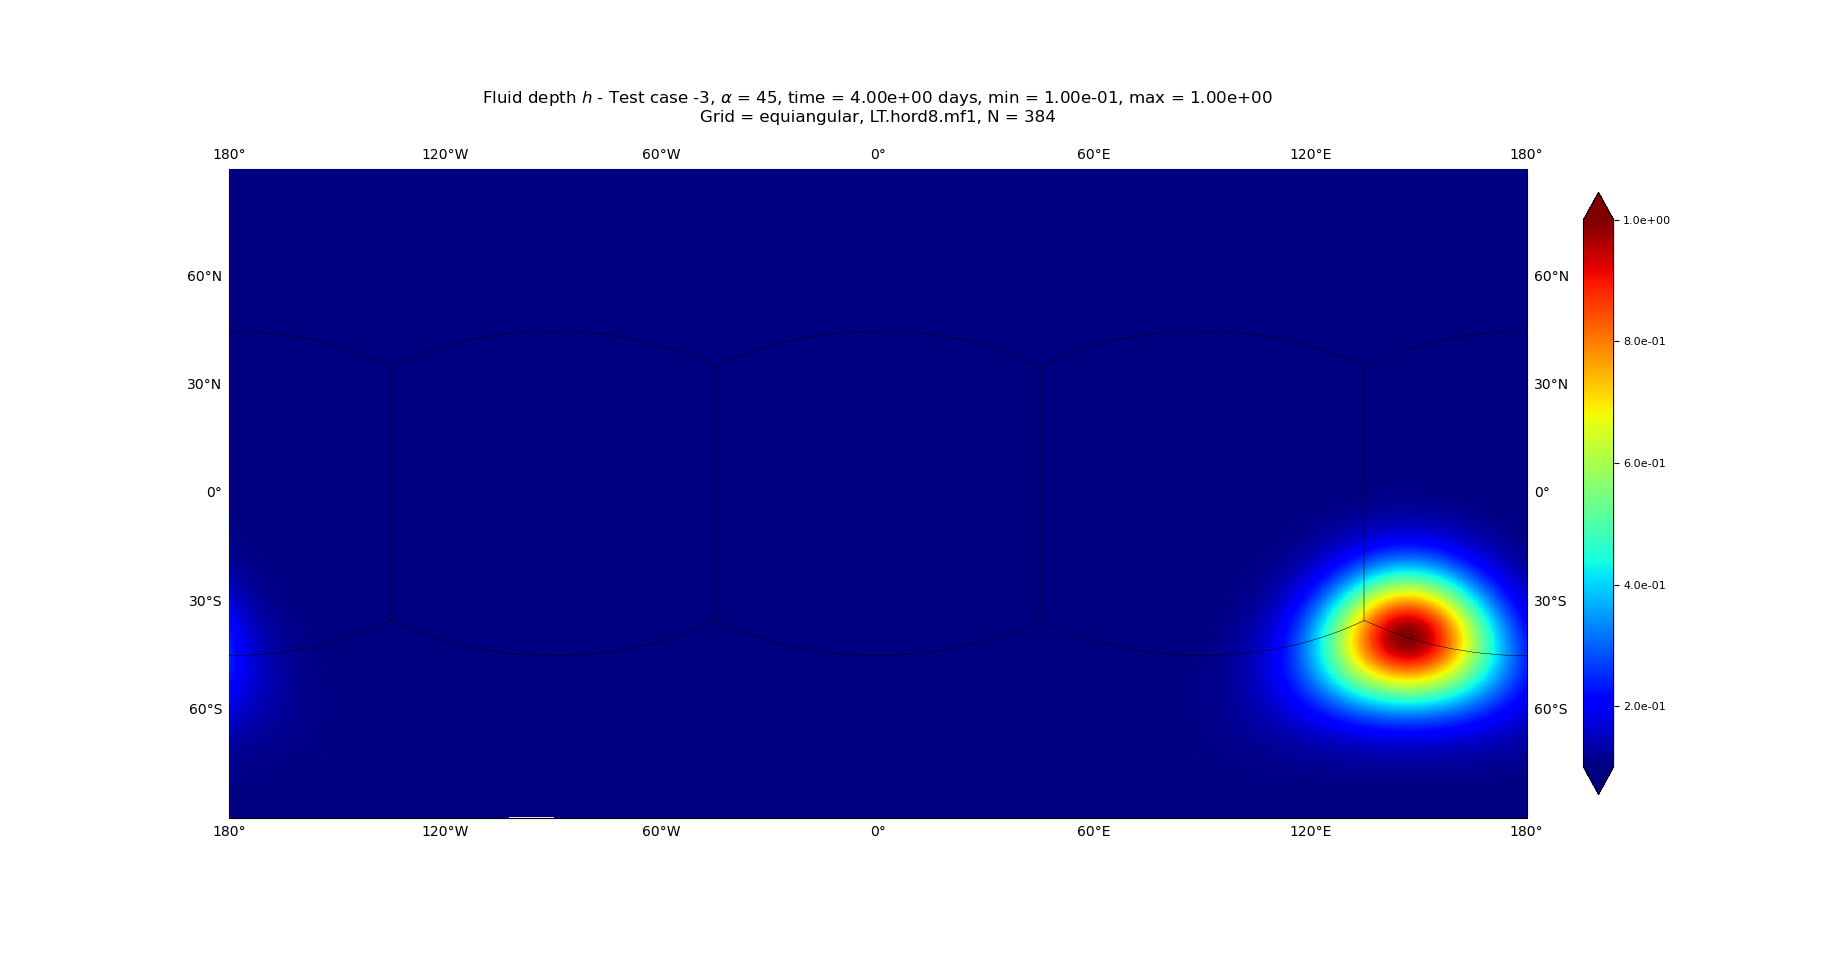
\includegraphics[width=1\linewidth]{h_tc-3_t4_alpha45_C384_g2_dg2_adv2_hord8_mf1_tf12}
		\caption{$t=4$ days.\label{chp-advcs-sec-exp-adv2-b}}
	\end{subfigure}

	\begin{subfigure}{0.45\textwidth}
		\centering
		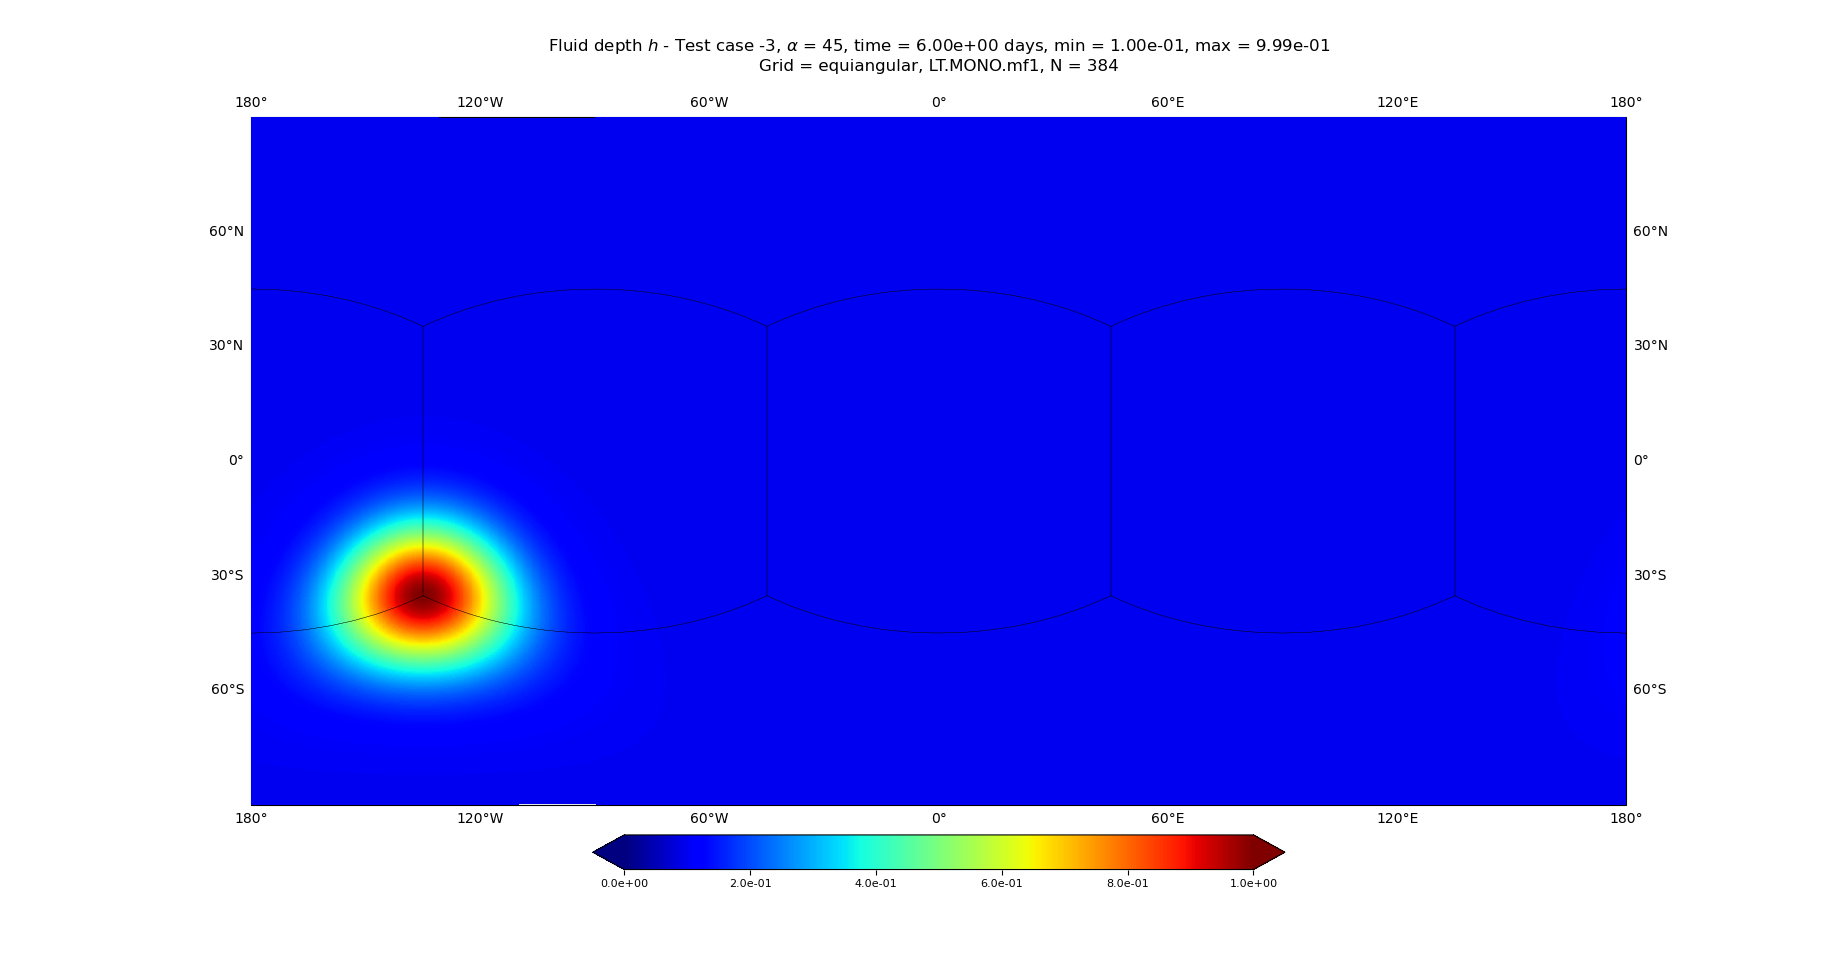
\includegraphics[width=1\linewidth]{h_tc-3_t6_alpha45_C384_g2_dg2_adv2_hord8_mf1_tf12}
		\caption{$t=6$ days.\label{chp-advcs-sec-exp-adv2-c}}
	\end{subfigure}	
	\begin{subfigure}{0.45\textwidth}
		\centering
		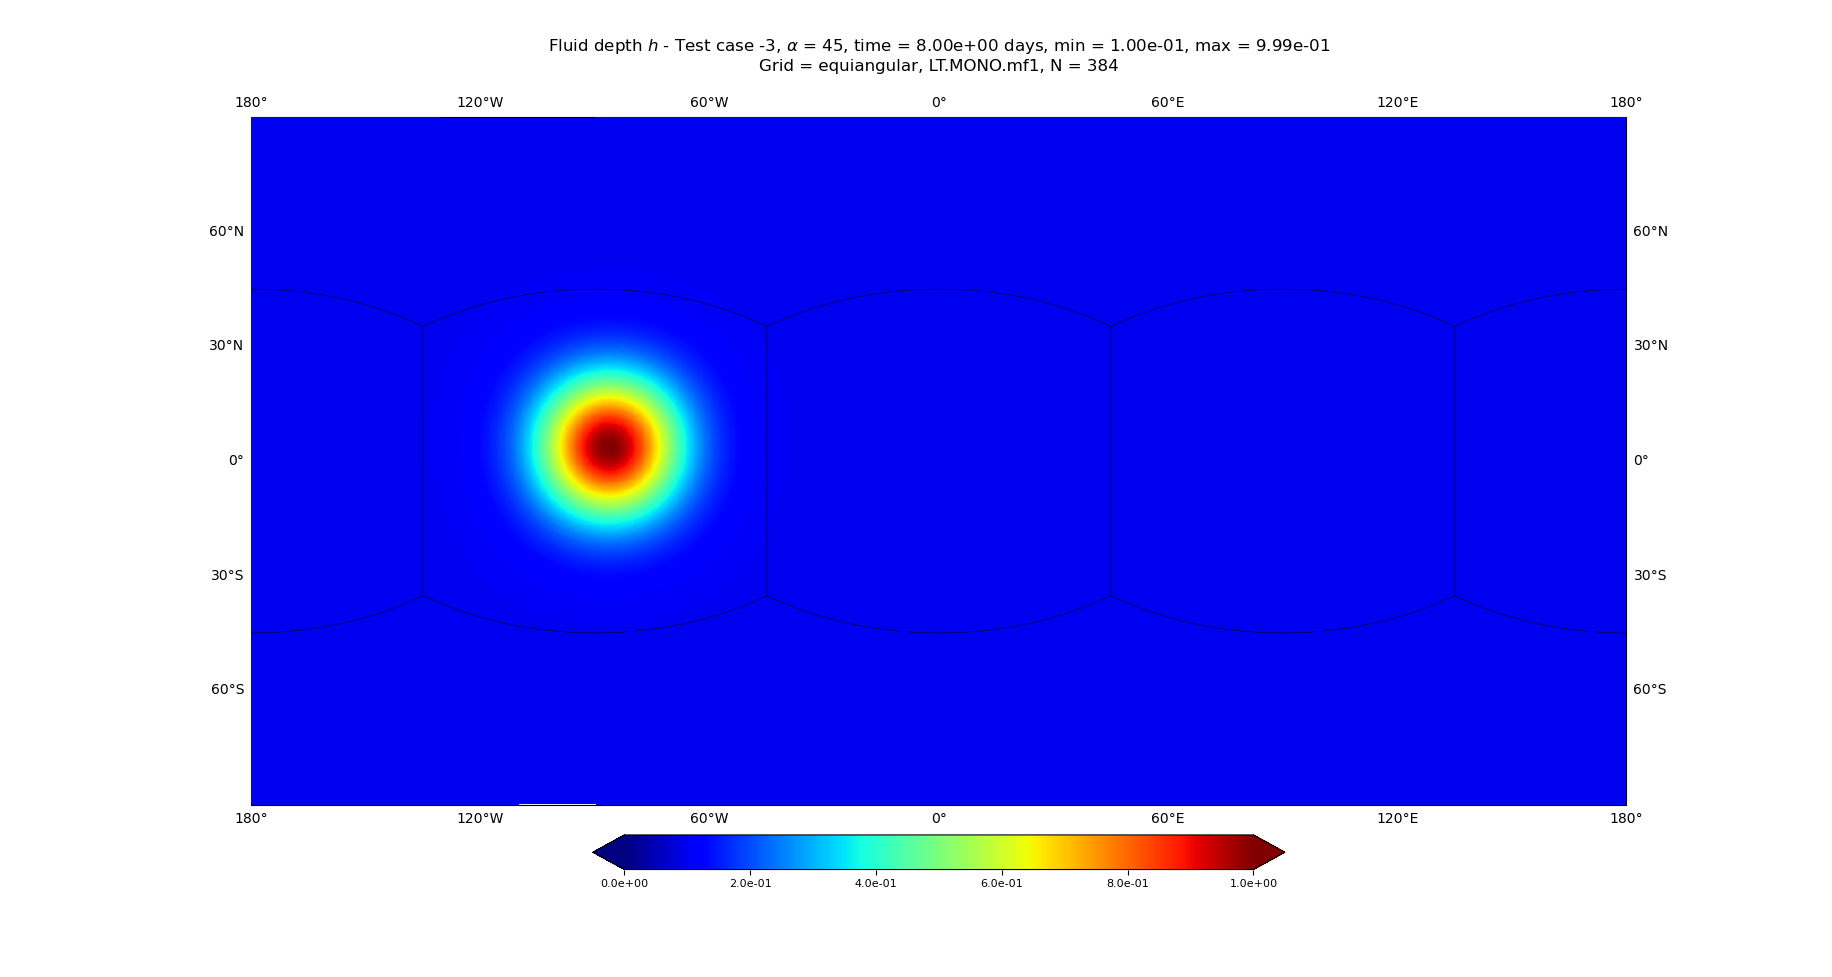
\includegraphics[width=1\linewidth]{h_tc-3_t8_alpha45_C384_g2_dg2_adv2_hord8_mf1_tf12}
		\caption{$t=8$ days.\label{chp-advcs-sec-exp-adv2-d}}
	\end{subfigure}

	\begin{subfigure}{0.45\textwidth}
		\centering
		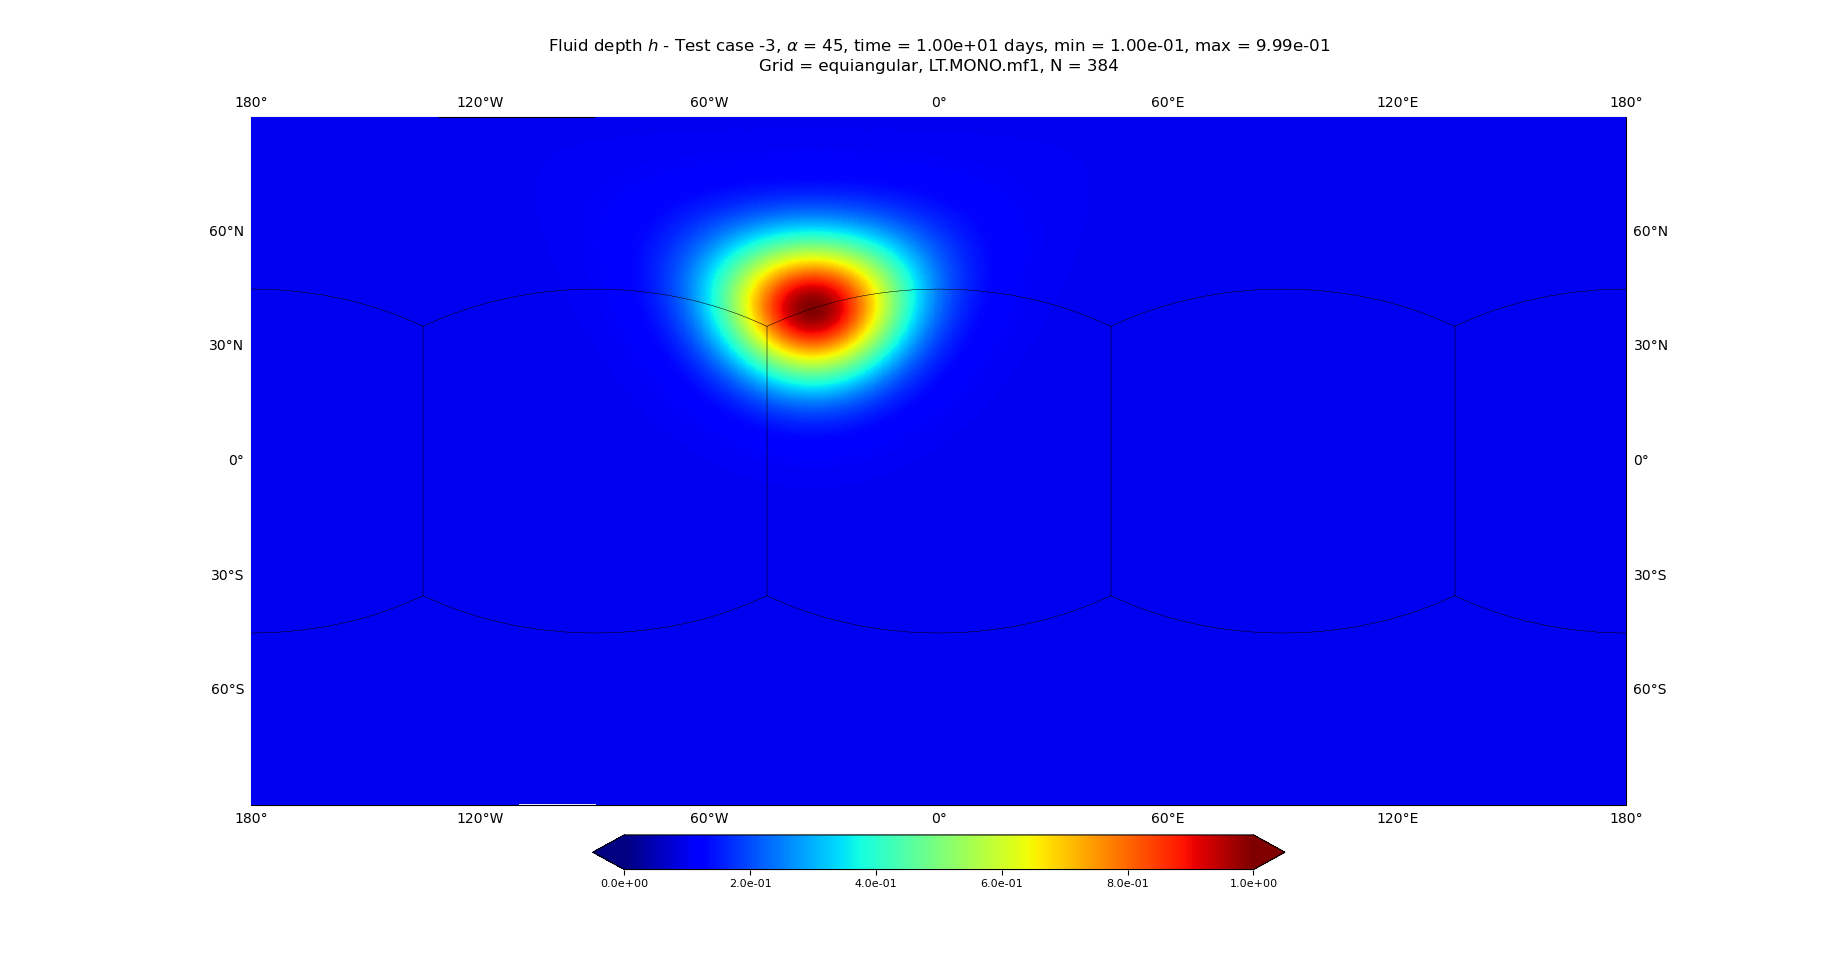
\includegraphics[width=1\linewidth]{h_tc-3_t10_alpha45_C384_g2_dg2_adv2_hord8_mf1_tf12}
		\caption{$t=10$ days.\label{chp-advcs-sec-exp-adv2-e}}
	\end{subfigure}
	\begin{subfigure}{0.45\textwidth}
		\centering
		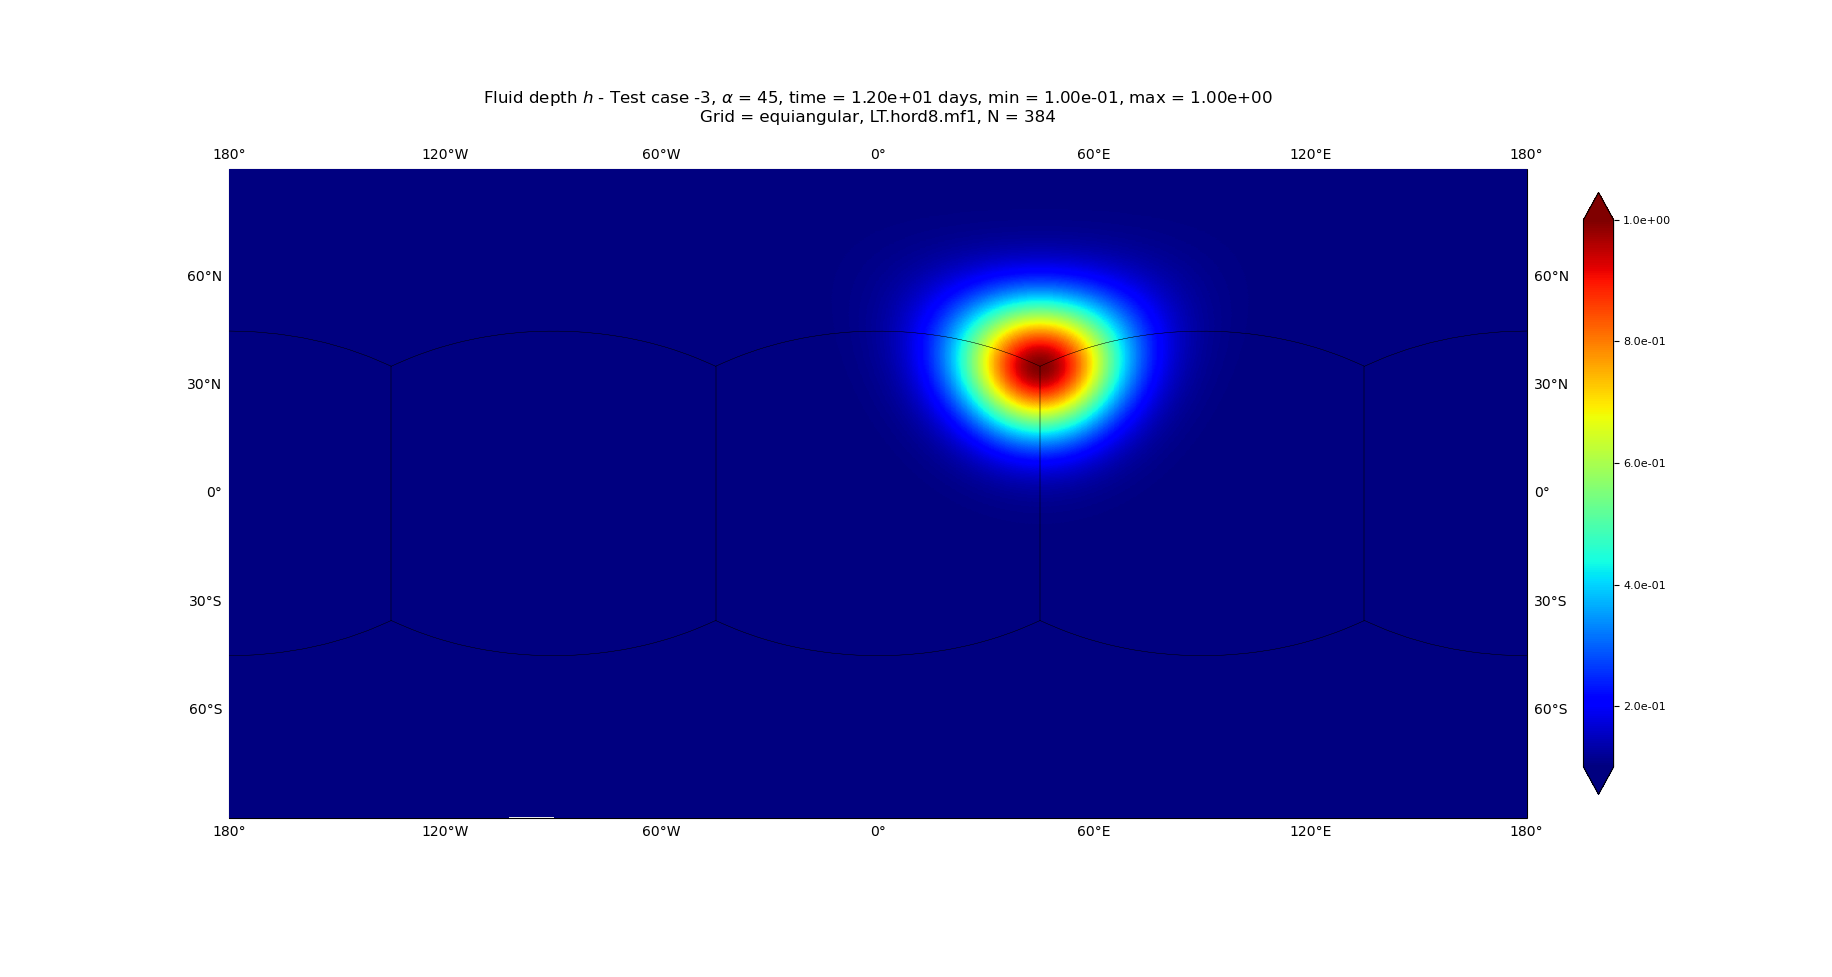
\includegraphics[width=1\linewidth]{h_tc-3_t12_alpha45_C384_g2_dg2_adv2_hord8_mf1_tf12}
		\caption{$t=12$ days.\label{chp-advcs-sec-exp-adv2-f}}
	\end{subfigure}
	\caption{Advection experiment  results using IC1 and VF1 from Table \ref{chp5-ic}.
		These figures show the advected profile at
		2 \eqref{chp-advcs-sec-exp-adv2-a}, 
		4  \eqref{chp-advcs-sec-exp-adv2-b},
		6  \eqref{chp-advcs-sec-exp-adv2-c},
		8  \eqref{chp-advcs-sec-exp-adv2-d},
		10  \eqref{chp-advcs-sec-exp-adv2-e},
		and 12  \eqref{chp-advcs-sec-exp-adv2-f} days.
		We are using the LT-hord8-mf1 scheme on the g2 grid with $N=384$. \label{chp-advcs-sec-exp-adv2}}
\end{figure}

\newpage
\begin{figure}[!htb]
	\centering
	\begin{subfigure}{0.45\textwidth}
		\centering
		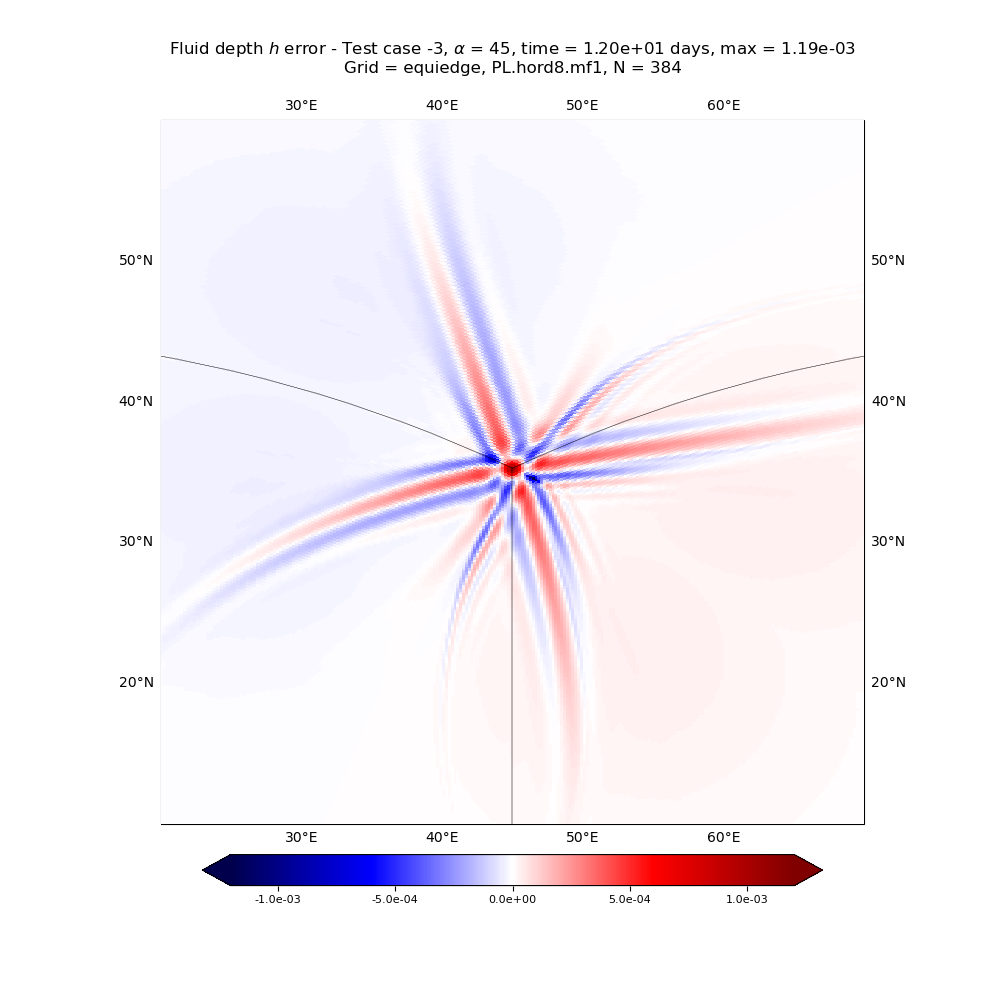
\includegraphics[width=1\linewidth]{h_error_tc-3_t12_alpha45_C384_g0_dg2_adv1_hord8_mf1_tf12}
		\caption{PL scheme.\label{chp-advcs-sec-exp-adv2-errors-0a}}
	\end{subfigure}
	\begin{subfigure}{0.45\textwidth}
		\centering
		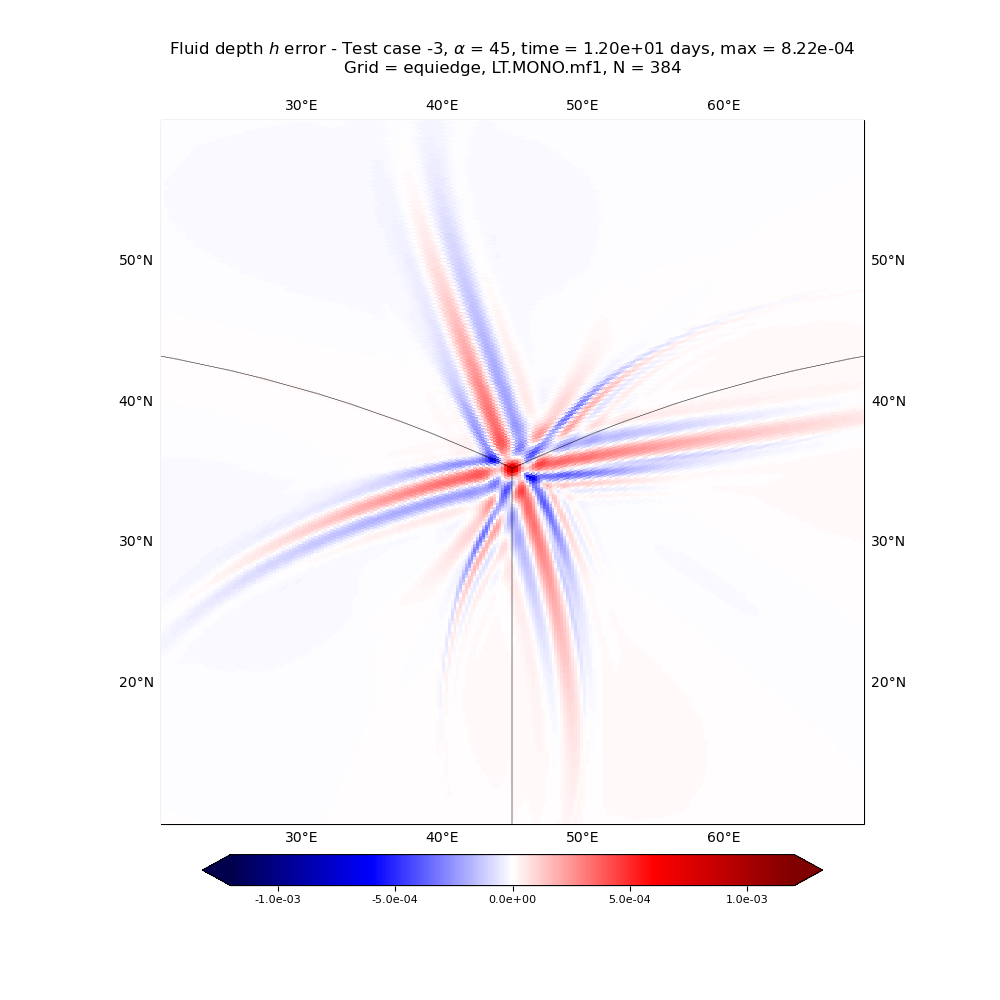
\includegraphics[width=1\linewidth]{h_error_tc-3_t12_alpha45_C384_g0_dg2_adv2_hord8_mf1_tf12}
		\caption{LT scheme.\label{chp-advcs-sec-exp-adv2-errors-0b}}
	\end{subfigure}
	\caption{
		Advection experiment errors at a cube corner using IC1 and VF1 from Table \ref{chp5-ic} after 12 days, using hord8
		with PL (left) and LT schemes (right) on the g0 grid with $N=384$. 
		\label{chp-advcs-sec-exp-adv2-errors-0}}
\end{figure}
\begin{figure}[!htb]
	\centering
	\begin{subfigure}{0.45\textwidth}
		\centering
		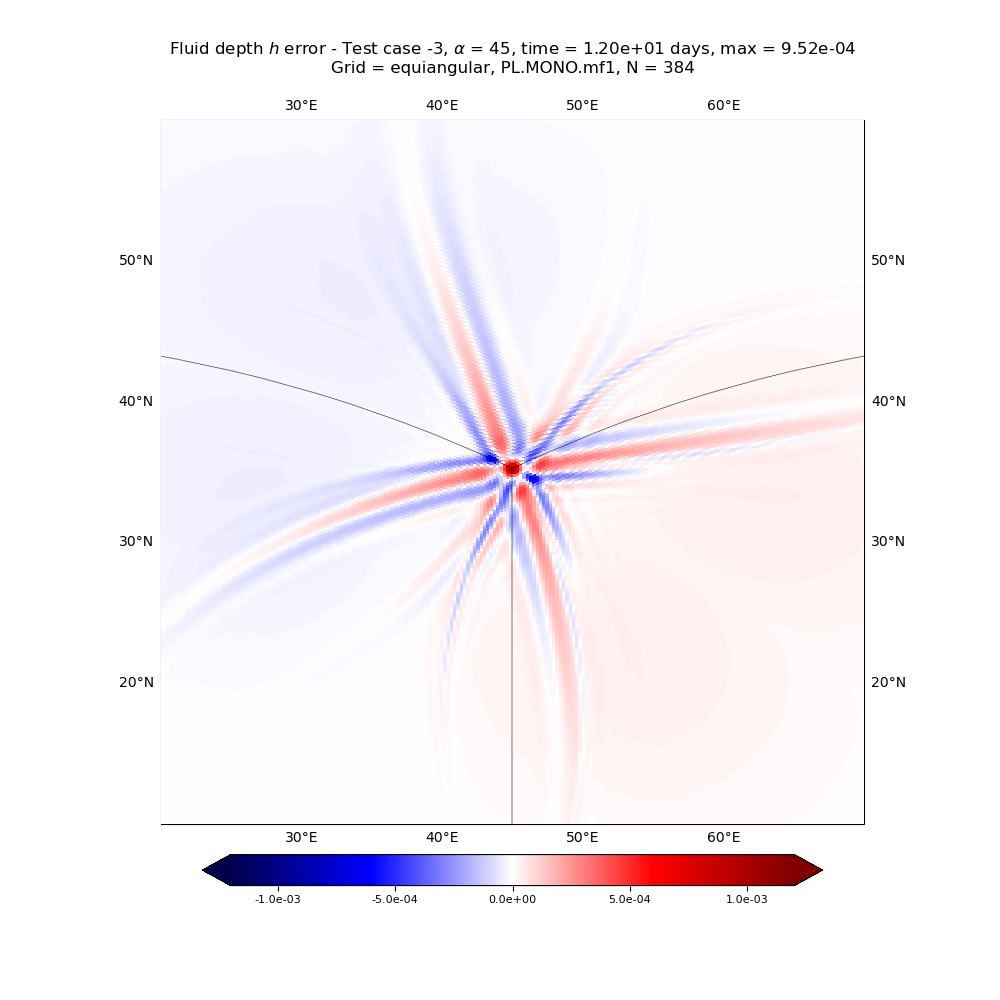
\includegraphics[width=1\linewidth]{h_error_tc-3_t12_alpha45_C384_g2_dg2_adv1_hord8_mf1_tf12}
		\caption{PL scheme.\label{chp-advcs-sec-exp-adv2-errors-2a}}
	\end{subfigure}
	\begin{subfigure}{0.45\textwidth}
		\centering
		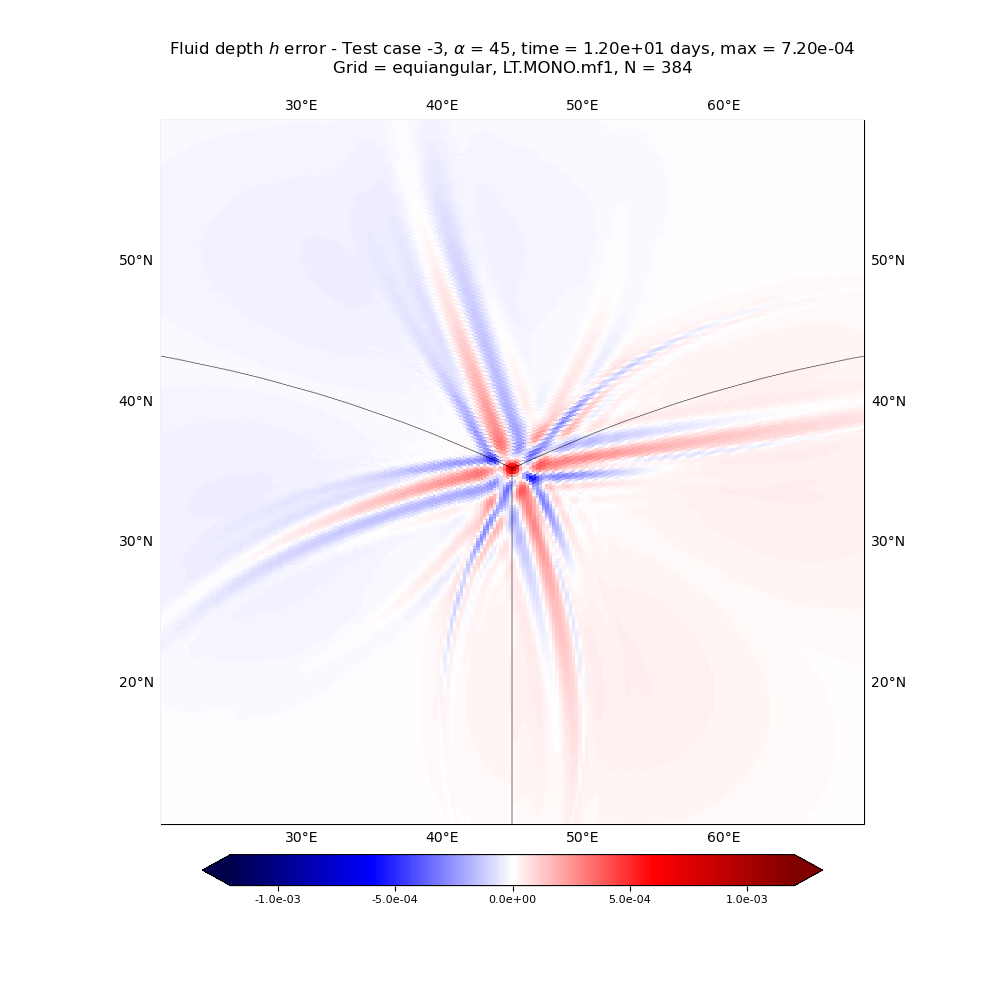
\includegraphics[width=1\linewidth]{h_error_tc-3_t12_alpha45_C384_g2_dg2_adv2_hord8_mf1_tf12}
		\caption{LT scheme.\label{chp-advcs-sec-exp-adv2-errors-2b}}
	\end{subfigure}
	\caption{As Figure \ref{chp-advcs-sec-exp-adv2-errors-0} but using the g2 grid.\label{chp-advcs-sec-exp-adv2-errors-2}}
\end{figure}

\newpage
\begin{figure}[!htb]
		\centering
		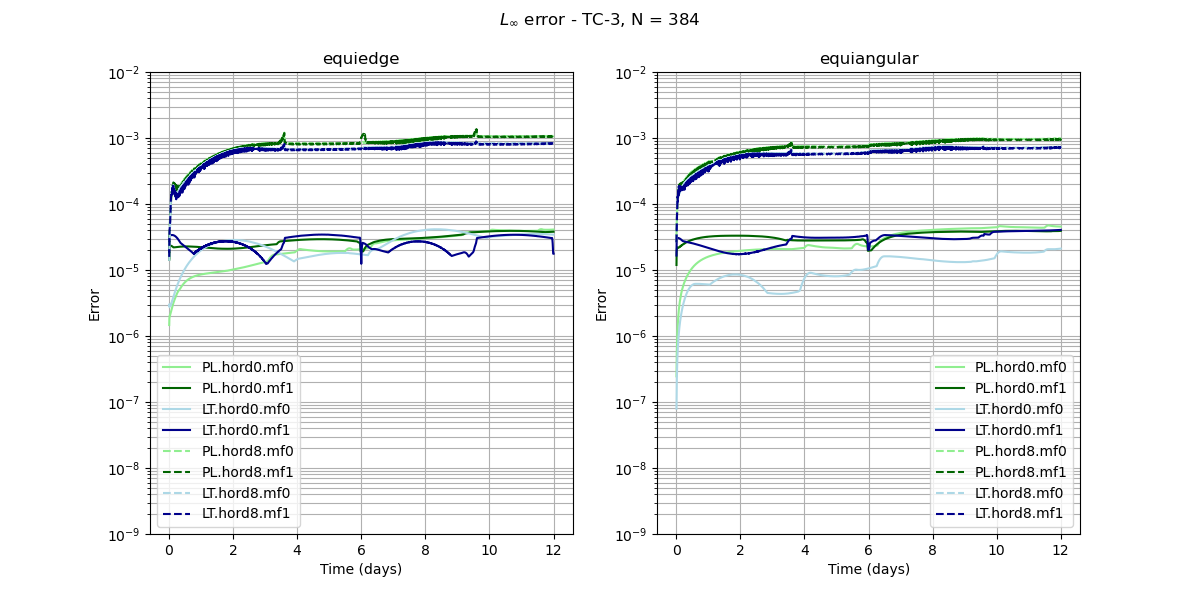
\includegraphics[width=1\linewidth]{tc-3_C384_linf_errors}
		\caption{
$L_{\infty}$ error evolution for IC1 and VF1 from Table \ref{chp5-ic} on the g0 (left) and g2 (right) grids for 12 days.
Blue lines indicate the use of the LT scheme, while green lines represent the PL scheme.
Solid lines represent the results with the hord8 scheme, whereas dashed lines represent the results with hord8.
Light colors show the result without mass fixer (mf0), whereas dark colors show the results with flux averaging (mf1).\label{chp-advcs-sec-exp-adv2-evol-linf}}
\end{figure}

\begin{figure}[!htb]
		\centering
		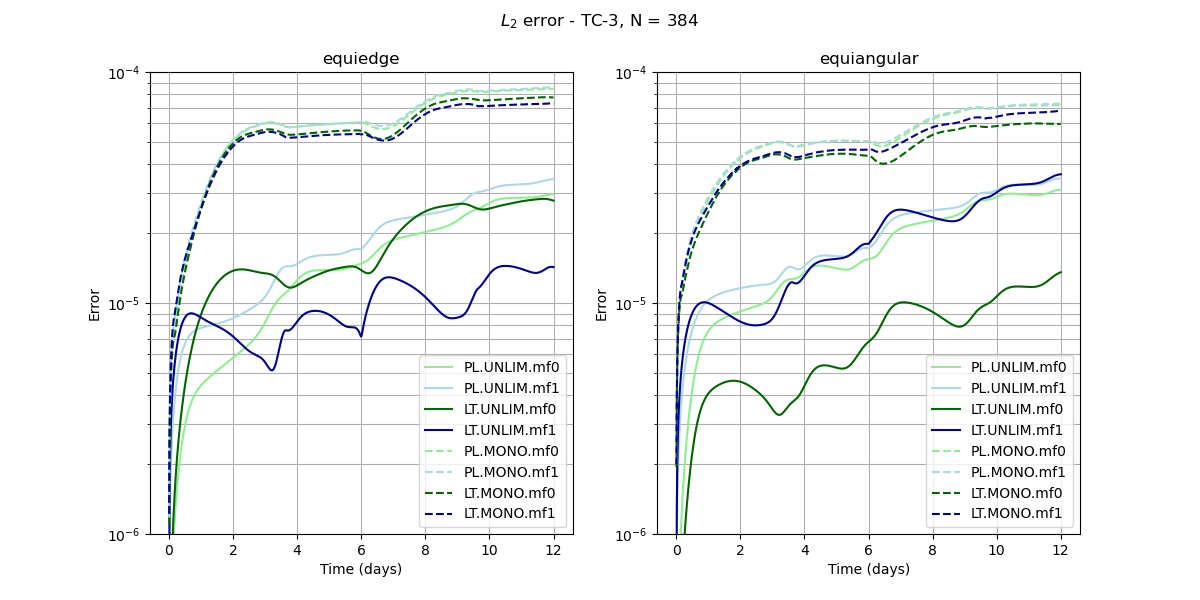
\includegraphics[width=1\linewidth]{tc-3_C384_l2_errors}
		\caption{As Figure \ref{chp-advcs-sec-exp-adv2-evol-linf} but using the $L_2$ error.\label{chp-advcs-sec-exp-adv2-evol-l2}}
\end{figure}

\newpage
\begin{figure}[!htb]
	\centering
	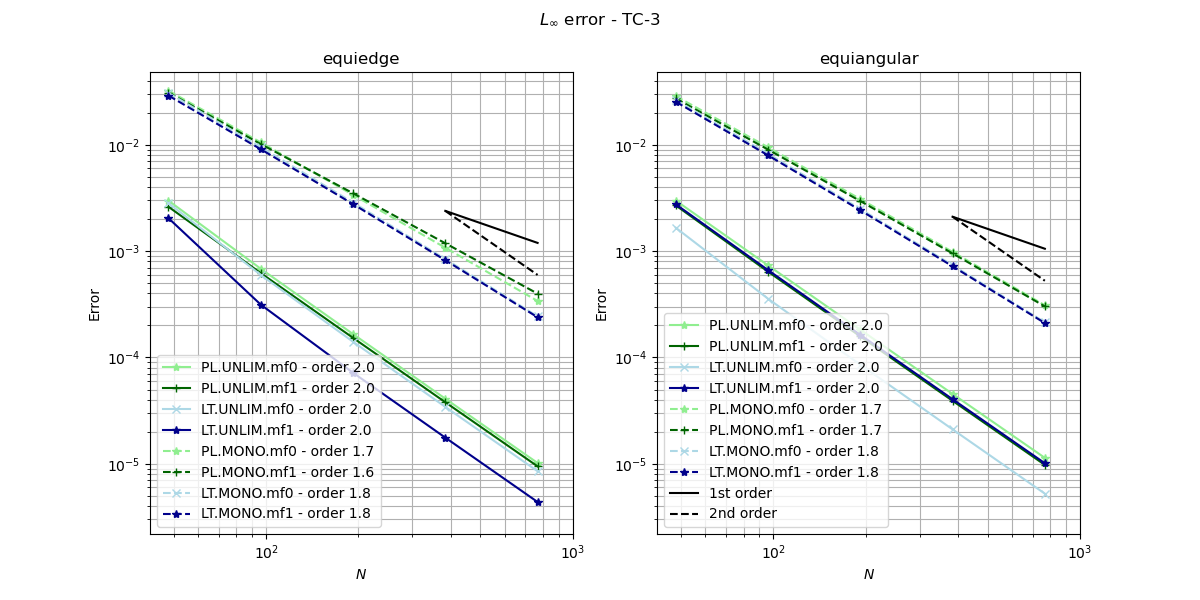
\includegraphics[width=1\linewidth]{linferror_tc-3_alpha45}
	\caption{
$L_{\infty}$ error convergence for IC1 and VF1 from Table \ref{chp5-ic} on the g0 (left) and g2 (right) grids after 12 days.
Blue lines indicate the use of the LT scheme, while green lines represent the PL scheme.
Solid lines represent the results with the hord8 scheme, whereas dashed lines represent the results with hord8.
Light colors show the result without mass fixer (mf0), whereas dark colors show the results with flux averaging (mf1).\label{chp-advcs-sec-exp-adv2-linf}}
\end{figure}

\begin{figure}[!htb]
	\centering
	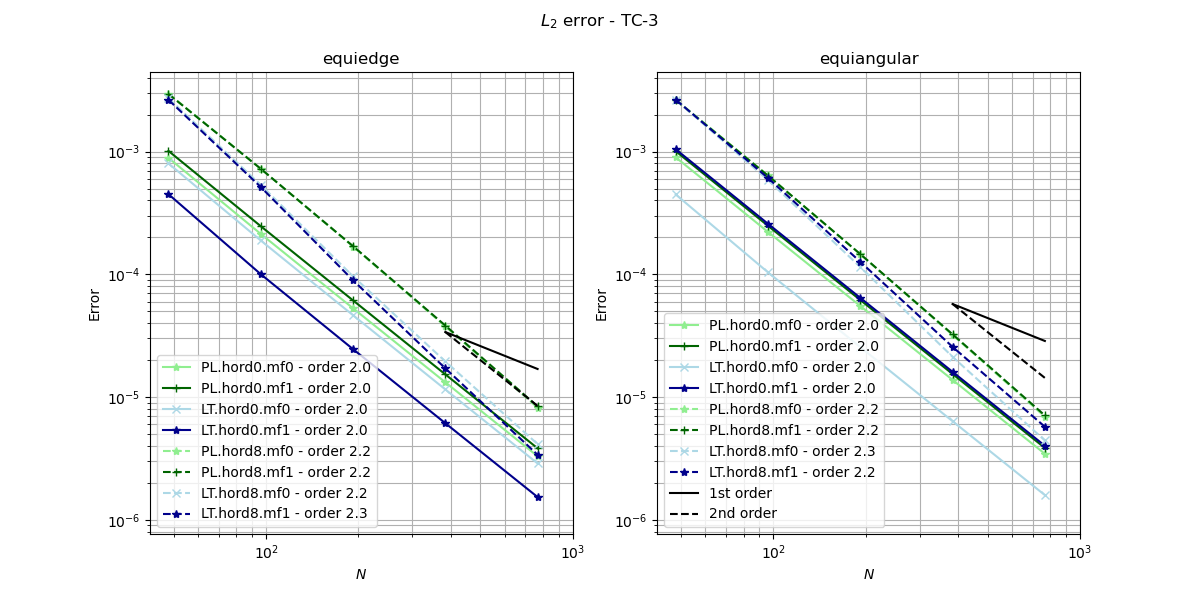
\includegraphics[width=1\linewidth]{l2error_tc-3_alpha45}
	\caption{As Figure \ref{chp-advcs-sec-exp-adv2-linf} but considering the $L_2$ norm. \label{chp-advcs-sec-exp-adv2-error}}
\end{figure}

\newpage
\subsection{Non-divergent deformational flow}
As the fourth test case, we considered the non-divergent vector field VF2 velocity from table \ref{chp5-tab2}. 
We used the initial condition IC2 from table \ref{chp5-tab1}, as suggested by \citet{nair:2010}, which also shows how the solution evolves with time. 
\begin{figure}[!htb]
	\centering
	\begin{subfigure}{0.45\textwidth}
		\centering
		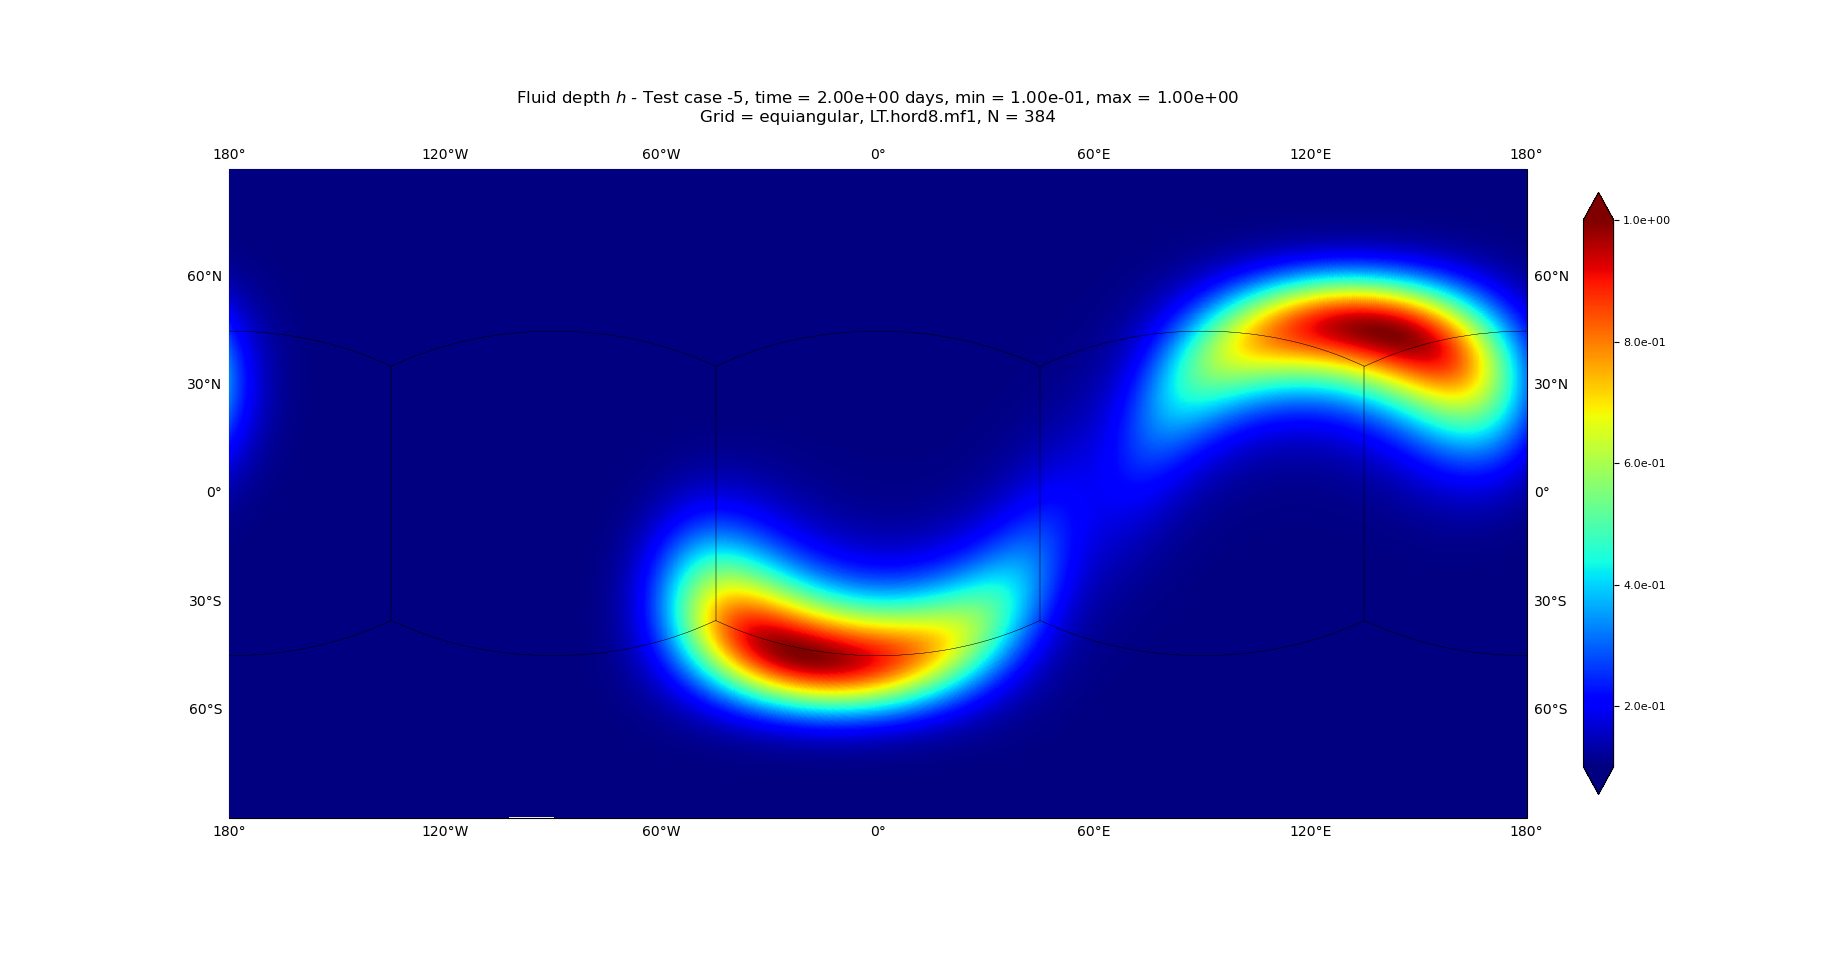
\includegraphics[width=1\linewidth]{h_tc-5_t2_alpha0_C384_g2_dg2_adv2_hord8_mf1_tf12}
		\caption{$t=2$ days.\label{chp-advcs-sec-exp-adv3-a}}
	\end{subfigure}
	\begin{subfigure}{0.45\textwidth}
		\centering
		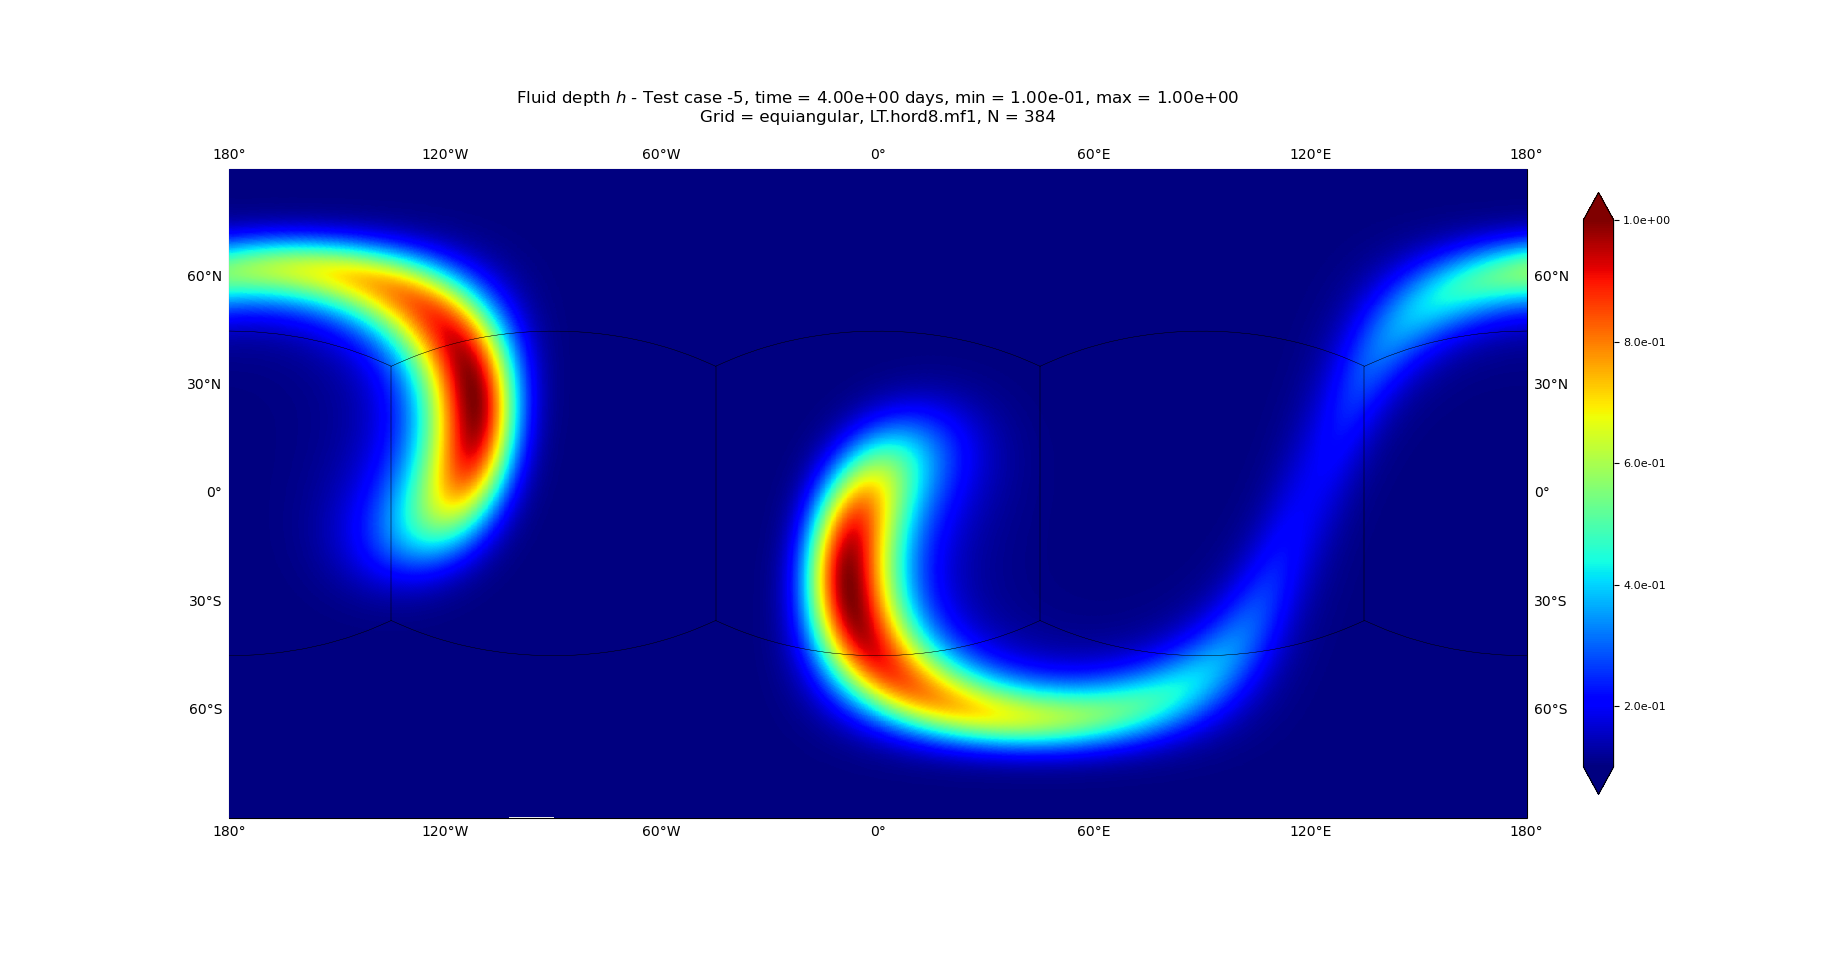
\includegraphics[width=1\linewidth]{h_tc-5_t4_alpha0_C384_g2_dg2_adv2_hord8_mf1_tf12}
		\caption{$t=4$ days.\label{chp-advcs-sec-exp-adv3-b}}
	\end{subfigure}

	\begin{subfigure}{0.45\textwidth}
		\centering
		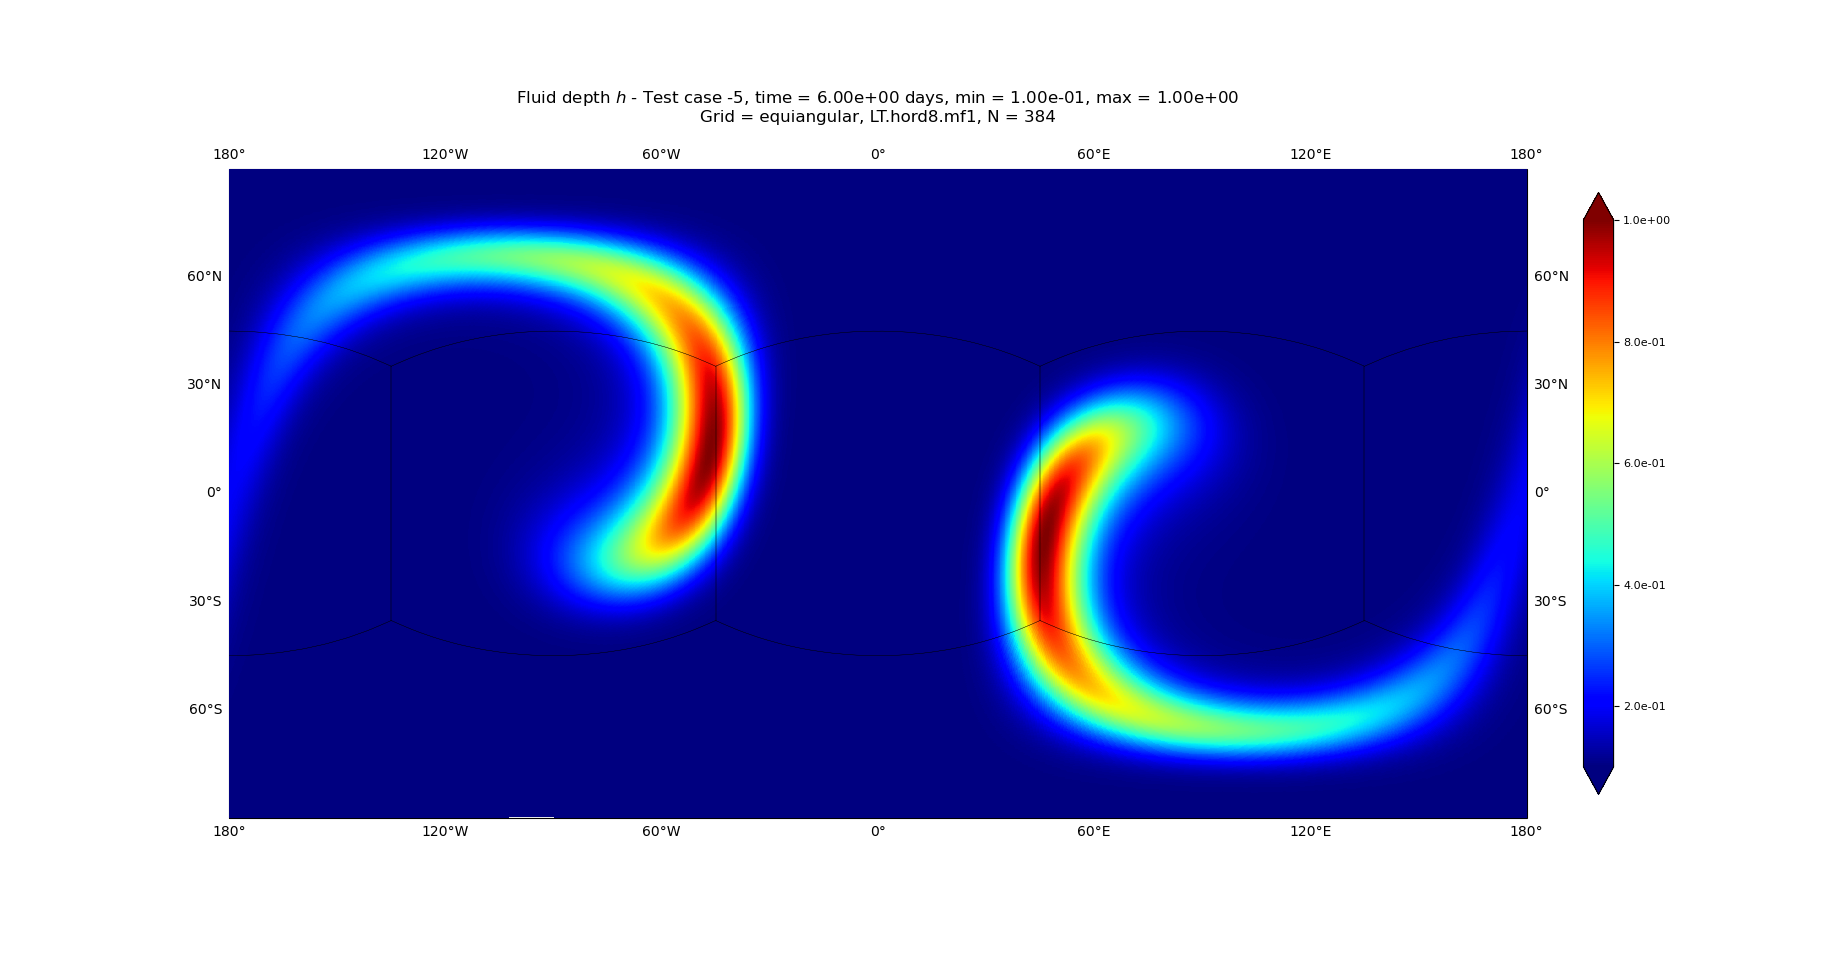
\includegraphics[width=1\linewidth]{h_tc-5_t6_alpha0_C384_g2_dg2_adv2_hord8_mf1_tf12}
		\caption{$t=6$ days.\label{chp-advcs-sec-exp-adv3-c}}
	\end{subfigure}
	\begin{subfigure}{0.45\textwidth}
		\centering
		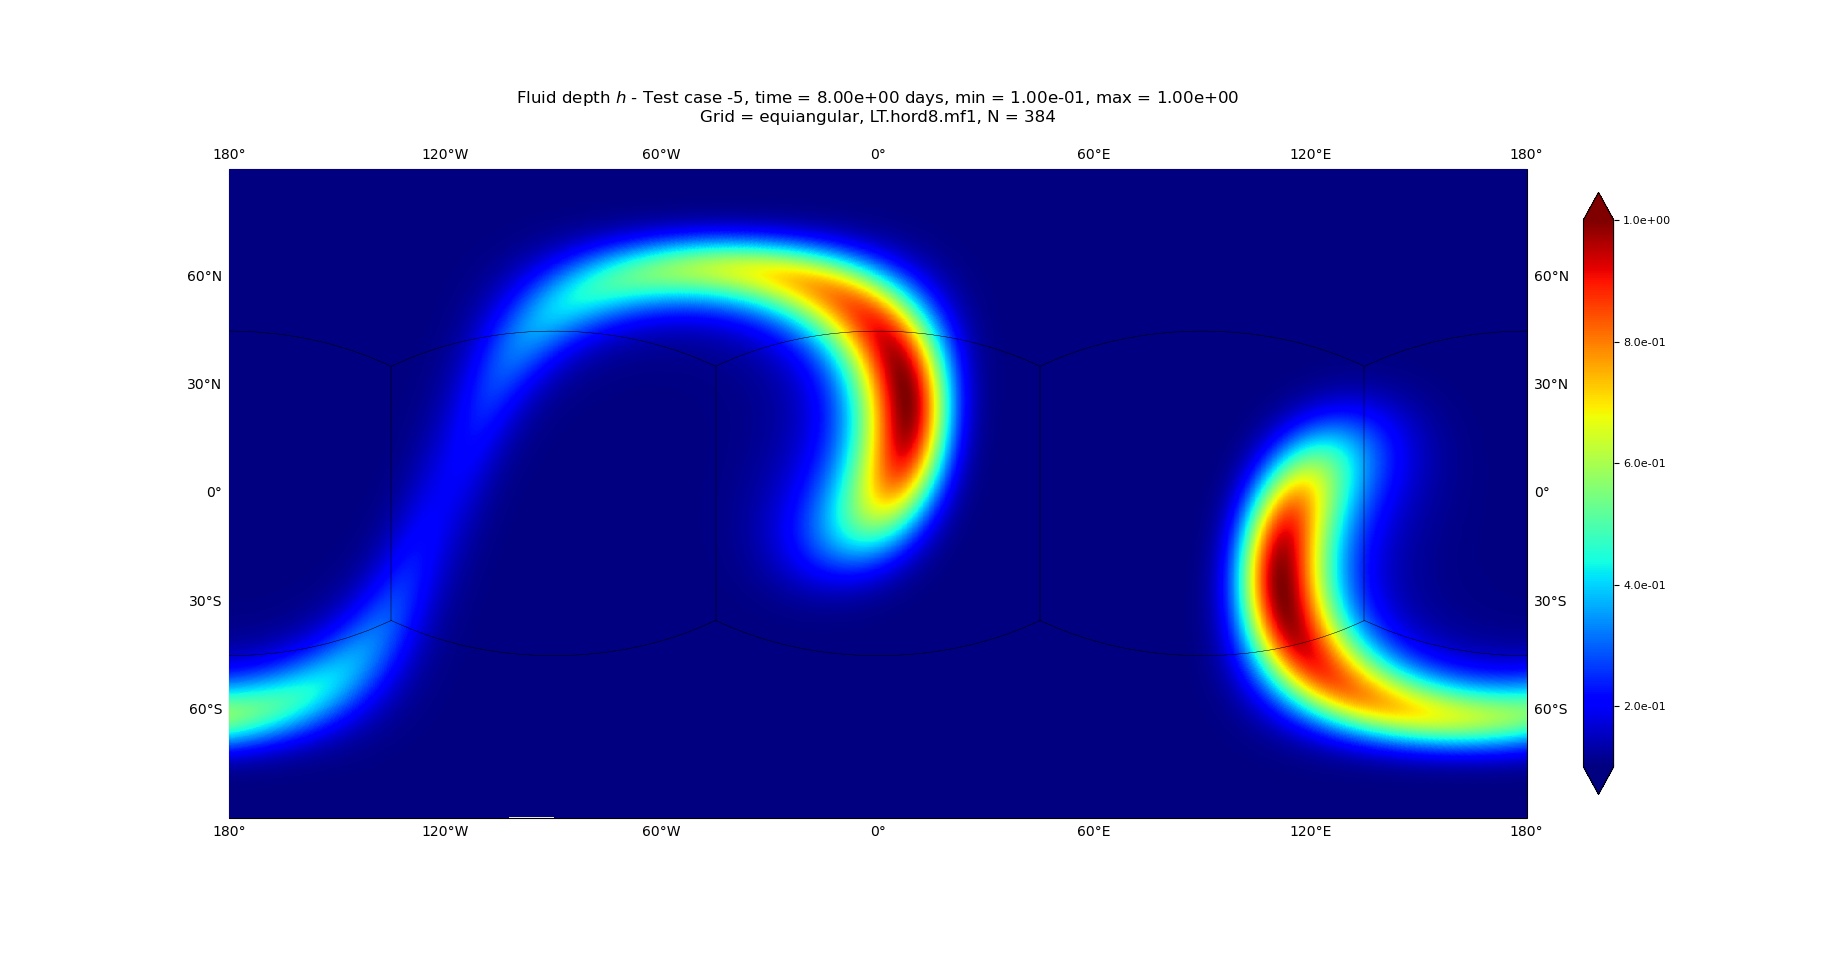
\includegraphics[width=1\linewidth]{h_tc-5_t8_alpha0_C384_g2_dg2_adv2_hord8_mf1_tf12}
		\caption{$t=8$ days.\label{chp-advcs-sec-exp-adv3-d}}
	\end{subfigure}

	\begin{subfigure}{0.45\textwidth}
		\centering
		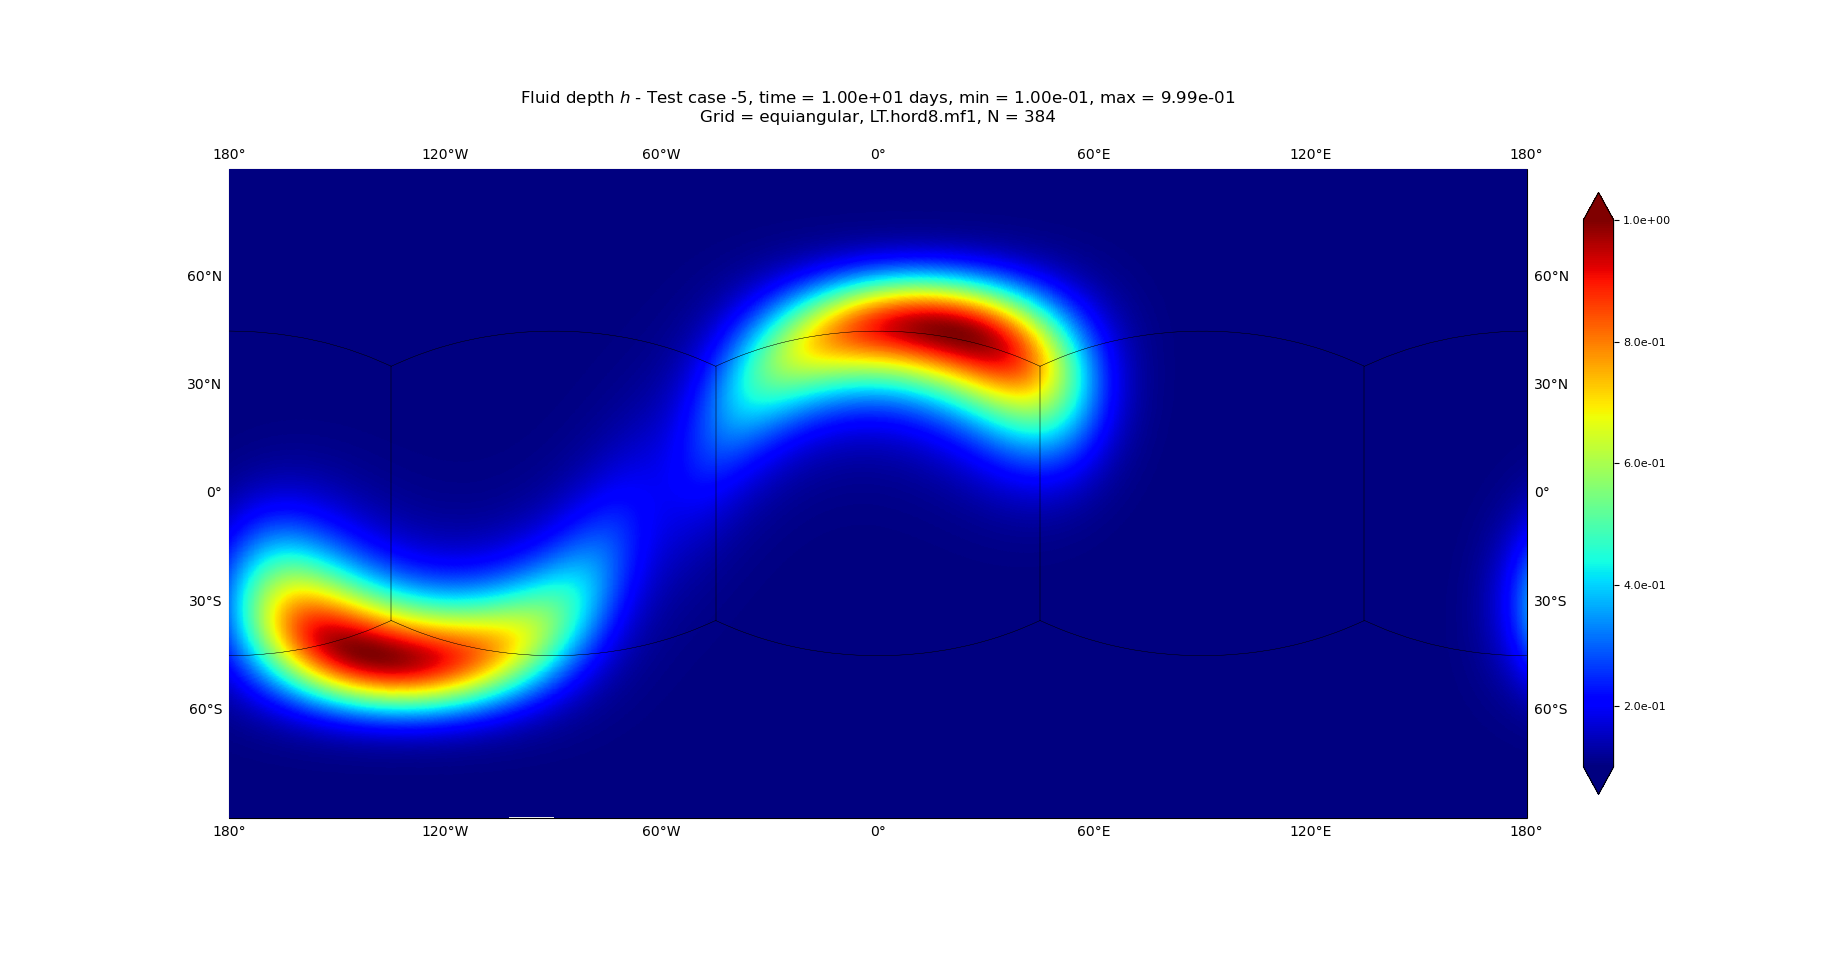
\includegraphics[width=1\linewidth]{h_tc-5_t10_alpha0_C384_g2_dg2_adv2_hord8_mf1_tf12}
		\caption{$t=10$ days.\label{chp-advcs-sec-exp-adv3-e}}
	\end{subfigure}
	\begin{subfigure}{0.45\textwidth}
		\centering
		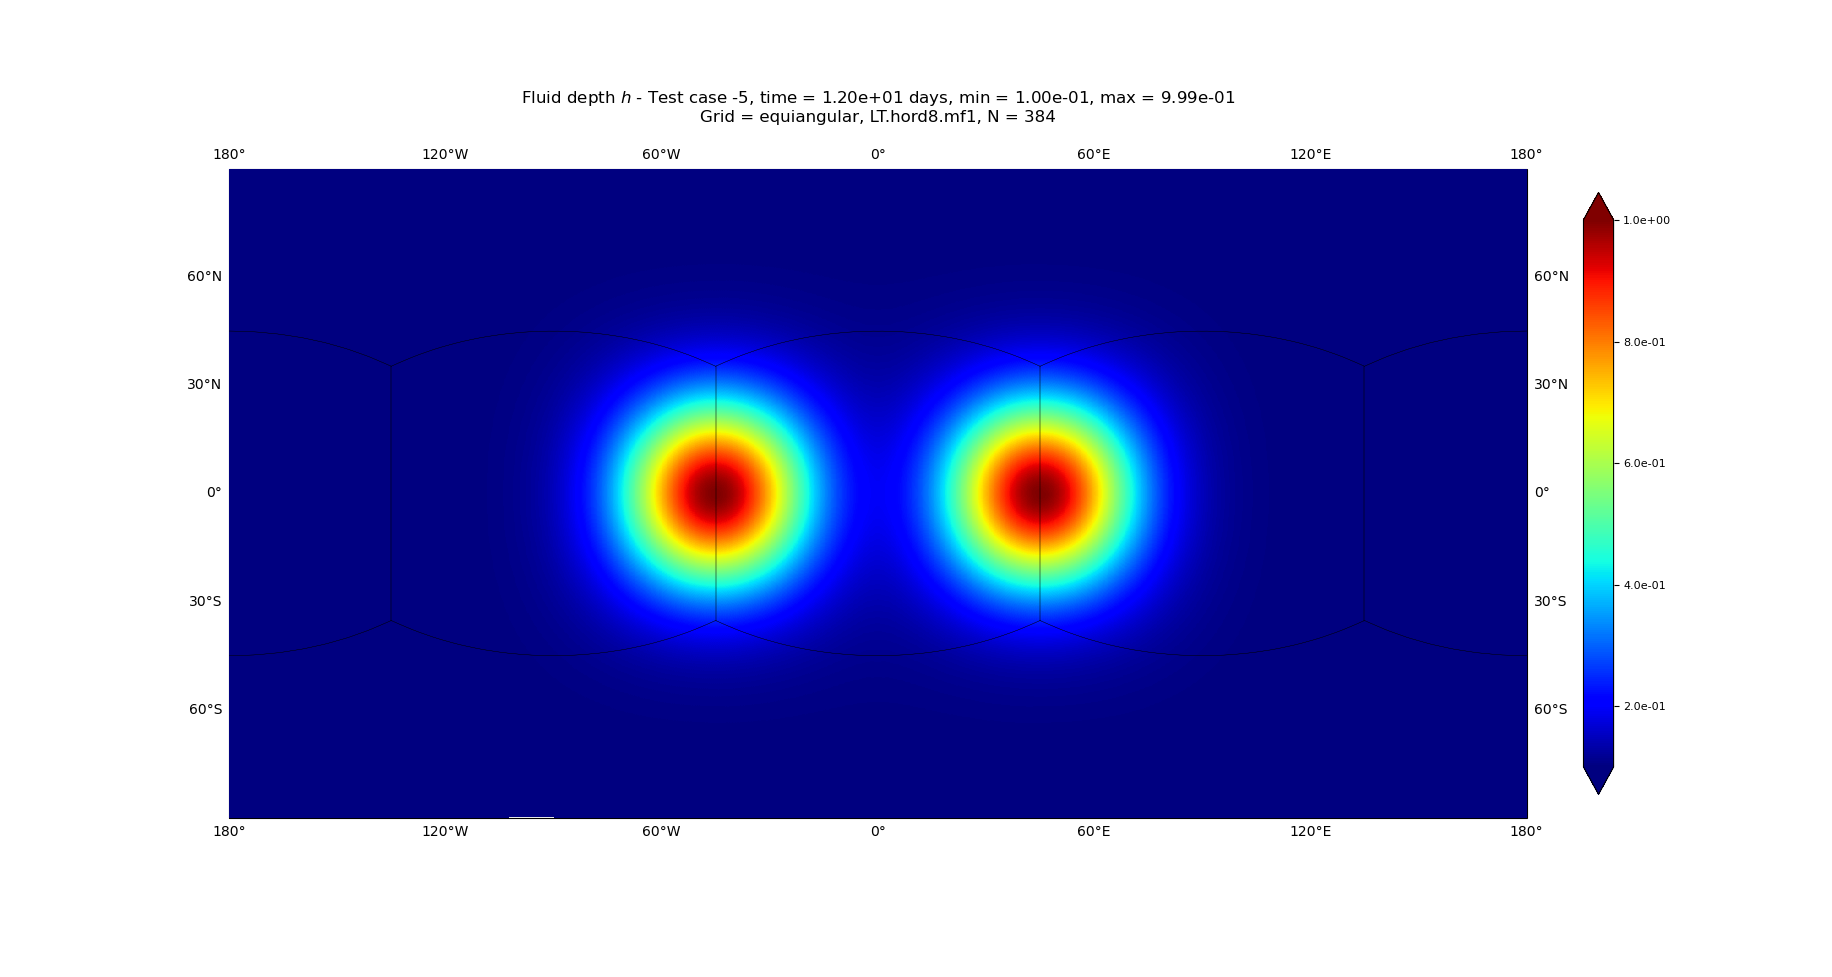
\includegraphics[width=1\linewidth]{h_tc-5_t12_alpha0_C384_g2_dg2_adv2_hord8_mf1_tf12}
		\caption{$t=12$ days.\label{chp-advcs-sec-exp-adv3-f}}
	\end{subfigure}
	\caption{Similar to Figure \ref{chp-advcs-sec-exp-adv2} but using IC2 and VF2 from Table \ref{chp5-ic}.\label{chp-advcs-sec-exp-adv3}}
\end{figure}

\newpage
\begin{figure}[!htb]
	\centering
	\begin{subfigure}{0.45\textwidth}
		\centering
		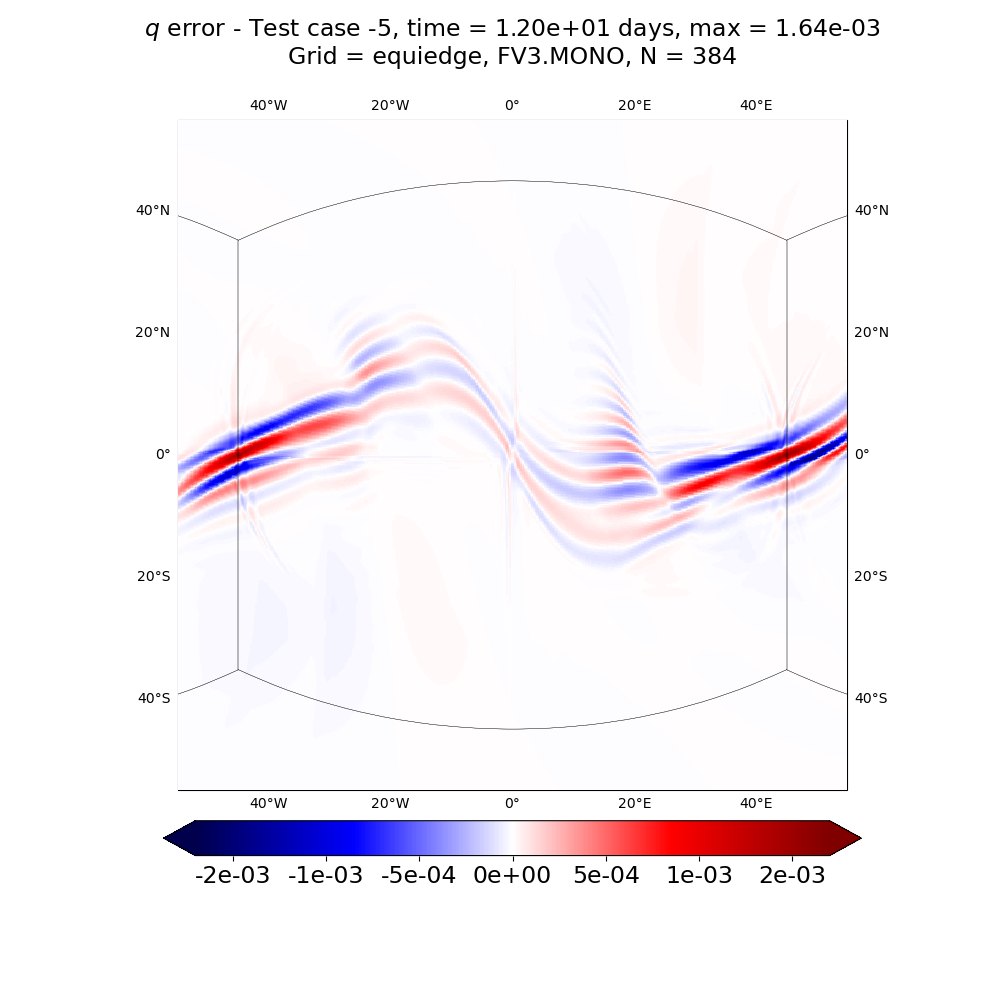
\includegraphics[width=1\linewidth]{h_error_tc-5_t12_alpha0_C384_g0_dg2_adv1_hord8_mf1_tf12}
		\caption{PL scheme.\label{chp-advcs-sec-exp-adv3-errors-0a}}
	\end{subfigure}
	\begin{subfigure}{0.45\textwidth}
		\centering
		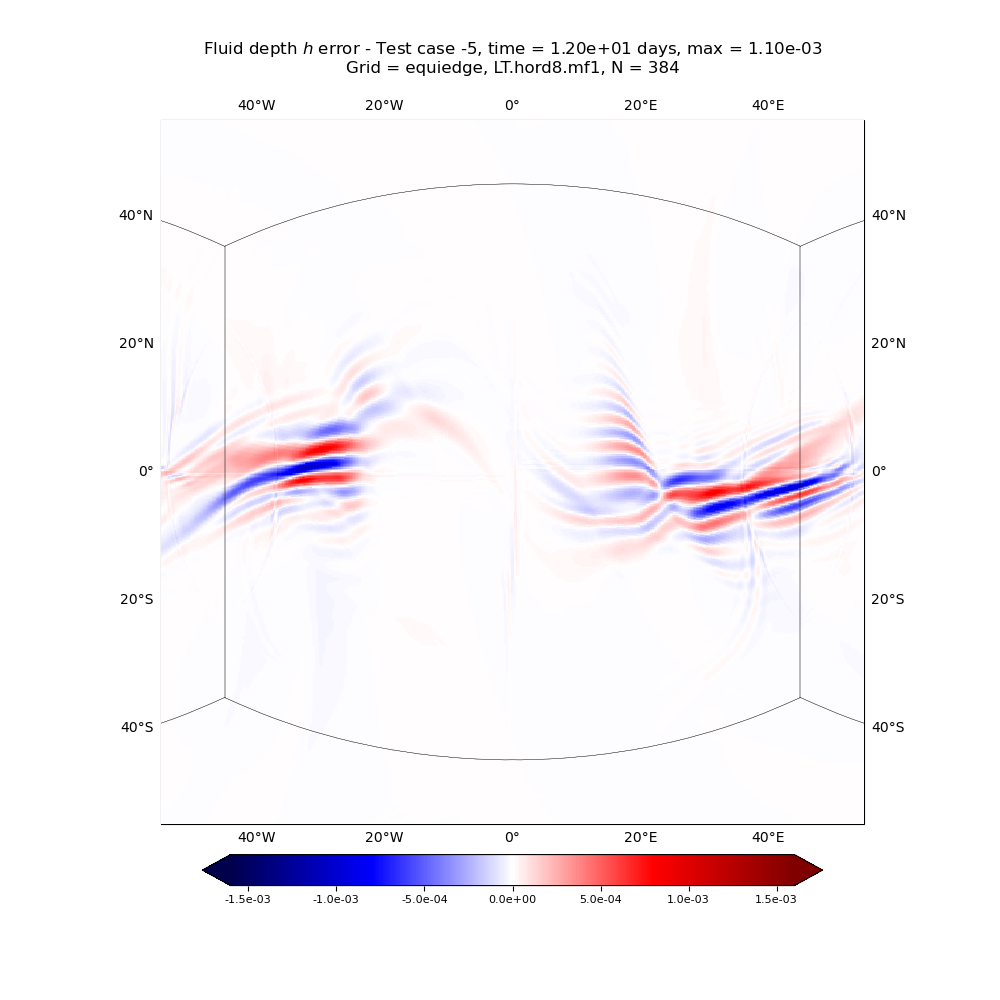
\includegraphics[width=1\linewidth]{h_error_tc-5_t12_alpha0_C384_g0_dg2_adv2_hord8_mf1_tf12}
		\caption{LT scheme.\label{chp-advcs-sec-exp-adv3-errors-0b}}
	\end{subfigure}
	\caption{
		Advection experiment errors using IC2 and VF2 from Table \ref{chp5-ic} after 12 days, using hord8
		with PL (left) and LT schemes (right) on the g0 grid with $N=384$. 
		 \label{chp-advcs-sec-exp-adv3-errors-0}}
\end{figure}
\begin{figure}[!htb]
	\centering
	\begin{subfigure}{0.45\textwidth}
		\centering
		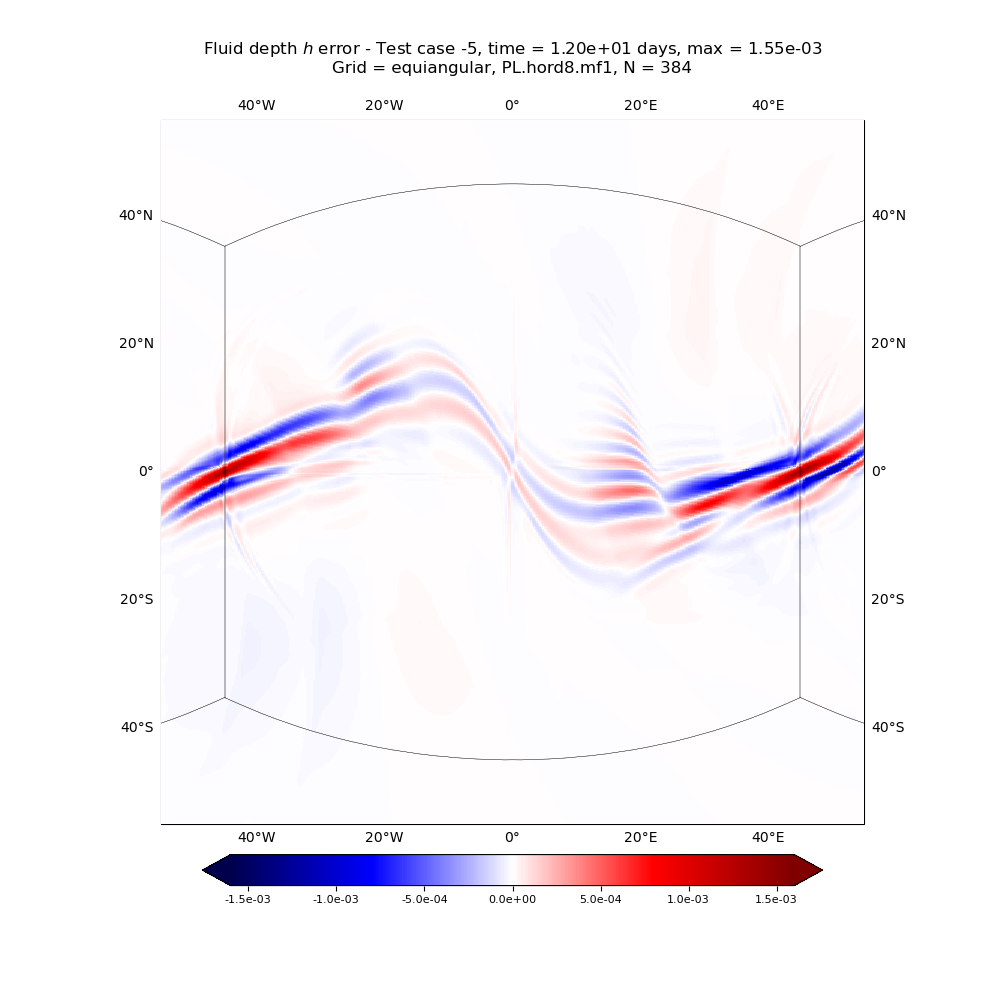
\includegraphics[width=1\linewidth]{h_error_tc-5_t12_alpha0_C384_g2_dg2_adv1_hord8_mf1_tf12}
		\caption{PL scheme.\label{chp-advcs-sec-exp-adv3-errors-2a}}
	\end{subfigure}
	\begin{subfigure}{0.45\textwidth}
		\centering
		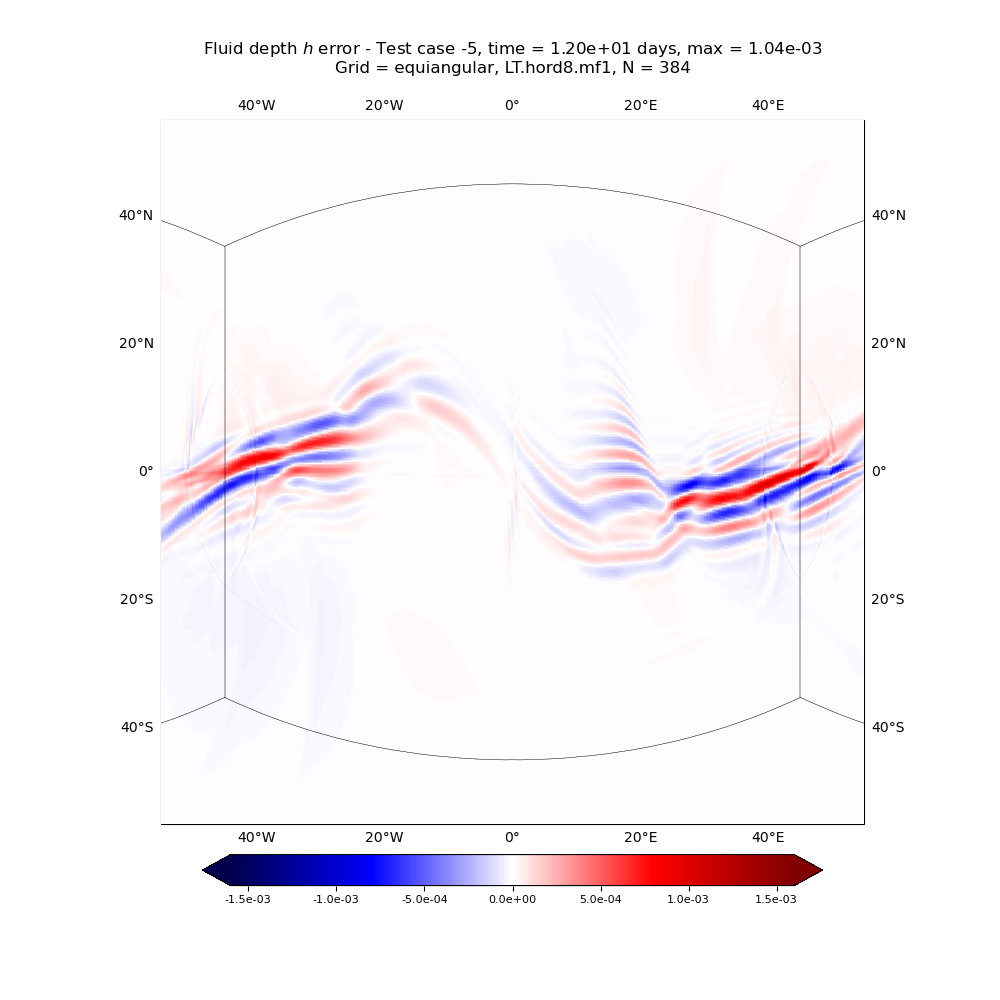
\includegraphics[width=1\linewidth]{h_error_tc-5_t12_alpha0_C384_g2_dg2_adv2_hord8_mf1_tf12}
		\caption{LT scheme.\label{chp-advcs-sec-exp-adv3-errors-2b}}
	\end{subfigure}
	\caption{As Figure \ref{chp-advcs-sec-exp-adv3-errors-0} but using the g2 grid.\label{chp-advcs-sec-exp-adv3-errors-2}}
\end{figure}


\newpage
\begin{figure}[!htb]
	\centering
	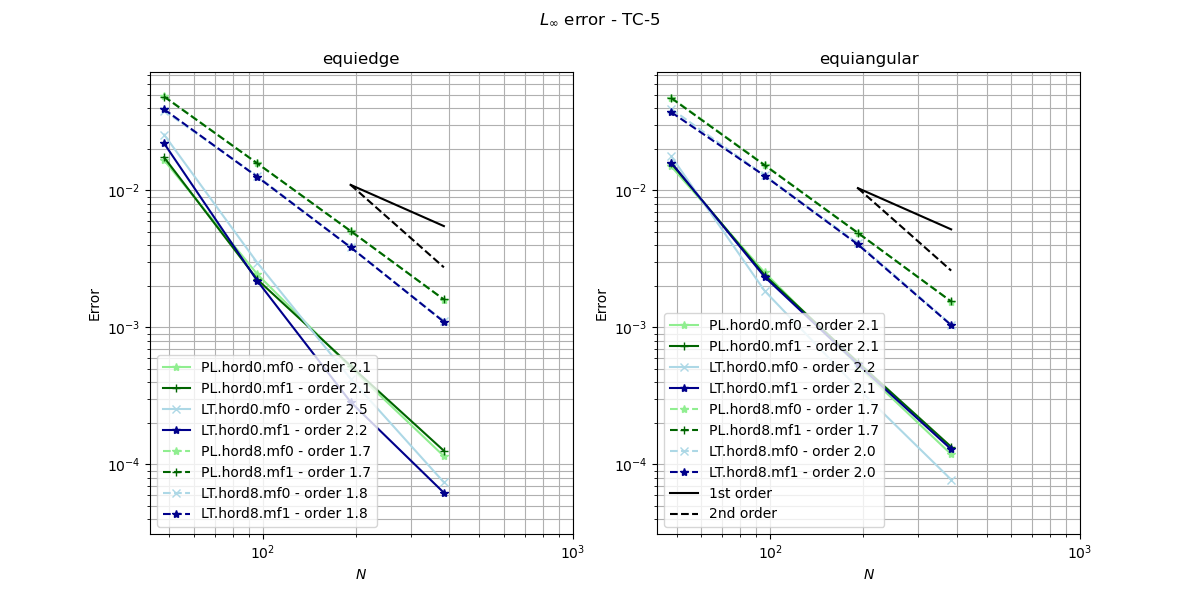
\includegraphics[width=1\linewidth]{linferror_tc-5_alpha0}
	\caption{As Figure \ref{chp-advcs-sec-exp-adv2-linf} but using  IC2 and VF2 from Table \ref{chp5-ic}.\label{chp-advcs-sec-exp-adv3-linf}}
\end{figure}

\begin{figure}[!htb]
	\centering
	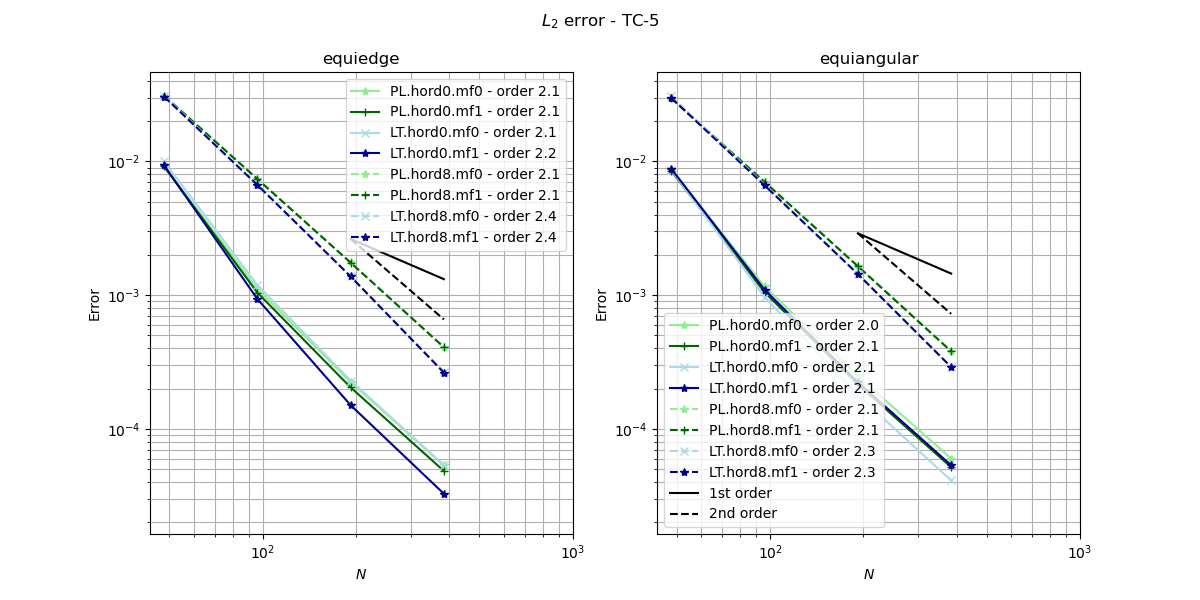
\includegraphics[width=1\linewidth]{l2error_tc-5_alpha0}
	\caption{As Figure \ref{chp-advcs-sec-exp-adv3-linf} but considering the $L_2$ norm. \label{chp-advcs-sec-exp-adv3-error}}
\end{figure}


\newpage
\subsection{Divergent deformational flow}
The fifth and last test case consider the divergent wind VF3 from table \ref{chp5-tab2} along with
the initial condition IC2 from table \ref{chp5-tab1}.
This test is also suggested by \citet{nair:2010} and the their paper shows how the solution evolves over time.
\begin{figure}[!htb]
	\centering
	\begin{subfigure}{0.45\textwidth}
		\centering
		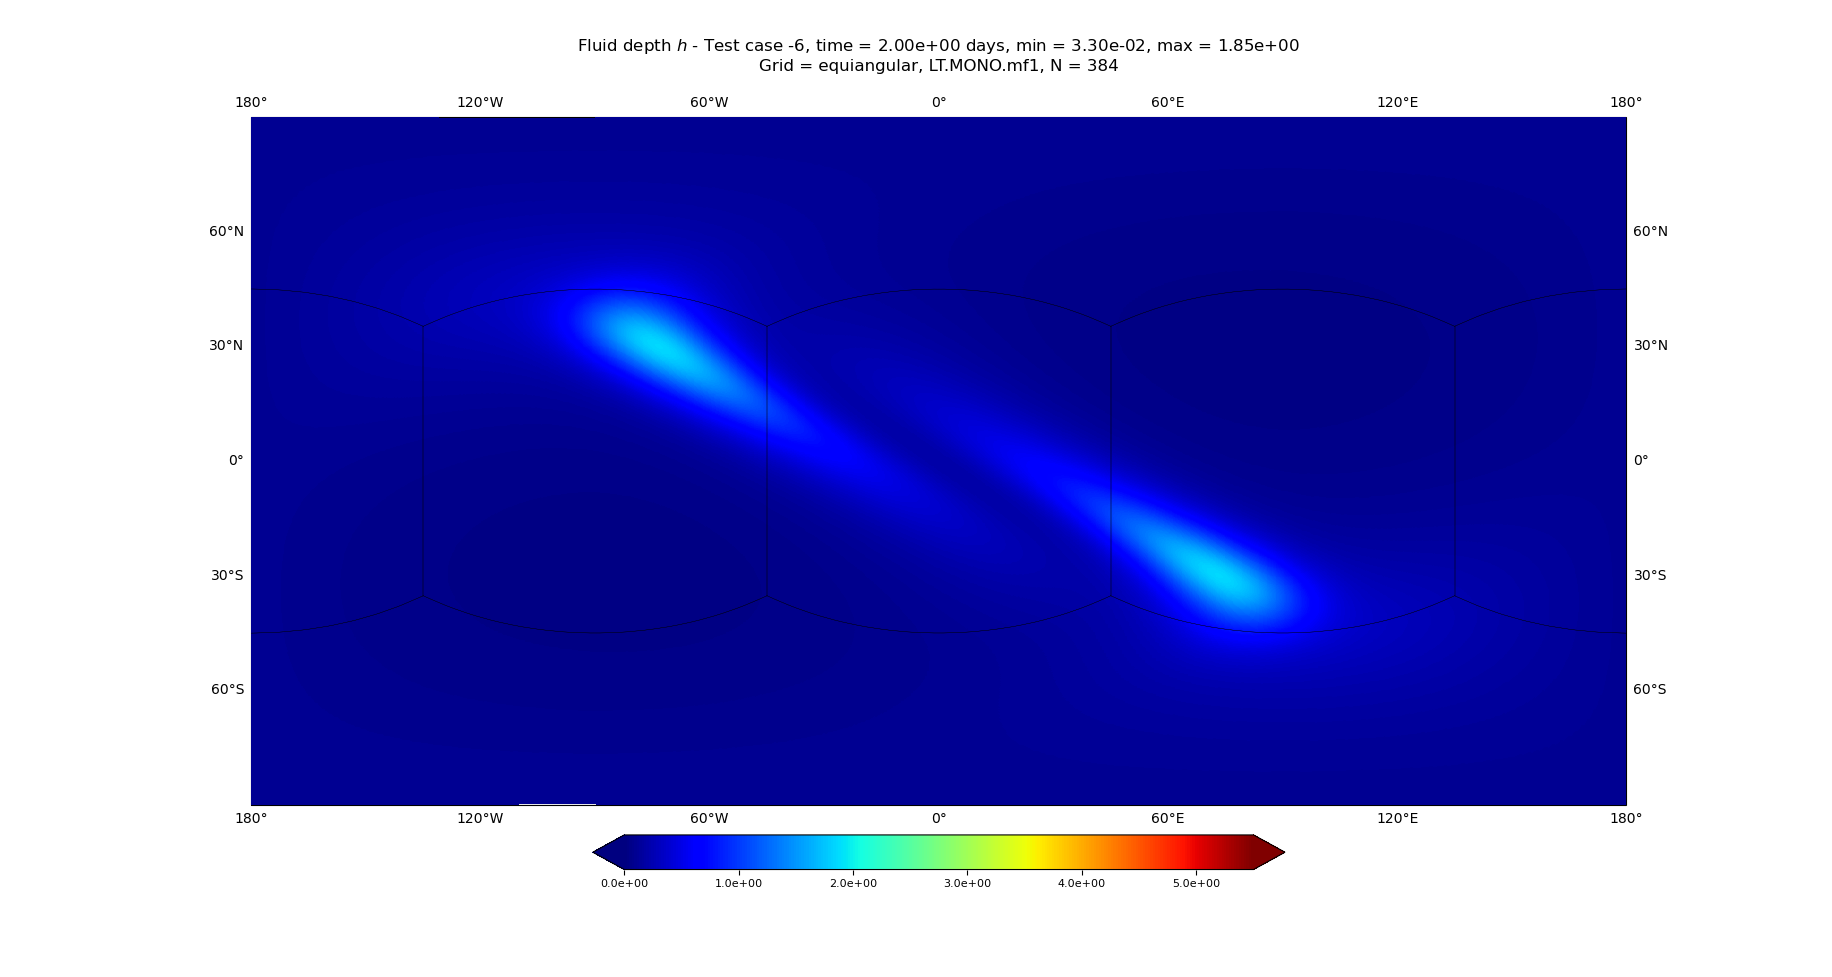
\includegraphics[width=1\linewidth]{h_tc-6_t2_alpha0_C384_g2_dg2_adv2_hord8_mf1_tf12}
		\caption{$t=2$ days.\label{chp-advcs-sec-exp-adv4-a}}
	\end{subfigure}
	\begin{subfigure}{0.45\textwidth}
		\centering
		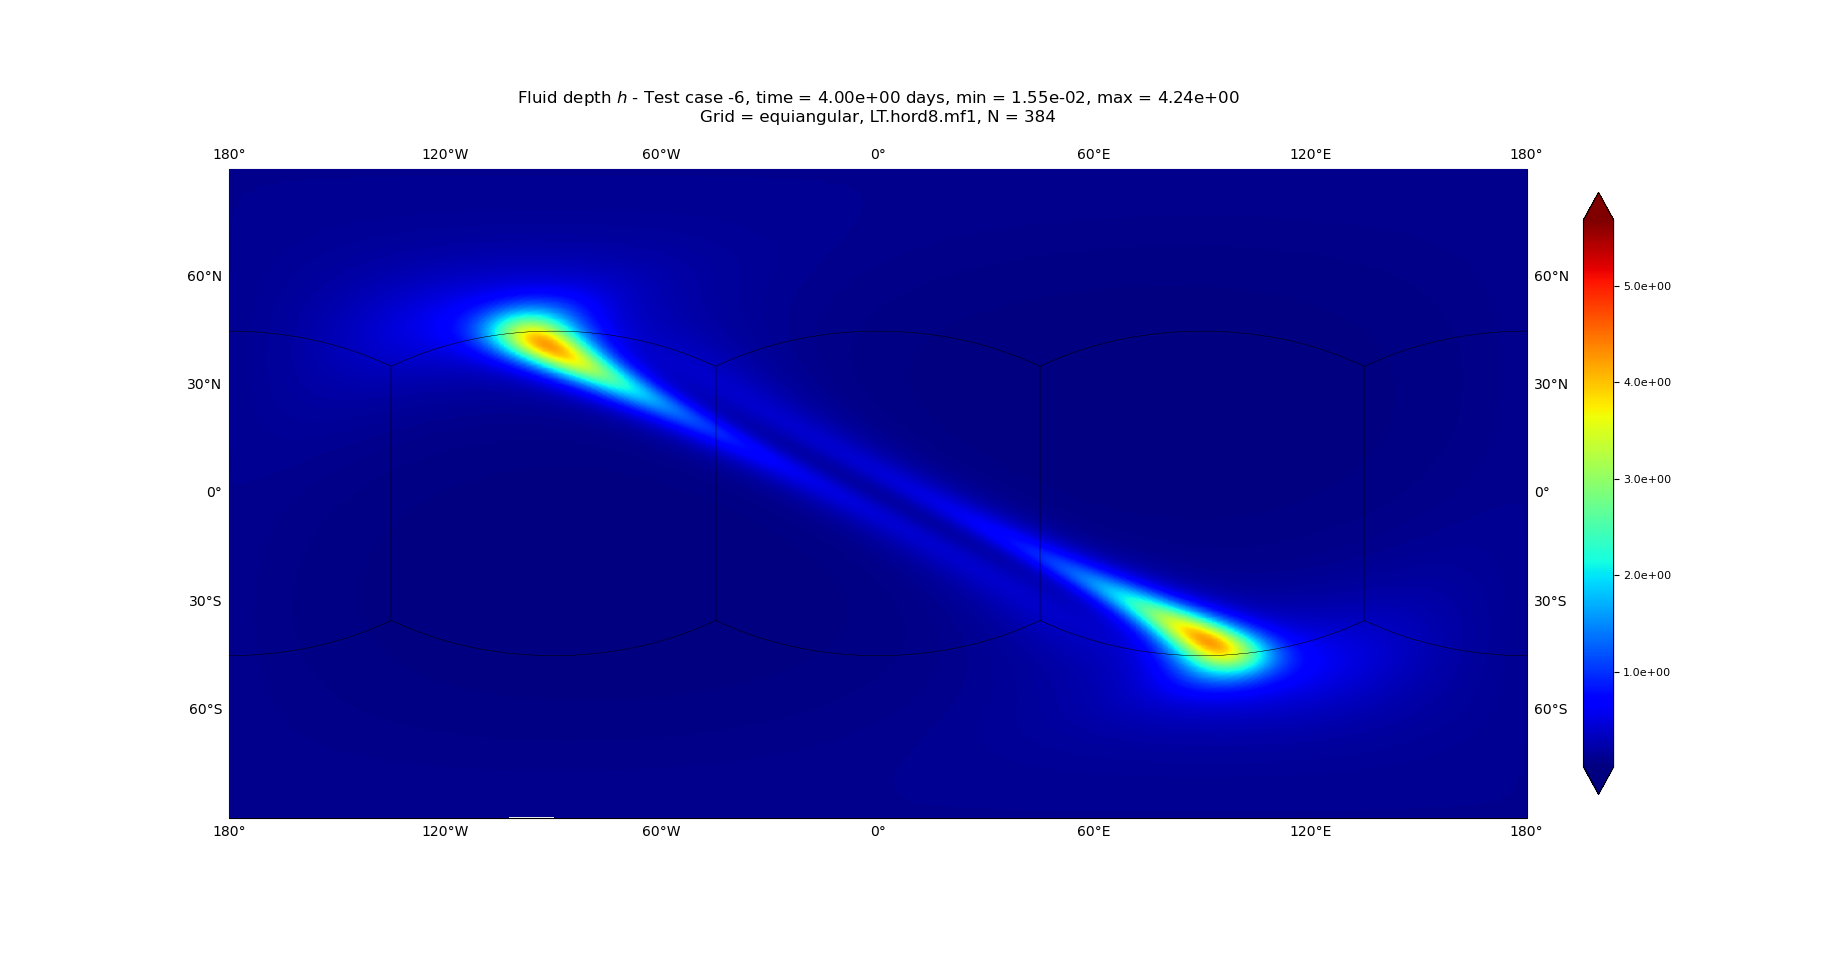
\includegraphics[width=1\linewidth]{h_tc-6_t4_alpha0_C384_g2_dg2_adv2_hord8_mf1_tf12}
		\caption{$t=4$ days.\label{chp-advcs-sec-exp-adv4-b}}
	\end{subfigure}

	\begin{subfigure}{0.45\textwidth}
		\centering
		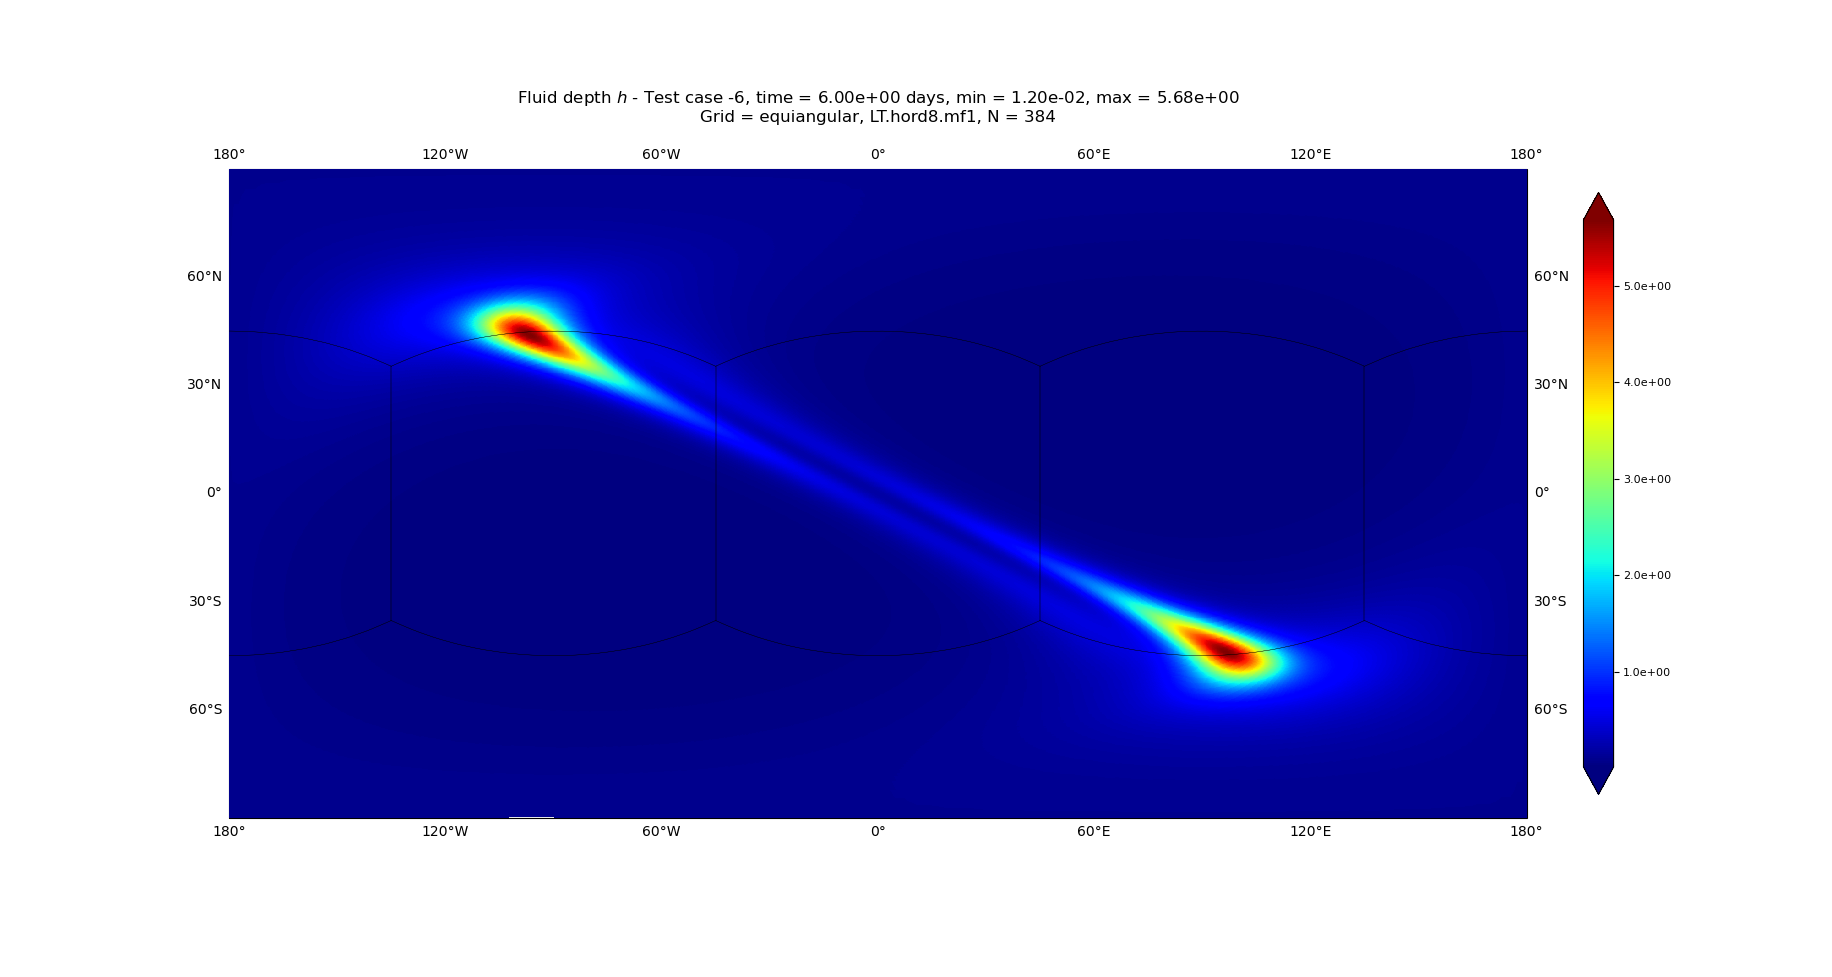
\includegraphics[width=1\linewidth]{h_tc-6_t6_alpha0_C384_g2_dg2_adv2_hord8_mf1_tf12}
		\caption{$t=6$ days.\label{chp-advcs-sec-exp-adv4-c}}
	\end{subfigure}
	\begin{subfigure}{0.45\textwidth}
		\centering
		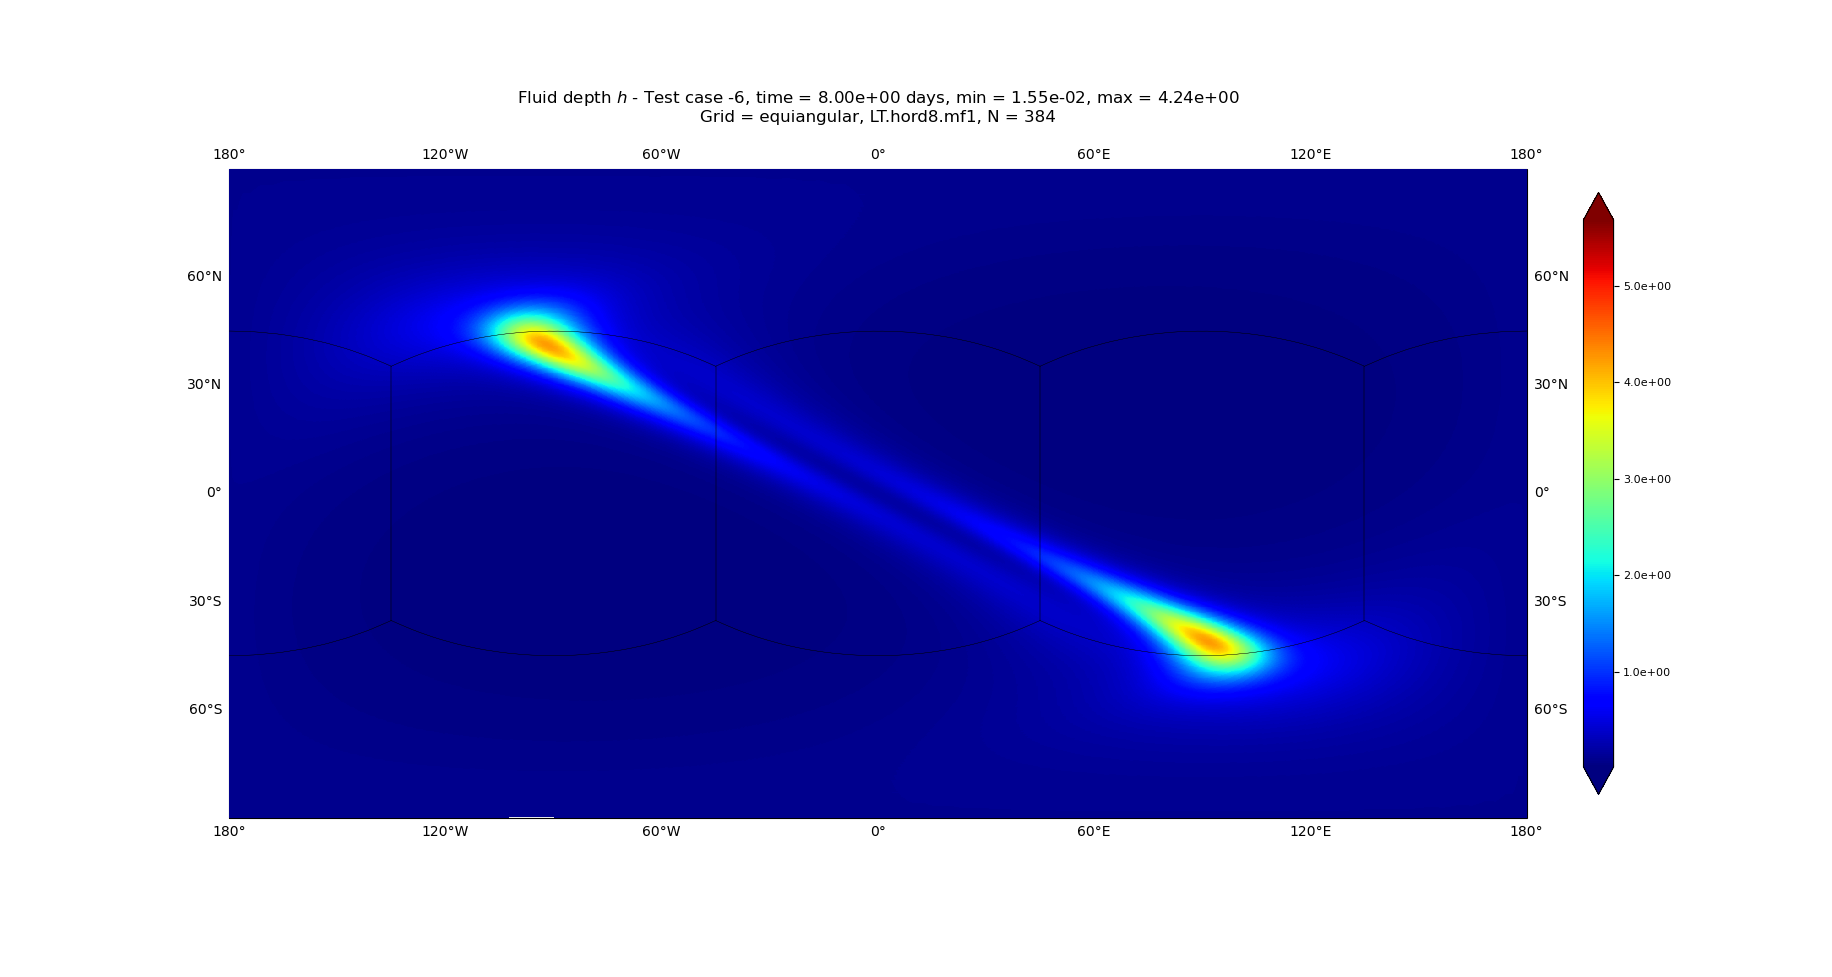
\includegraphics[width=1\linewidth]{h_tc-6_t8_alpha0_C384_g2_dg2_adv2_hord8_mf1_tf12}
		\caption{$t=8$ days.\label{chp-advcs-sec-exp-adv4-d}}
	\end{subfigure}

	\begin{subfigure}{0.45\textwidth}
		\centering
		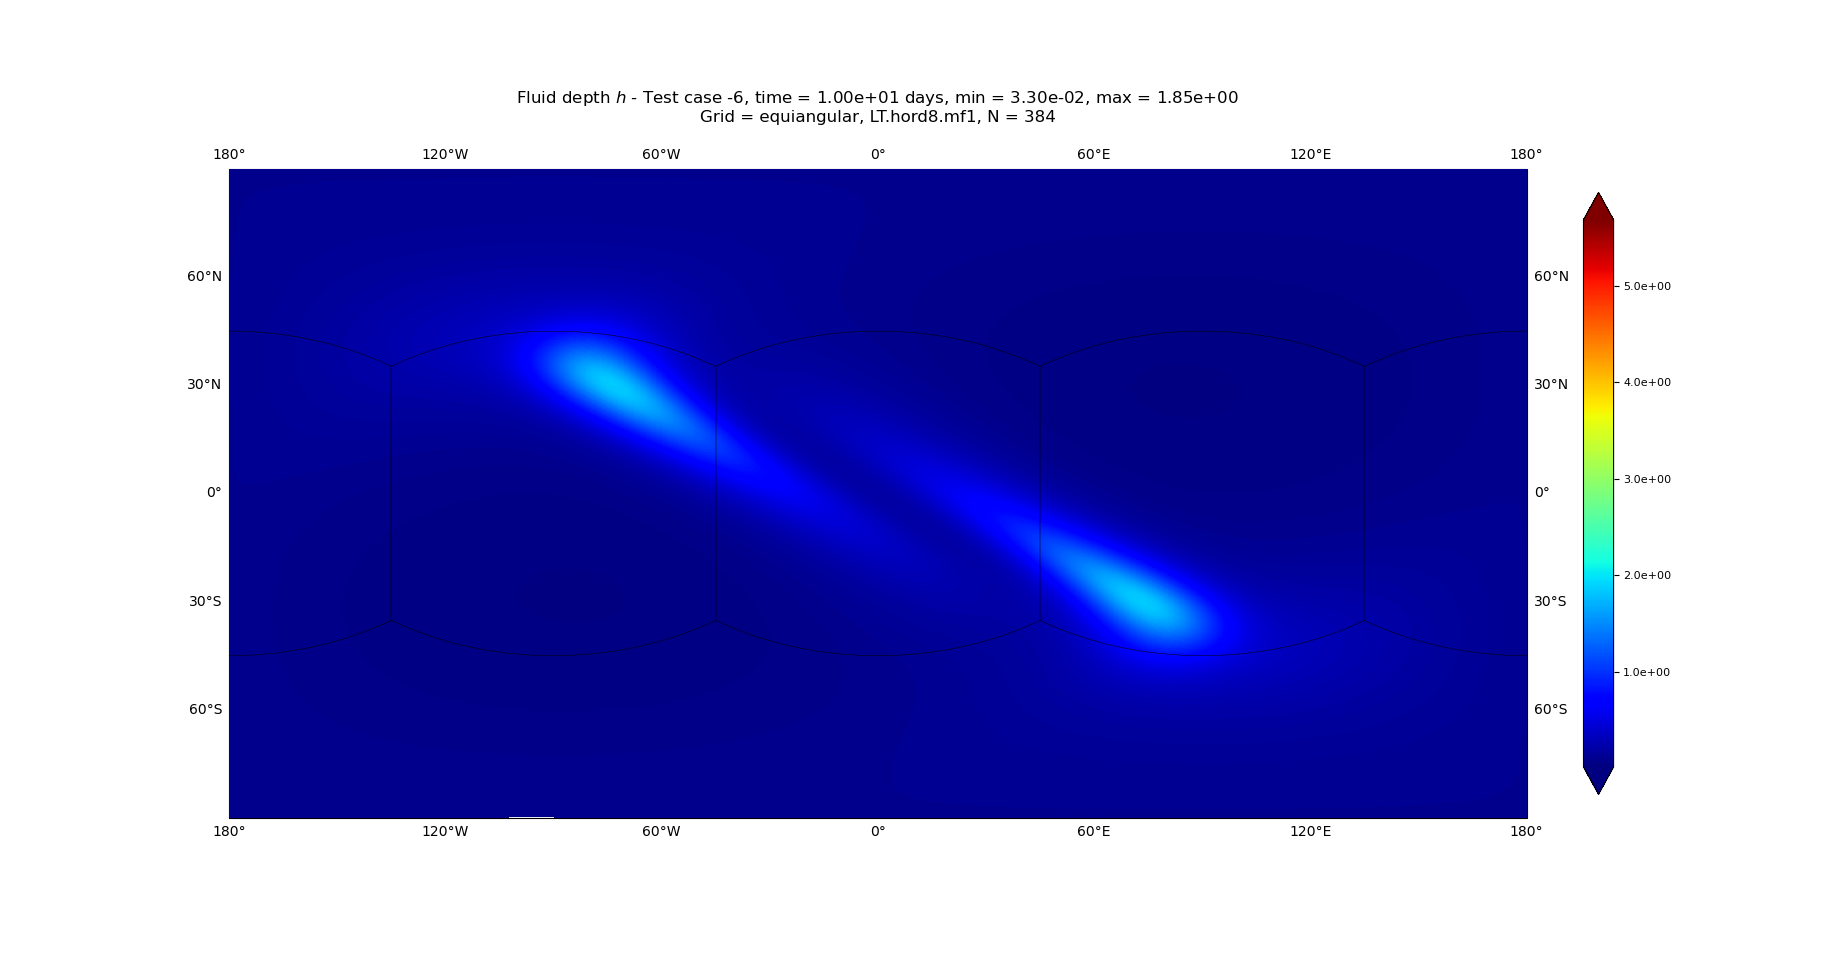
\includegraphics[width=1\linewidth]{h_tc-6_t10_alpha0_C384_g2_dg2_adv2_hord8_mf1_tf12}
		\caption{$t=10$ days.\label{chp-advcs-sec-exp-adv4-e}}
	\end{subfigure}
	\begin{subfigure}{0.45\textwidth}
		\centering
		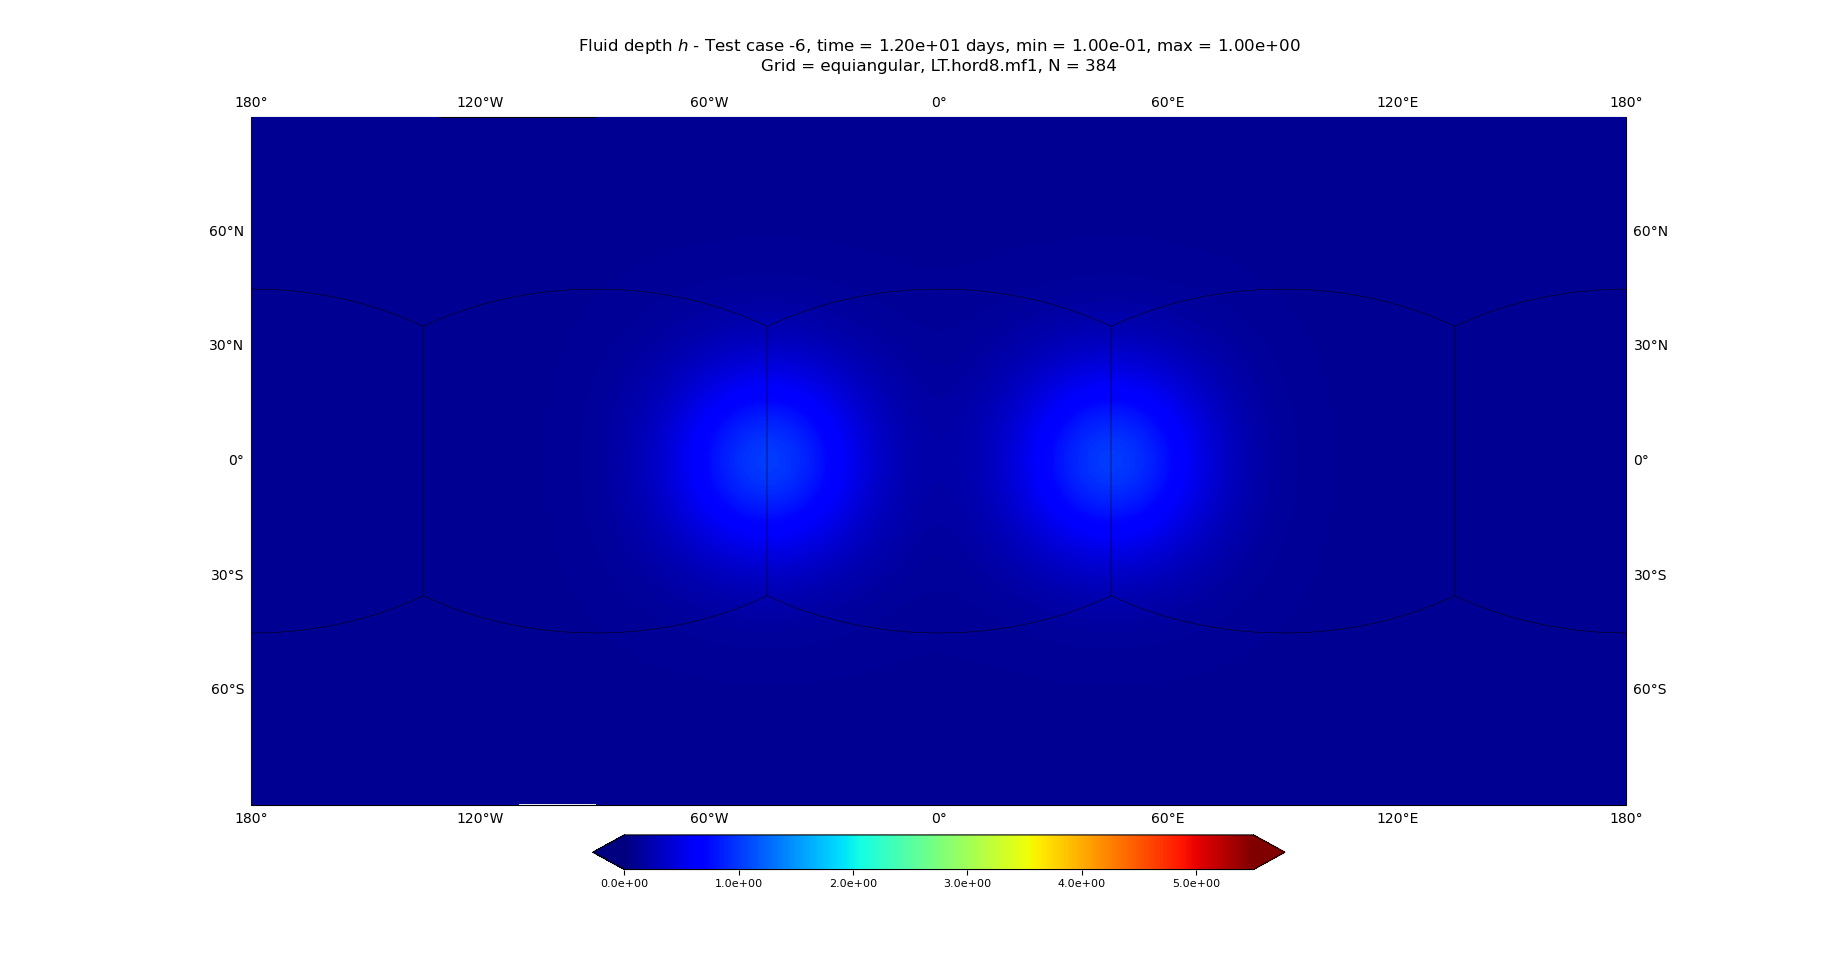
\includegraphics[width=1\linewidth]{h_tc-6_t12_alpha0_C384_g2_dg2_adv2_hord8_mf1_tf12}
		\caption{$t=12$ days.\label{chp-advcs-sec-exp-adv4-f}}
	\end{subfigure}
	\caption{Similar to Figure \ref{chp-advcs-sec-exp-adv2} but using IC2 and VF3 from Table \ref{chp5-ic}.\label{chp-advcs-sec-exp-adv4}}
\end{figure}

\newpage
\begin{figure}[!htb]
	\centering
	\begin{subfigure}{0.45\textwidth}
		\centering
		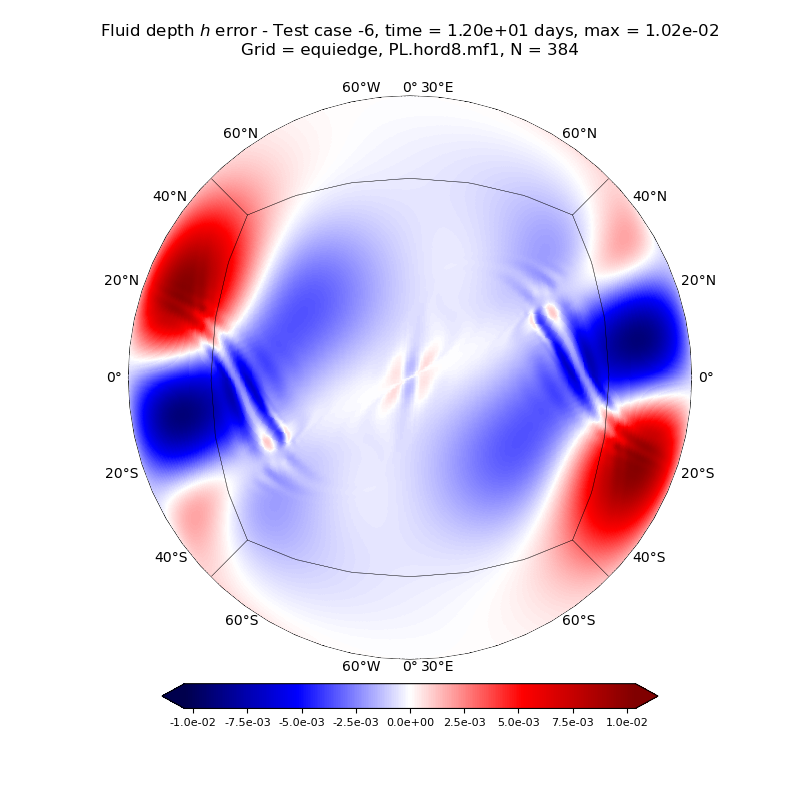
\includegraphics[width=1\linewidth]{h_error_tc-6_t12_alpha0_C384_g0_dg2_adv1_hord8_mf1_tf12}
		\caption{PL scheme.\label{chp-advcs-sec-exp-adv4-errors-0a}}
	\end{subfigure}
	\begin{subfigure}{0.45\textwidth}
		\centering
		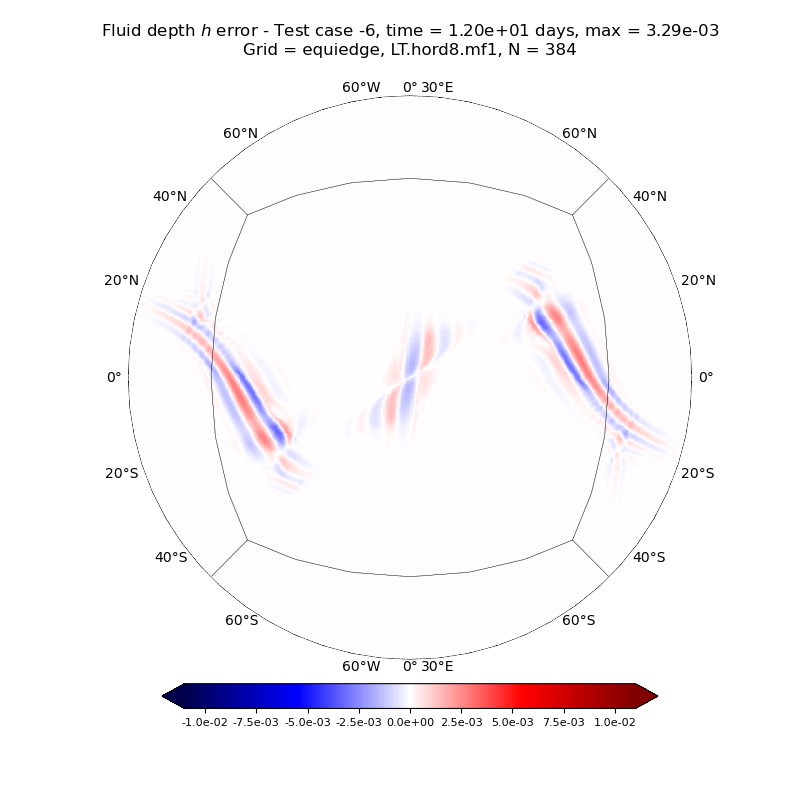
\includegraphics[width=1\linewidth]{h_error_tc-6_t12_alpha0_C384_g0_dg2_adv2_hord8_mf1_tf12}
		\caption{LT scheme.\label{chp-advcs-sec-exp-adv4-errors-0b}}
	\end{subfigure}
	\caption{
	 Advection experiment errors using IC2 and VF3 from Table \ref{chp5-ic} after 12 days, using hord8
	 with PL (left) and LT schemes (right) on the g0 grid with $N=384$.
	 \label{chp-advcs-sec-exp-adv4-errors-0}}
\end{figure}
\begin{figure}[!htb]
	\centering
	\begin{subfigure}{0.45\textwidth}
		\centering
		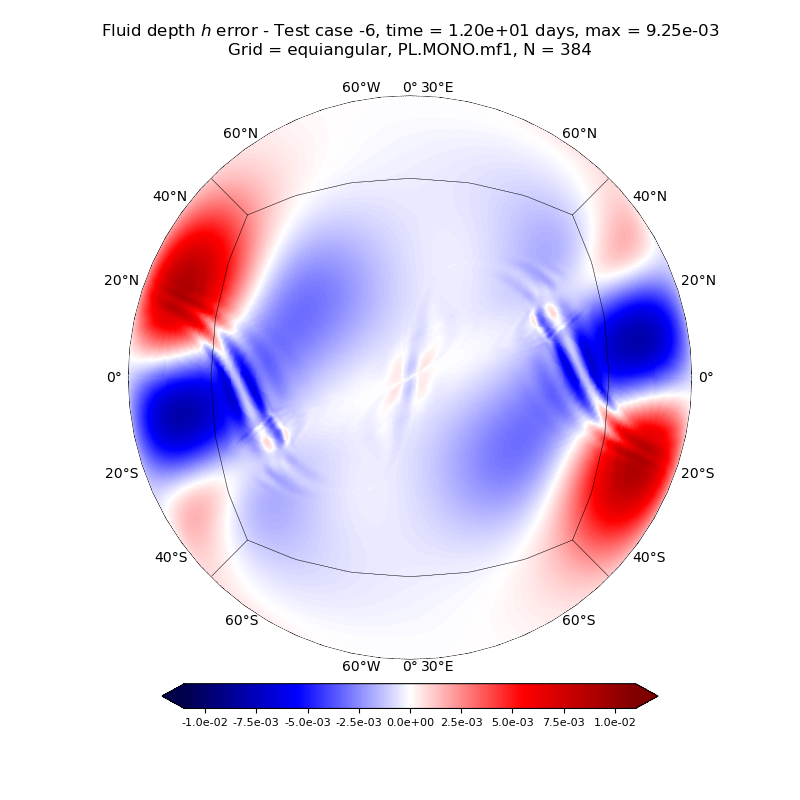
\includegraphics[width=1\linewidth]{h_error_tc-6_t12_alpha0_C384_g2_dg2_adv1_hord8_mf1_tf12}
		\caption{PL scheme.\label{chp-advcs-sec-exp-adv4-errors-2a}}
	\end{subfigure}
	\begin{subfigure}{0.45\textwidth}
		\centering
		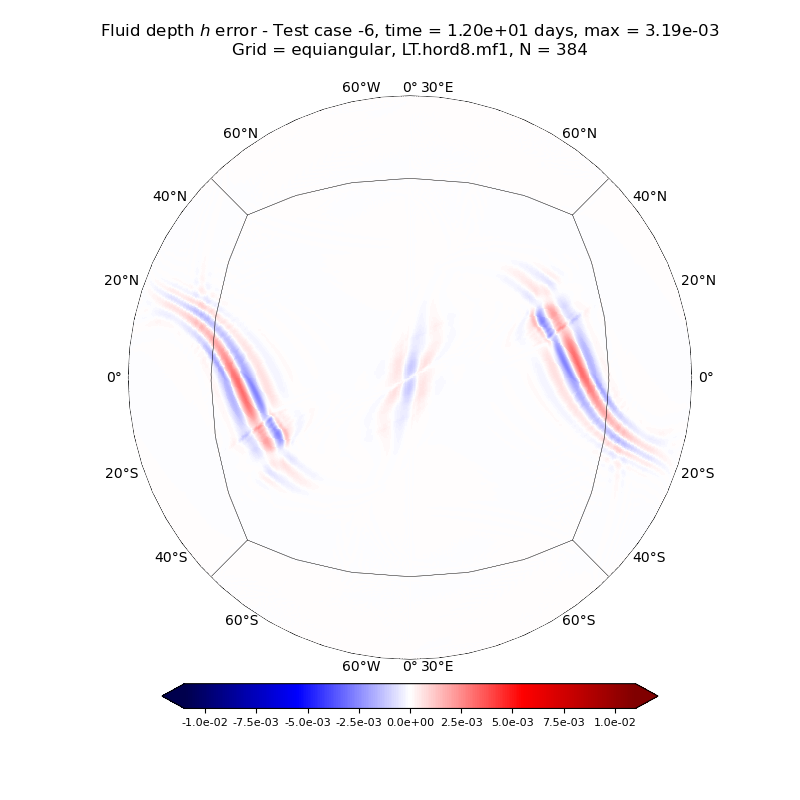
\includegraphics[width=1\linewidth]{h_error_tc-6_t12_alpha0_C384_g2_dg2_adv2_hord8_mf1_tf12}
		\caption{LT scheme.\label{chp-advcs-sec-exp-adv4-errors-2b}}
	\end{subfigure}
	\caption{As Figure \ref{chp-advcs-sec-exp-adv4-errors-0} but using the g2 grid.\label{chp-advcs-sec-exp-adv4-errors-2}}
\end{figure}



\newpage

\begin{figure}[!htb]
	\centering
	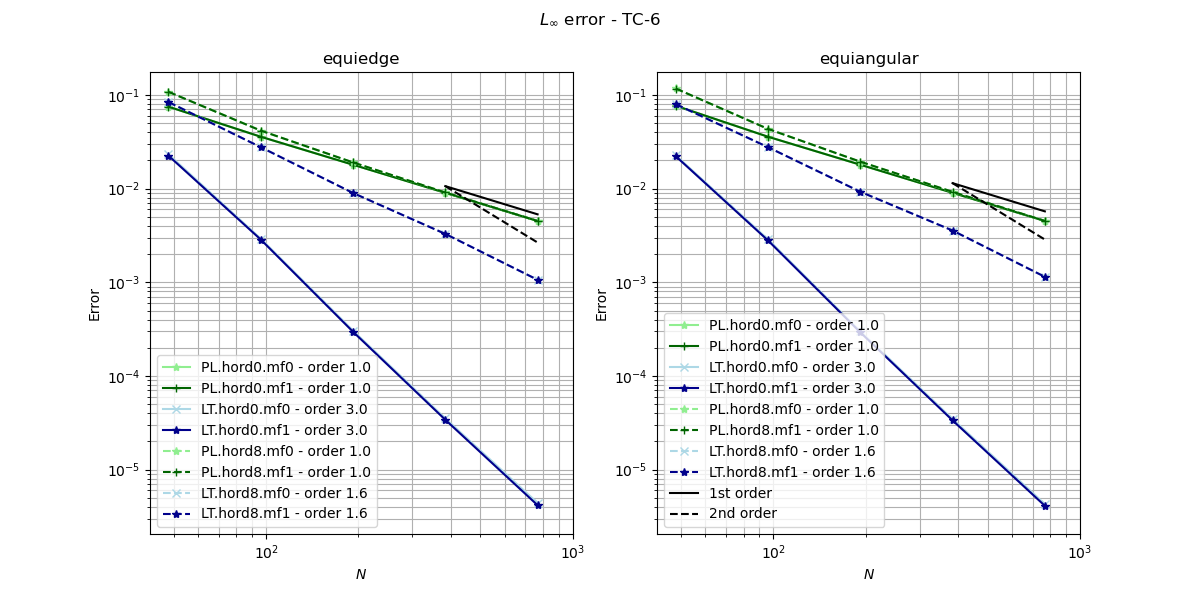
\includegraphics[width=1\linewidth]{linferror_tc-6_alpha0}
	\caption{As Figure \ref{chp-advcs-sec-exp-adv2-linf} but using  IC2 and VF3 from Table \ref{chp5-ic}.\label{chp-advcs-sec-exp-adv4-linf}}
\end{figure}

\begin{figure}[!htb]
	\centering
	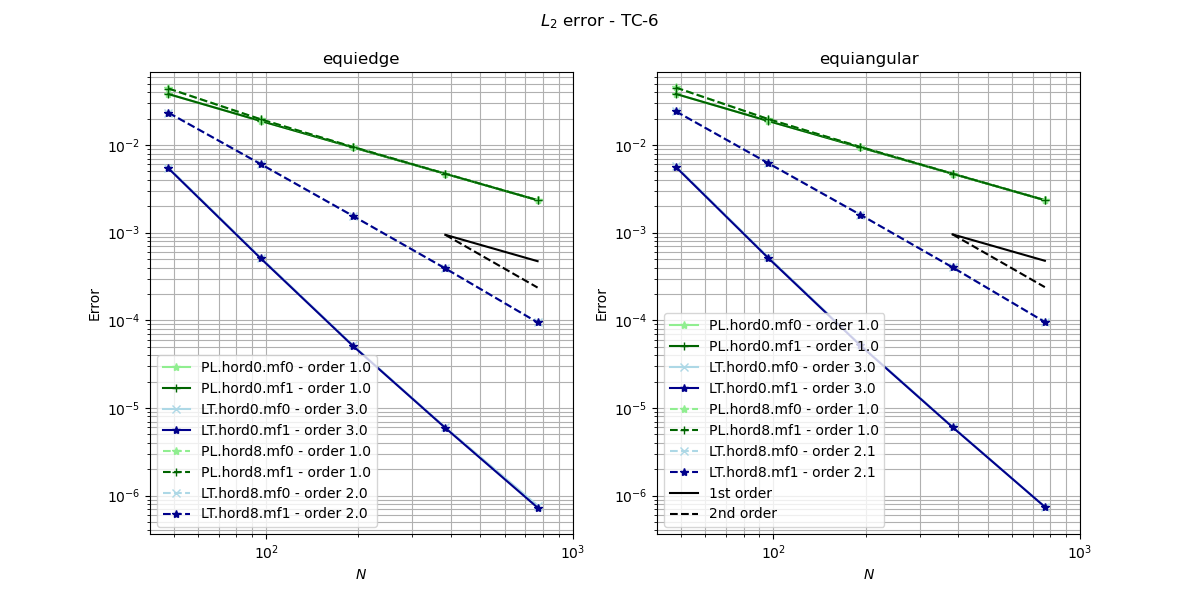
\includegraphics[width=1\linewidth]{l2error_tc-6_alpha0}
	\caption{As Figure \ref{chp-advcs-sec-exp-adv4-linf} but considering the $L_2$ norm. \label{chp-advcs-sec-exp-adv4-error}}
\end{figure}

\newpage
\section{Concluding remarks}
\label{chp-cs-conc}